\documentclass[10pt]{article}
\usepackage[margin=1in]{geometry}
\usepackage{booktabs,graphicx,hyperref}
\usepackage[T1]{fontenc}
\usepackage[utf8]{inputenc}
\title{How Much Can Be Added on Top of Existing KV-Cache and Weight Formats? An Empirical Study of Lossless and Lossy Compression for GPU-Resident LLM Inference on a Consumer GPU}
\author{NeoXider}
\date{v3.0, 2026-10-23}
\begin{document}
\maketitle

NeoXider --- v3.0, 2026-10-23

This is an empirical measurement study and most of what it reports is negative. We do not propose a new
method. Every number was measured, apart from the rows marked * (analytic projection, still to be validated
on that hardware). Table IDs R1--R87 point to \texttt{RESULTS.md} in the companion repository. An independent
novelty review checked the references marked [abs] / [full*] / [gh] against the abstract, the full text
(HTML extraction) or the GitHub issue/PR; whatever was left unchecked carries [verify].

\begin{abstract}
On one RTX 3090 (24 GB) running llama.cpp we measured how much compression can be stacked \emph{on top of}
the KV-cache formats already in use (F16, Q8\_0, Q4\_0) and the weight formats already in use (BF16, Q8\_0,
Q4\_K\_M), and what that does to memory, speed and answer quality. (i) For IEEE F16 KV of Qwen3-4B, field
entropy shows that only the exponent is compressible: about 2.9--3.3 of 5 bits order-0, and 2.4--2.5 bits
once we condition on channel and previous token. The 10-bit mantissa does not compress. Our context-aware
estimate gives 13.2--13.4 bits per value (--16\ldots{}17\%), and a TRACE-style channel-major bit-plane + zstd codec
reaches 0.835--0.863. Neither figure moves much across code, English and Russian text, nor between 4K and
30K tokens. On BF16 KV of the same model the same codec reaches 0.65--0.68 (1.48--1.53$\times$), because BF16
carries 3 fewer noise mantissa bits. So the dtype, not the codec, accounts for most of the distance to
TRACE's 1.81--1.88$\times$ on BF16 KV.
(ii) A fixed-rate, GPU-addressable exponent format of the kind ZipServ/SplitZip use saves only 4--7\% on F16
KV; in our non-fused scalar read kernel it is also 1.3--1.5$\times$ slower than reading F16. (iii) Lossless coding
on top of llama.cpp's Q8\_0/Q4\_0 KV blocks saves 7--21\% with variable-rate coders. Every fixed-rate variant
we built ends up larger than its base. (iv) Using an exact write-path emulation and real packed types in
llama.cpp, with both K and V quantized, we measure KL, tasks and needle retrieval for lossy variants on top
of each base. F16 with 4 mantissa bits dropped (12 bits) matches Q8\_0 quality: KL 0.0028 vs F16 KV, against
a 0.0024 noise floor. 4-bit KV that keeps the 2 largest of every 128 values exact halves the KL of
llama.cpp's q4\_0 (0.033 vs 0.068) for 11\% more bytes. Our earlier conclusion that most of the q4\_0 loss
comes from the computation path was an artifact of emulating V only and is withdrawn (R44).
(v) llama.cpp's Q8\_0/Q4\_0 KV cut filled-context process VRAM by 28--60\%, but in this build decode is up to
36--37\% slower at 120K. We tie that to known kernel-path issues. An independent ABBA check shows upstream
PR \#30202 recovers about 70\% of the q8\_0 gap (0.64 $\rightarrow$ 0.86 of F16 at 120K), while PR \#30792 does nothing on
this GPU. (vi) Lossless re-coding of GGUF
k-quant weights has only 2--7\% order-0 headroom. Per-tensor int4 shows 0.8 bits of code entropy, but
group-128 int4 on the same weights shows 3.6 bits, which is how the reported "int4" figures reconcile.
What is actually usable: capacity (fewer KV bytes, longer context) and speed only where a fast kernel exists
(mixed-precision weight recipes: --23\% size and +16--18\% decode at unchanged quality).
(vii) We then implemented the formats as real ggml types with CUDA kernels in a llama.cpp fork and measured
every row with one binary (R80--R87). A lossless fixed-rate BF16 weight type gives bit-identical logits at
0.76 of the tensor size with 1.03--1.05$\times$ decode. A decode kernel that reads each K/V row once per GQA group
makes Q8\_0 / Q4\_0 KV of Qwen3-4B decode 1.11 / 1.16$\times$ as fast as F16 KV at 120K (0.64 / 0.60$\times$ with the stock
kernel) using 38 / 60\% less process memory. A 12-bit KV type saves 20\% of memory at 1.15$\times$ decode. Our
lossless KV type is 1.2--7$\times$ slower and stops being exact once its overflow pool fills. On a hybrid model with
KV in 6 of 24 layers (Qwen3.5-2B) the KV-side changes save at most a few hundred MiB, and the same kernel
loses to the stock path.
\end{abstract}
\section{Introduction}

\subsection{Analytic motivation}

At batch 1, one decode step reads all the weights and the entire KV cache once. When kernels are memory-bound
and decode is fused and cheap, step time follows bytes and capacity follows 1/r. The model in Appendix A
(* projections, calibrated on our 3090 numbers) predicts small speed gains from KV compression at short
context, more of them as context and batch grow, and first-order capacity gains on servers. The rest of the
paper checks which parts of that survive contact with real formats and real kernels.

\subsection{Practical value}

Two benefits are on the table: (1) faster inference, and (2) a longer context or a larger model in the same
VRAM. Measured against projected (*):

\begin{table}[h]\centering\scriptsize
\resizebox{\linewidth}{!}{%
\begin{tabular}{lll}
\toprule
Benefit & Measured on RTX 3090 / llama.cpp & Projected (*) \\
\midrule
Longer context in the same VRAM & Qwen3-4B at a filled 120K context: F16 KV 19,980 MiB $\rightarrow$ Q8\_0 12,352 (--38\%) $\rightarrow$ Q4\_0 8,032 (--60\%) process VRAM (R30). With lazy allocation, process memory follows the filled tokens (144 MiB at 1K vs 4,608 MiB eager at -c 32768, R23; a known technique: vAttention, kvcached, llama.cpp PR \#21757). Our lossy variants on top of F16 (drop 4 bits) reach Q8\_0-like quality at 12 of 16 bits (R36) & Lossless F16 KV --16\% would add about 1.2$\times$ context; a model that "almost fits" (32B Q5\_K\_M, 22.8 GB) fits after $\times$0.934 (*) \\
Faster decode & Mixed-precision weight recipes inside llama.cpp: BF16 + FFN$\rightarrow$Q8\_0 is --23\% size and +16--18\% decode at unchanged KL and tasks (R34, speed R37, Qwen3.5-2B; a known practice: \texttt{llama-quantize --tensor-type}, PR \#12511). Quantized KV in this llama.cpp build is \emph{slower} (R25); upstream PR \#30202 recovers about 70\% of the Q8\_0 gap (R39). Our lossless KV formats are slower in a non-fused kernel (R22, R26) & Up to about 3$\times$ at long context with Q4-class KV \emph{if} kernels stay bandwidth-bound (Appendix A *); depends entirely on kernel quality \\
\bottomrule
\end{tabular}}
\end{table}

Who gains what (status: M = measured on our machine, P* = projection):

\begin{table}[h]\centering\scriptsize
\resizebox{\linewidth}{!}{%
\begin{tabular}{llll}
\toprule
Setting & Speed gain & Capacity gain & Status \\
\midrule
Consumer GPU with little VRAM, short context & weights: +2--18\% from mixed-precision recipes & weights --10\ldots{}23\% & M \\
Consumer GPU, long context (32K--120K) & none in llama.cpp today (quantized KV 27--37\% slower; 8--14\% slower for Q8\_0 with PR \#30202, R39) & KV --28\ldots{}--60\% (Q8\_0/Q4\_0); lossless F16 $\approx$ --16\% (CPU codec) & M \\
PCIe offload of layers & $\approx$ 1/r on the streamed part if decode is on GPU & --- & P* \\
Server GPU with large batch & bandwidth-bound regime makes KV bytes matter more; scalar llama.cpp-style decoders are projected to lose (Appendix A; FP8 tensor-core kernels of server stacks are not modelled) & batch $\times$ context capacity $\approx$ 1/r & P* \\
\bottomrule
\end{tabular}}
\end{table}


\begin{figure}[htbp]\centering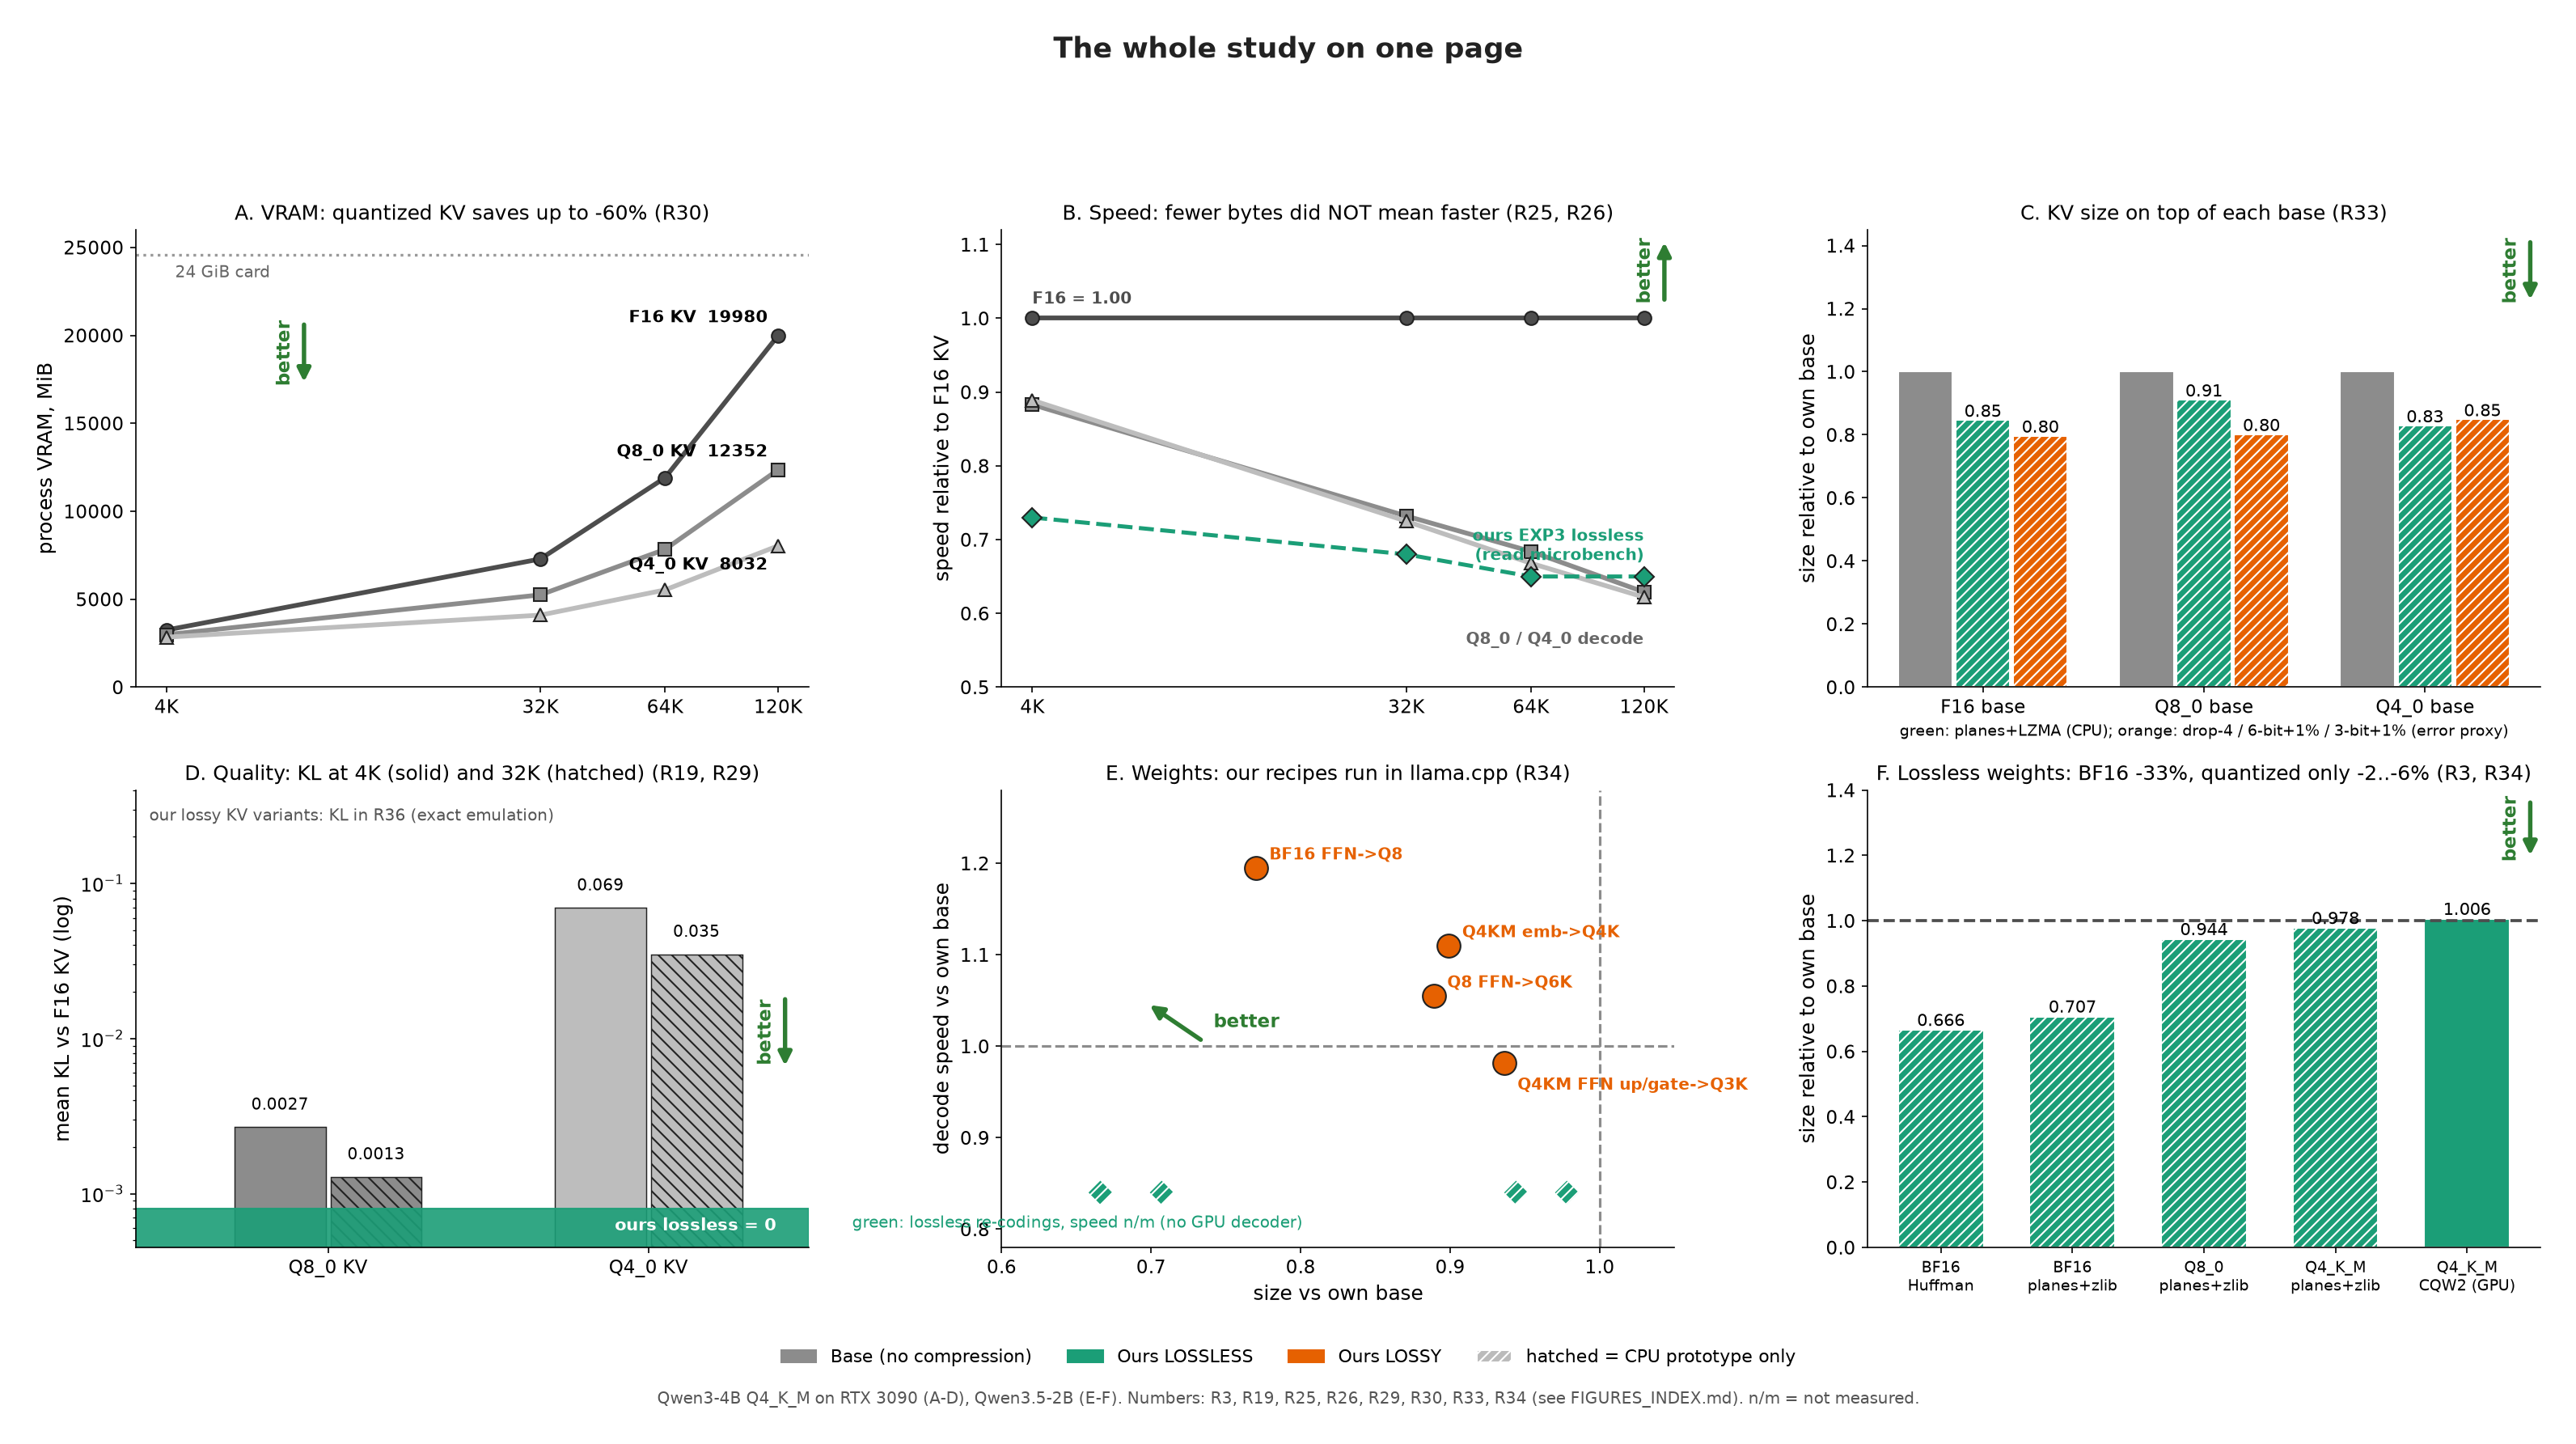
\includegraphics[width=\linewidth]{figures/fig27_dashboard.png}\caption{The study in one page: (A) process VRAM by KV type and context; (B) decode speed of quantized KV and read speed of our lossless EXP3, both against F16; (C) KV size on top of each base; (D) KL of built-in KV types; (E) weight recipes, size against speed; (F) lossless weights. Grey is base, green ours lossless, orange ours lossy, hatched CPU prototype only (R3, R19, R25, R26, R29, R30, R33, R34; KL of our lossy KV variants is in R36, Tables 4.1--4.3).}\end{figure}

\section{Related work}

\begin{itemize}
\item \textbf{Lossless KV (BF16/FP8):} SplitZip 2605.01708 [full*] (BF16 KV exponent entropy 2.89--3.59 bits; a fixed 4-bit code plus an exception stream; 1.31--1.33$\times$; 1.14$\times$ on FP8; decodes on the transfer path, not inside attention). Heilper \& Singer 2508.19263 [full*] (Huffman on KV exponents, mantissas stored raw). TRACE 2509.03377 [full*] (BF16 KV, channel-major grouping, exponent delta, bit planes + zstd/LZ4: 1.81--1.88$\times$ on Llama-3.1-8B, inside a CXL controller). LEXI 2603.15589 [abs] (exponent entropy < 3 bits in BF16 activations and caches).
\item \textbf{Lossless weights:} DFloat11 2504.11651 [abs] (\textasciitilde{}70\% of BF16); ZipServ 2603.17435 (ASPLOS'26) [abs+full*]: TCA-TBE (a 3-bit exponent window code with fallback) and a fused ZipGEMM that beats cuBLAS on RTX 4090/L40S; Tan et al. ISCA'26 2606.15789 [abs+full*] (per-layer order-0 entropy; int4 0.6--1.0 bits; group awq4/sq8 "1.1--1.3$\times$ above entropy bound"); ZipNN 2411.05239, NeuZip 2410.20650, ECF8 2510.02676, Huff-LLM 2502.00922, EntroLLM 2505.02380 [abs].
\item \textbf{Lossy / entropy-coded KV:} KIVI 2402.02750 [abs], KVQuant 2401.18079 [abs] (per-channel K, dense-and-sparse outliers), GEAR 2403.05527 [abs], KVTC 2511.01815 [abs], CacheGen 2310.07240 [abs], Ecco 2505.06901 [abs], D-Quant 2609.19880 [abs], JoLT 2607.12550 [abs], TailorKV 2505.19586 [abs]; FP8 E5M2 KV in vLLM [web]. Low-bit KV on tensor cores: BitDecoding 2503.18773 [abs]; QServe 2405.04532 [abs] (dequantization on CUDA cores costs 20--90\%).
\item \textbf{llama.cpp kernel paths for quantized KV} [gh]: \#29371 (the f16 scratch cost grows with context), \#24166 (scratch sized to allocated KV), \#27796 (q8\_0/q4\_0 slowdowns on RDNA4), \#30790 / PR \#30792 (bs=1 quantized KV drops back to the VEC kernel without K/V reuse across GQA heads), PR \#30202 (on-the-fly dequantization in vec kernels), SYCL PR \#26689.
\item \textbf{Allocation:} PagedAttention 2309.06180, vAttention 2405.04437, kvcached/Prism 2505.04021, Elastic KV 2608.23658 [abs]; llama.cpp PR \#21757 \texttt{--kv-dynamic} [gh].
\item \textbf{Regimes and metrics:} Singh 2609.30854 [abs]; LLM-Viewer 2402.16363 [abs]; Dutta et al. 2407.09141 [abs] (KL and flips as quality metrics).
\end{itemize}

Where we found no numbers, we added some: IEEE F16 KV in llama.cpp (field- and context-level entropy, real
codecs), lossless coding on top of llama.cpp Q8\_0/Q4\_0 blocks, GGUF k-quant entropy with the negative CQW2
format, quality of lossy variants on top of each base through exact emulation, and an ABBA series out to 120K
with per-process VRAM on Windows.

\section{Setup and methods}

RTX 3090 24 GB (WDDM, PCIe Gen3 x16, BAR1 256 MiB, so no Resizable BAR), i7-10700K, 64 GB RAM, CUDA 11.8.
llama.cpp build 11552 (\texttt{23b0202a}) for bench, perplexity and server; our research branch \texttt{cq/kv-compress}
(from \texttt{ed7ac35e}) for the emulation hook; a separate observer build for per-process VRAM. Models:
Qwen3-4B-Q4\_K\_M for the KV studies and Qwen3.5-2B for the weight studies (local BF16, converted and quantized
by us).

\begin{itemize}
\item \textbf{Bases and "ours":} every result is reported as base against base + ours (size, speed, quality relative to that base). Cross-base comparisons are reference only.
\item \textbf{Exact lossy emulation:} an env-gated hook in CUDA \texttt{set\_rows} passes each written K/V row (one token of one layer) through the variant's quantize$\rightarrow$dequantize and stores the dequantized values in an F16 cache. Attention therefore sees exactly what the packed format would decode to, so KL, PPL, tasks and needle are real. Memory and speed of the packed format are not represented (patch in \texttt{release/patches/}).
\item \textbf{Quality:} KL/PPL/top-1 with \texttt{llama-perplexity --kl-divergence} on a fixed corpus (4K: 6 chunks; 32K: one chunk of a tripled corpus, so the second half partly repeats earlier text). A frozen 39-case task suite with a deterministic scorer and greedy decoding. Single-needle retrieval at 4K/32K.
\item \textbf{Speed:} llama-bench at filled depth, ABBA, 6--12 samples per cell, 1 s telemetry. Clean window means all other GPU workloads and GPU applications stopped and no CPU jobs running (R37). Clean-window KV ratios (Q8\_0 / Q4\_0 vs F16): 0.89 / 0.89 at 4K, 0.73 / 0.73 at 32K, 0.64 / 0.63 at 120K (F16: 166 / 91 / 38 tok/s). Weight recipes vs base: BF16 + FFN Q8\_0 1.16--1.18$\times$, Q8\_0 + FFN Q6\_K 1.04--1.06$\times$, Q4\_K\_M + embedding Q4\_K 1.02--1.05$\times$.
\item \textbf{Lossless:} every codec round-trips bit-exactly.
\end{itemize}


\begin{figure}[htbp]\centering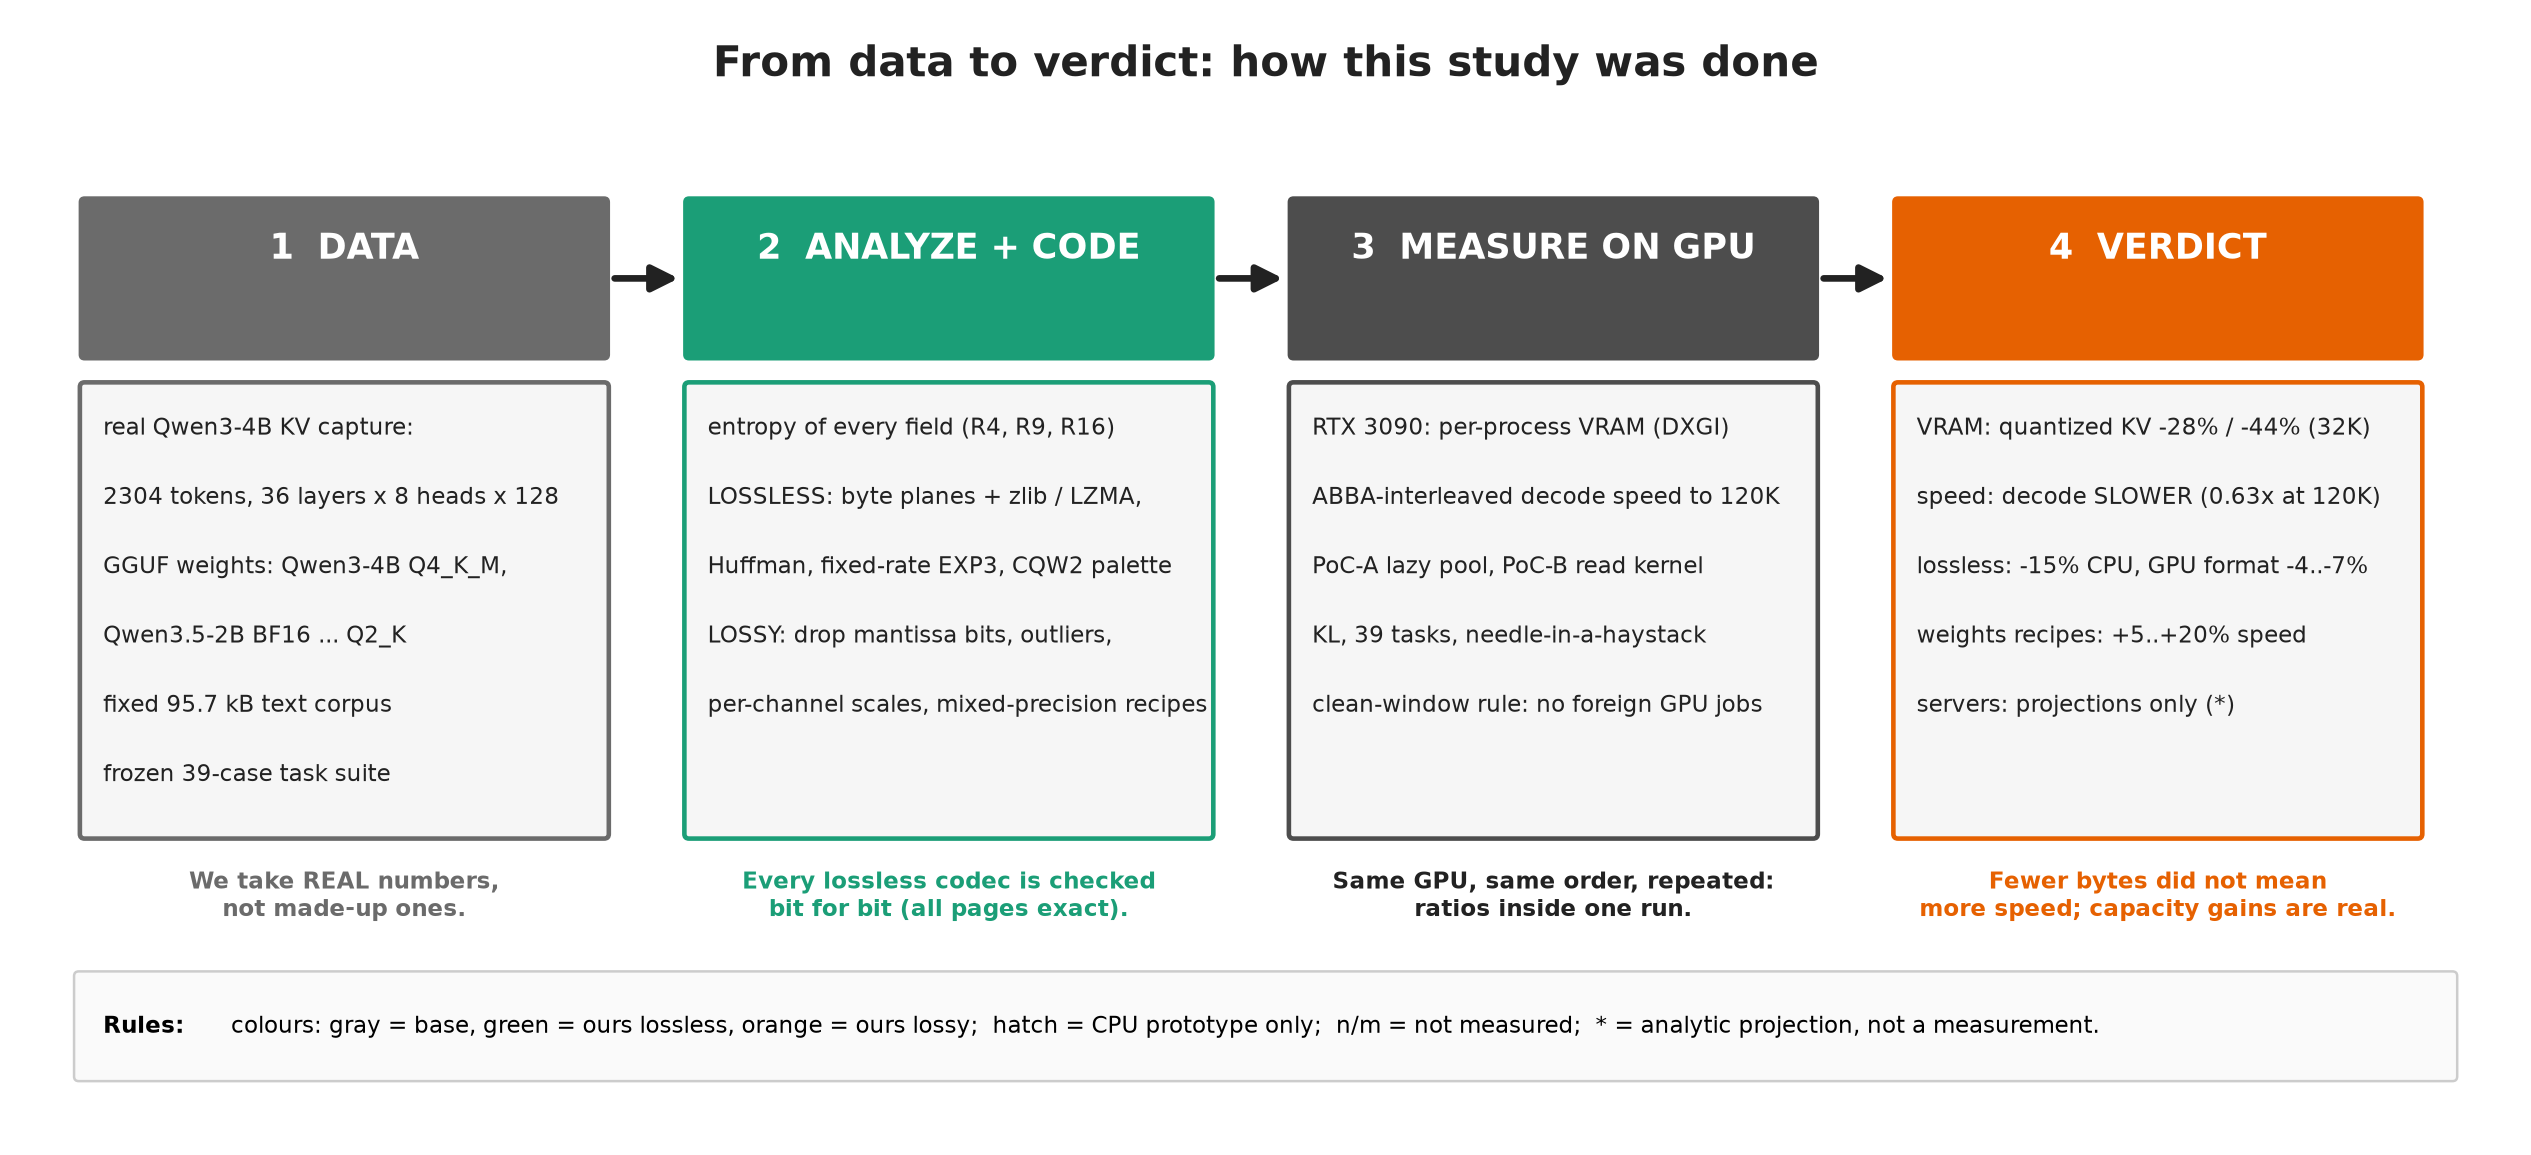
\includegraphics[width=\linewidth]{figures/fig28_pipeline_infographic.png}\caption{How the work went: real KV captures and GGUF weights $\rightarrow$ CPU codecs and exact lossy emulation in llama.cpp $\rightarrow$ GPU measurements in a clean window $\rightarrow$ verdict.}\end{figure}

\section{Results by baseline}

\begin{figure}[htbp]\centering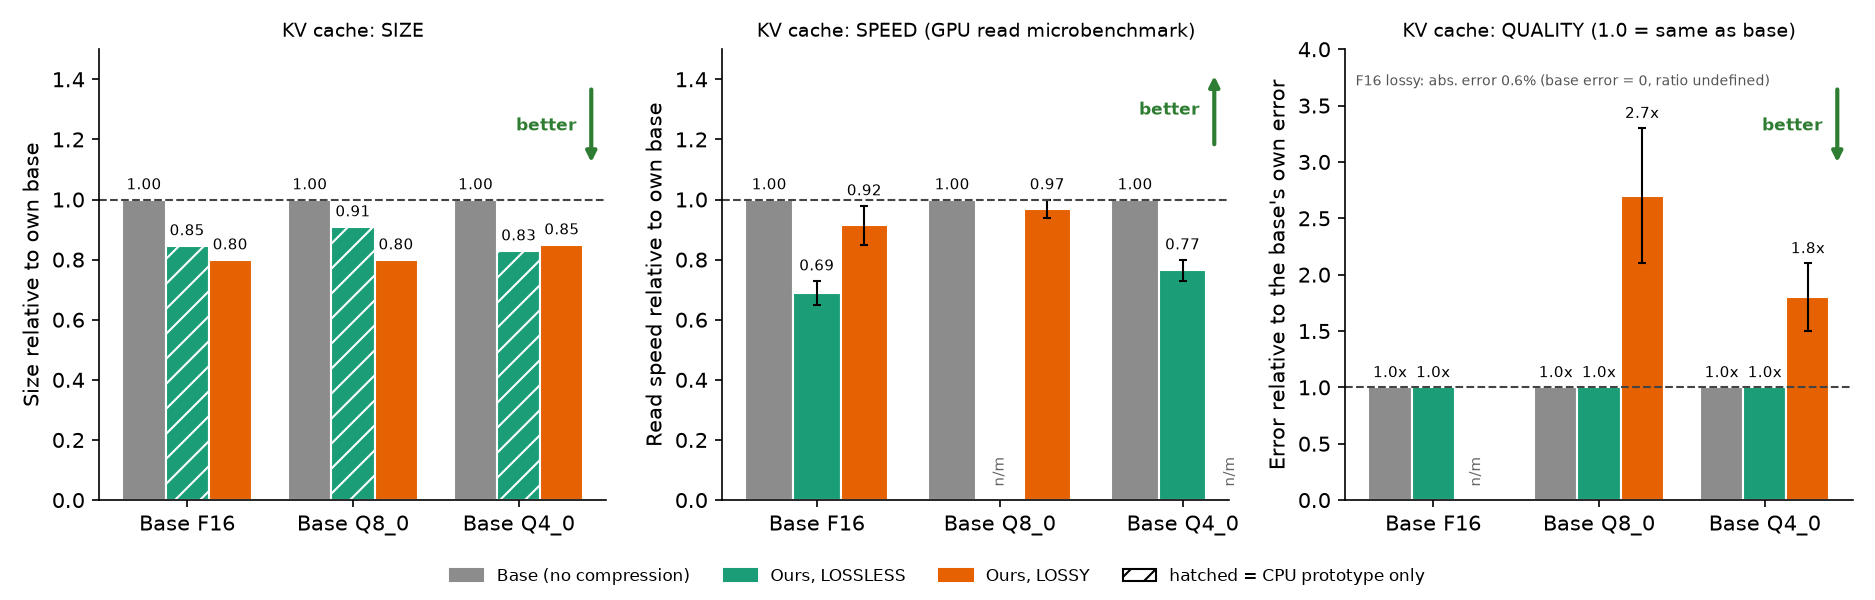
\includegraphics[width=\linewidth]{figures/fig9_kv_three_types.png}\caption{KV cache, base vs base + ours: size, GPU read speed (microbenchmark) and reconstruction error relative to the base (a proxy; measured KL is in Tables 4.1--4.3). n/m = not measured (R26, R33).}\end{figure}

\begin{figure}[htbp]\centering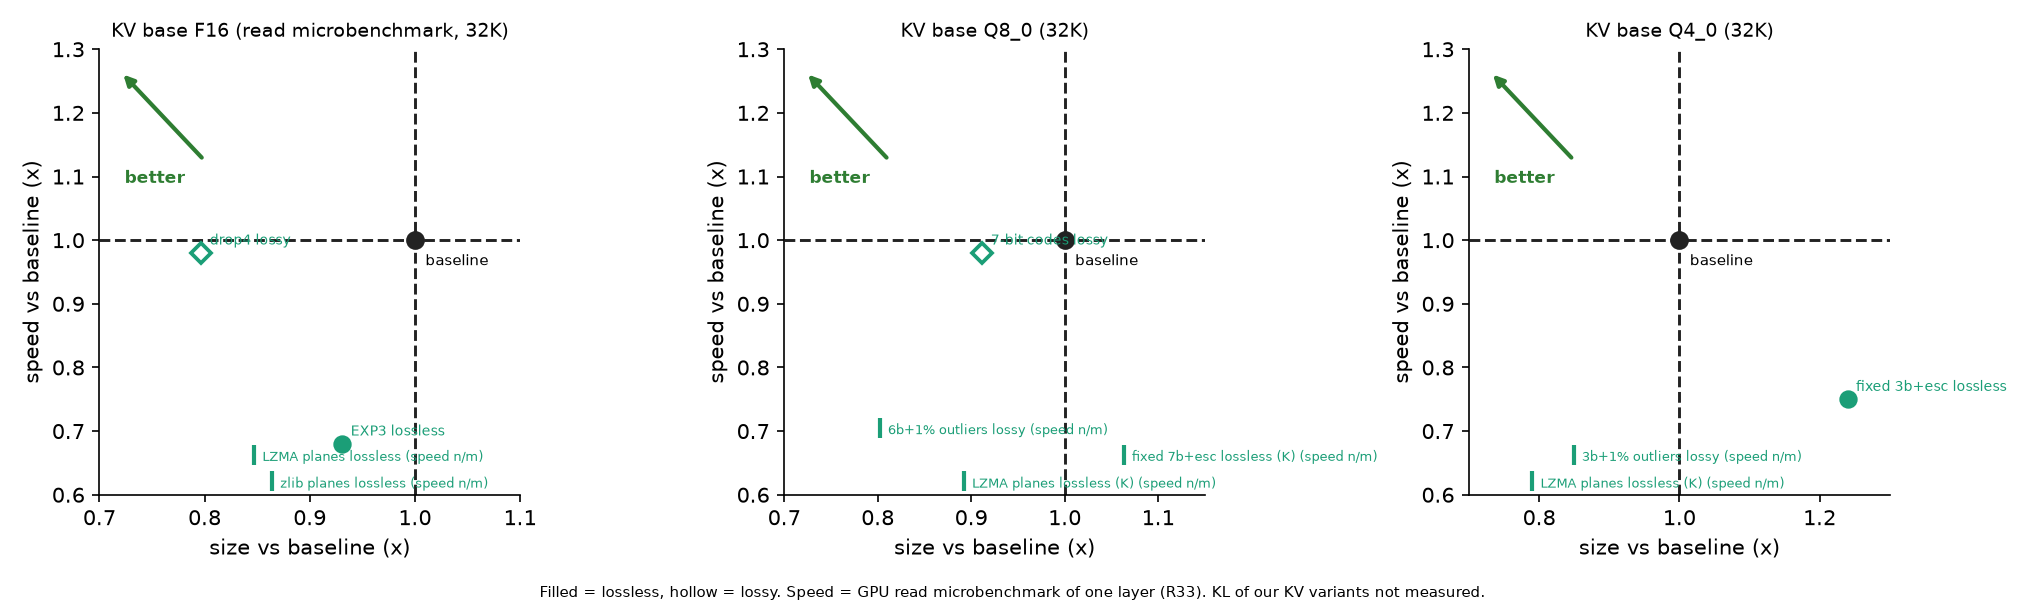
\includegraphics[width=\linewidth]{figures/fig7_kv_base_vs_ours.png}\caption{KV, with each base drawn as a reference line and our variants as points; the arrow points the better way (R33, R36).}\end{figure}

\subsection{KV base F16}

\begin{table}[h]\centering\scriptsize
\resizebox{\linewidth}{!}{%
\begin{tabular}{llllll}
\toprule
Row & Size vs base & Read/decode speed vs base & Quality vs F16 KV (4K / 32K) & Status &  \\
\midrule
F16 (base) & 1.00 & 1.00 & --- & M &  \\
+ lossless, context estimate (exp \textbackslash{} & prev, channel) & 0.827 (K) / 0.840 (V) & --- & exact & M (estimate, E1) \\
+ lossless, TRACE-style bit planes + zstd-19, G=16 & 0.842 / 0.863 & not measured on GPU & exact & M (CPU codec, E1) &  \\
+ lossless, byte planes + LZMA & 0.847 & not measured on GPU & exact & M (CPU codec) &  \\
+ lossless, fixed-rate exponent code ($\approx$ ZipServ TCA-TBE / SplitZip style) & 0.93--0.96 & read 0.65--0.73$\times$ (non-fused scalar kernel) & exact & M &  \\
+ lossy: drop 2 mantissa bits (14 b) & 0.875 & not measured & KL 0.0025 / 0.0012; tasks 25/39 (= F16); needle 10/10 & M &  \\
+ lossy: drop 4 mantissa bits (12 b, $\approx$ FP8 E5M2-like precision) & 0.75 (0.80 packed) & read 0.85--0.98$\times$ & KL 0.0027 / 0.0026; tasks 25/39; needle 10/10 & M &  \\
\bottomrule
\end{tabular}}
\end{table}

The context estimate holds at 0.828--0.830 (K) and 0.841--0.843 (V) over three texts (code, English, Russian)
and about 4K and 30K tokens, and the TRACE-like codec at 0.835--0.842 (K) and 0.862--0.863 (V) (R41). Storing
the same activations as \textbf{BF16 KV} gives 0.640--0.641 / 0.654--0.655 (estimate) and 0.654--0.656 / 0.676--0.677
(codec): BF16 has three fewer noise mantissa bits (\S{}6, E4).

\subsection{KV base Q8\_0}

\begin{table}[h]\centering\scriptsize
\resizebox{\linewidth}{!}{%
\begin{tabular}{lllll}
\toprule
Row & Size vs base & Speed vs base & Quality: KL vs F16 (4K / 32K); KL vs own base & Status \\
\midrule
Q8\_0 (base; real type) & 1.00 & decode vs F16 0.88 / 0.73 / 0.63 at 4K / 32K / 120K & 0.0027 / 0.0013; tasks 25/39 & M \\
+ lossless, split planes + LZMA & 0.892 (K) / 0.931 (V) & not measured on GPU & exact & M (CPU) \\
+ lossless, fixed-rate 7-bit + escape & 1.06 / 1.11 (larger) & --- & exact & M (negative) \\
+ lossy: 7-bit codes & 0.912 & read 0.94--1.00$\times$ & 0.0029 / 0.0028; vs base 0.0030 / 0.0027; tasks 25/39 & M \\
+ lossy: 6-bit + 1\% outliers exact & 0.802 & not measured & 0.0028 / 0.0018; vs base 0.0030 / 0.0016; tasks 25/39 & M \\
\bottomrule
\end{tabular}}
\end{table}

\subsection{KV base Q4\_0}

\begin{table}[h]\centering\scriptsize
\resizebox{\linewidth}{!}{%
\begin{tabular}{lllll}
\toprule
Row & Size vs base & Speed vs base & Quality: KL vs F16 (4K / 32K); vs own base & Status \\
\midrule
Q4\_0 (base; real type) & 1.00 & decode vs F16 0.89 / 0.73 / 0.62 & 0.069 / 0.035; tasks 21/39 & M \\
Q4\_0 format, emulated (same values, F16 attention path) & 1.00 & --- & \textbf{0.0080 / 0.0051}; tasks 24/39 & M \\
+ lossless, split planes + LZMA & 0.790 (K) / 0.869 (V) & not measured on GPU & exact & M (CPU) \\
+ lossless, fixed-rate 3-bit + escape & 1.17--1.25 (larger) & read 0.73--0.80$\times$ & exact & M (negative) \\
+ lossy: 4-bit + 1\% outliers exact & 1.071 & not measured & \textbf{0.0063 / 0.0037}; vs base 0.011 / 0.0066; tasks 25/39 & M \\
+ lossy: 3-bit + 1\% outliers exact & 0.849 & not measured & 0.023 / 0.012; vs base 0.029 / 0.015; tasks 25/39 & M \\
\bottomrule
\end{tabular}}
\end{table}

How to read this. \textbf{Correction (R44, R45):} the emulation in this table quantized V only (the fused
rope+set\_rows path wrote K directly), so the "format" rows understate the loss. With K and V both quantized,
the emulated Q4\_0 format costs KL 0.116 without the attention rotation, the same as the real type without
rotation; llama.cpp's default rotation brings the real q4\_0 to 0.068. We withdraw the statement that "the
real q4\_0 path costs nine times more than the format". The original reading is kept below. At the format
level Q4\_0 loses little: its emulated values cost KL 0.008 at 4K. llama.cpp's real q4\_0 KV path costs nine
times more (0.069) and loses 4 tasks. Keeping 1\% of values exact puts 4-bit KV closer to F16 than plain Q4\_0
is (0.0063 vs 0.0080). Going down to 3 bits with outliers costs about 3$\times$ the base KL. Every lossy variant we
built keeps task accuracy at F16's 25/39, and needle retrieval stays perfect. Per-channel K scales
(KIVI/KVQuant) could not be emulated row by row and are not measured here; their proxy is in R13.


\begin{figure}[htbp]\centering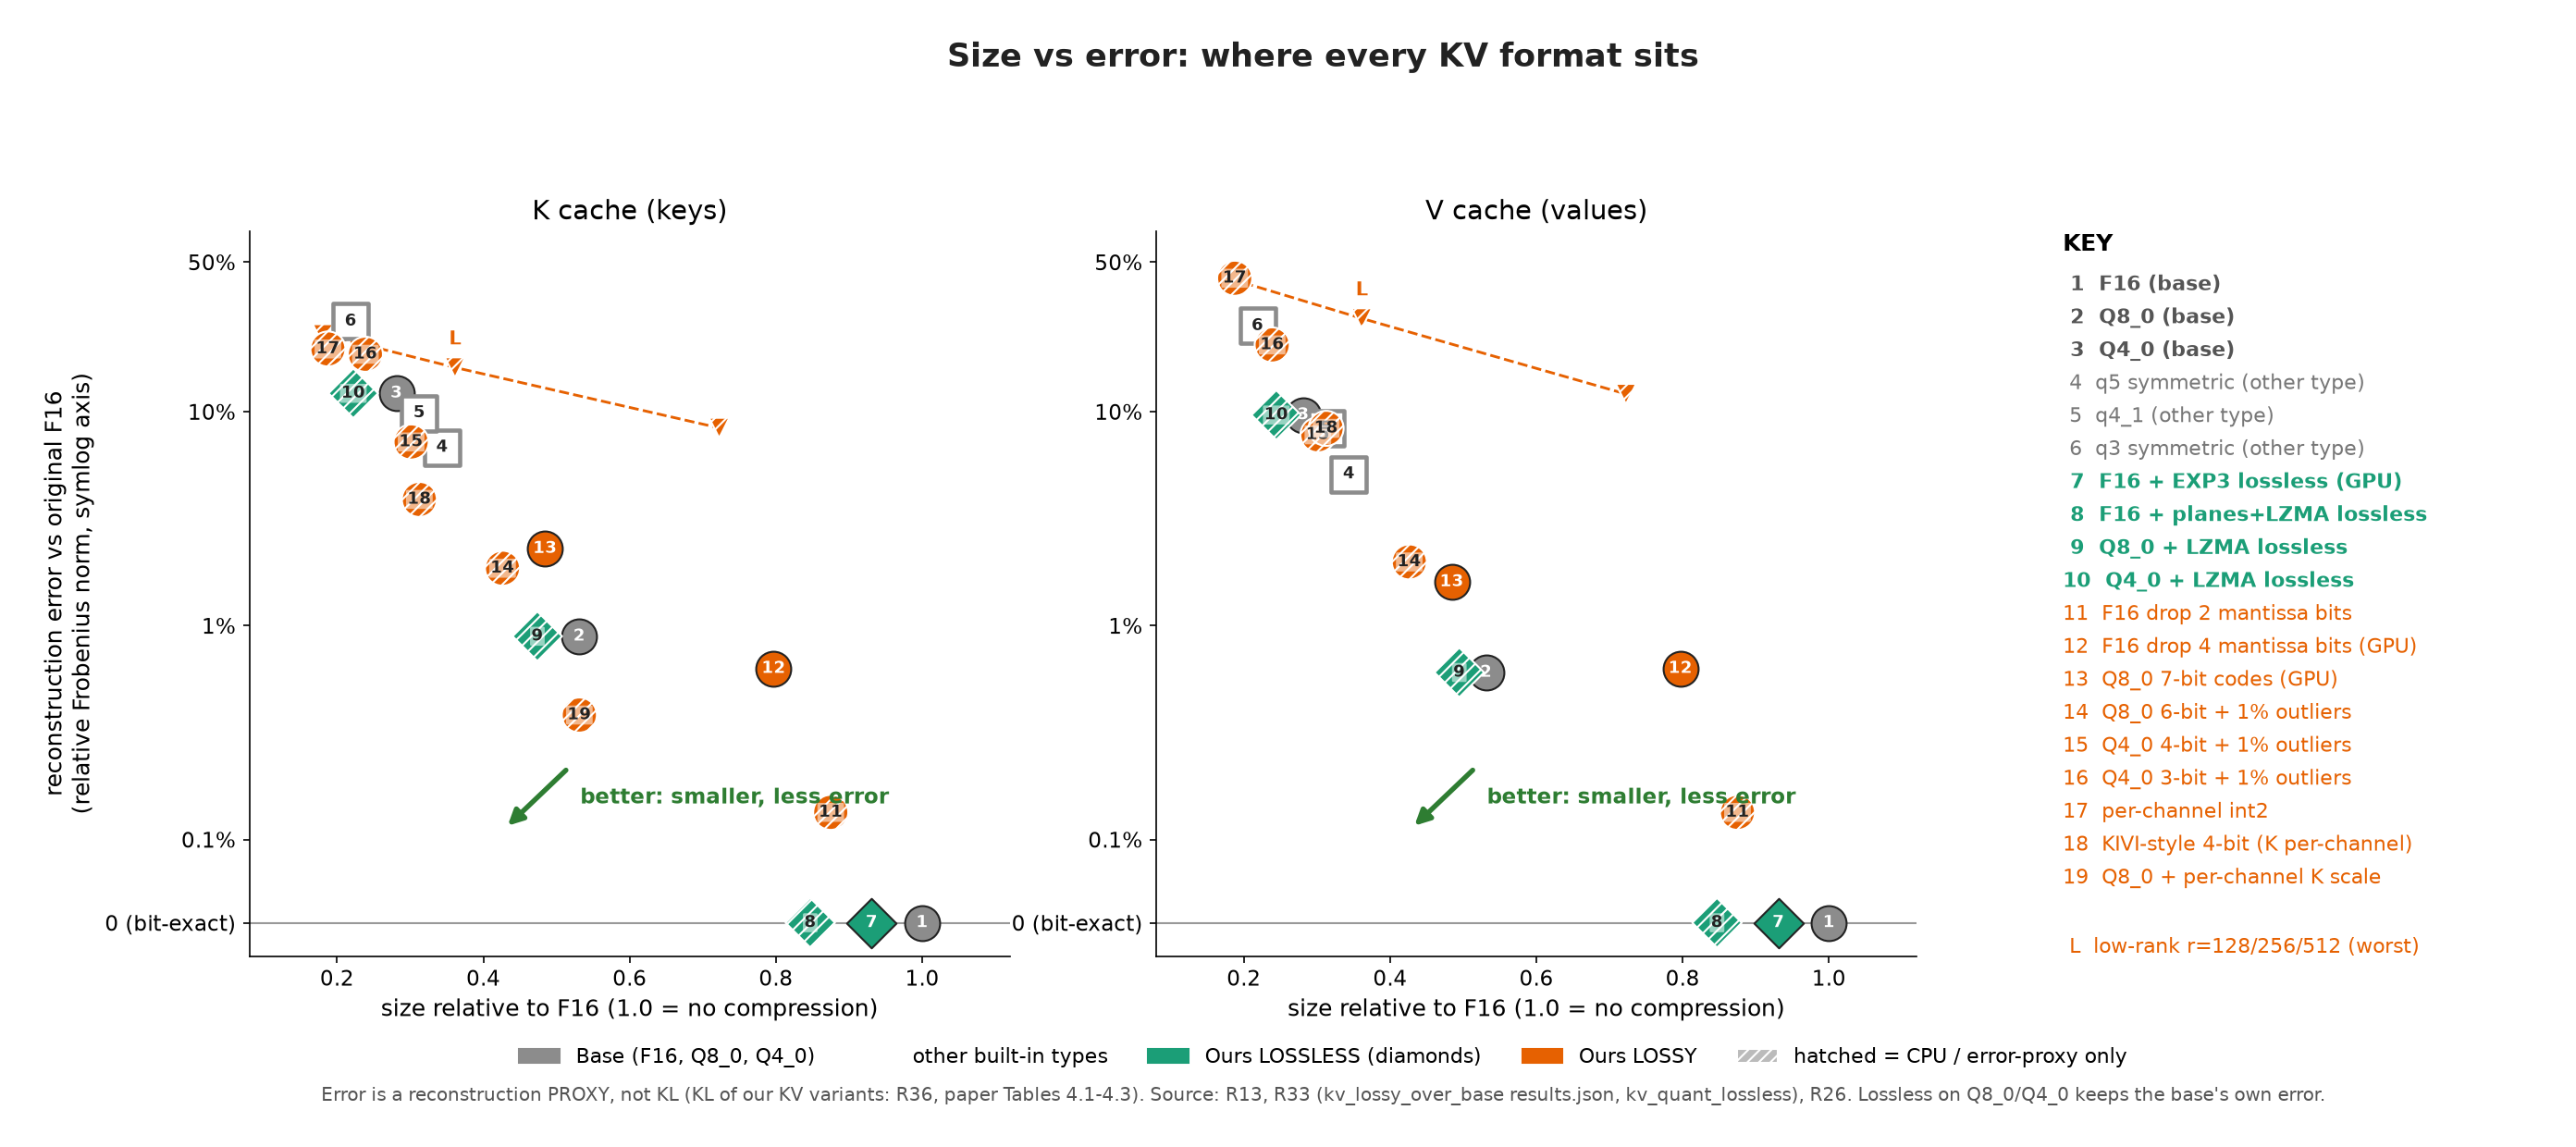
\includegraphics[width=\linewidth]{figures/fig14_pareto_size_vs_error.png}\caption{KV size against reconstruction error for every format, K and V (proxy error, not KL). Lossless coding keeps the error of its base and moves it left; lossy variants trade error for size (R13, R33).}\end{figure}

\subsection{Weight bases (Qwen3.5-2B; llama.cpp decode; quality = KL vs Q8\_0, top-1, tasks)}

\begin{table}[h]\centering\scriptsize
\resizebox{\linewidth}{!}{%
\begin{tabular}{llllll}
\toprule
Base & + lossless (CPU, no GPU decoder) & + lossy recipe (ours as data point; known practice) & size & decode vs base (d=0 / 4K) & quality base $\rightarrow$ ours \\
\midrule
BF16 & 0.666 (exponent Huffman, as DFloat11); fixed-rate 11-bit exponent code 0.716, but GEMV 0.685$\times$ of BF16 in our non-fused scalar kernel (R38) & FFN $\rightarrow$ Q8\_0 & 0.770 & 1.160 / 1.181 & KL 0.0013 $\rightarrow$ 0.0013; tasks 27 $\rightarrow$ 28 \\
Q8\_0 & 0.944 (split + zlib) & FFN $\rightarrow$ Q6\_K & 0.889 & 1.043 / 1.058 & 0 $\rightarrow$ 0.0046; 28 $\rightarrow$ 29 \\
Q4\_K\_M & 0.978; CQW2 palette 1.006 (larger) & embedding/output $\rightarrow$ Q4\_K & 0.899 & 1.024 / 1.046 & 0.060 $\rightarrow$ 0.077; 27 $\rightarrow$ 28 \\
Q4\_K\_M & --- & FFN up/gate $\rightarrow$ Q3\_K & 0.936 & 0.982 / 0.950 (slower) & 0.060 $\rightarrow$ 0.125; 27 $\rightarrow$ 25 \\
\bottomrule
\end{tabular}}
\end{table}

Speeds come from the clean-window rerun (R37, 6 samples); the FFN $\rightarrow$ Q3\_K row is from the near-clean run (R34).
A task difference of 1--2 cases out of 39 means nothing (sign test p $\geq$ 0.25). We could not re-check the recipe
effect on a second model, because no other high-precision checkpoint is available locally.


\begin{figure}[htbp]\centering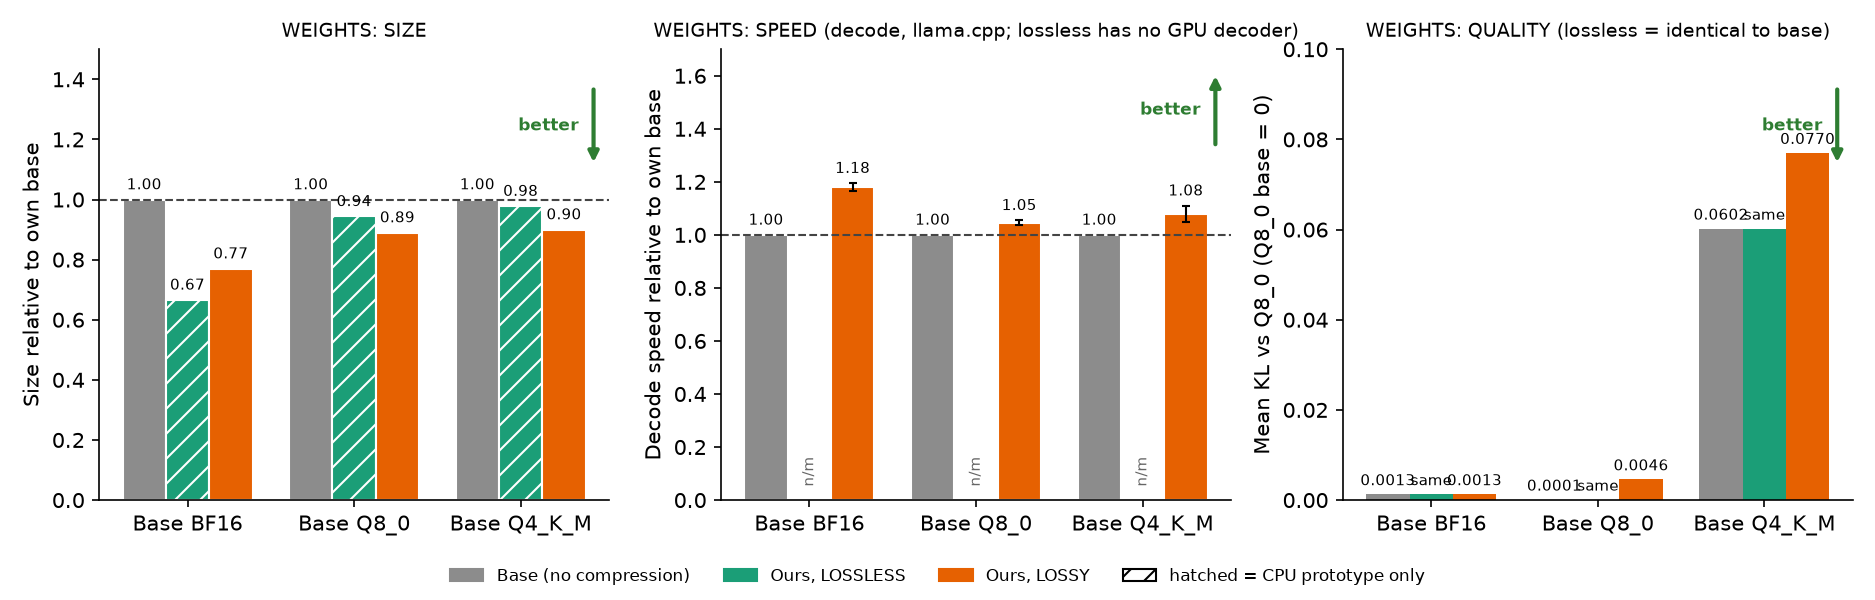
\includegraphics[width=\linewidth]{figures/fig10_weights_three_types.png}\caption{Weights, base vs base + ours: size, decode speed in llama.cpp and KL vs Q8\_0 (R34). Lossless re-codings have no GPU decoder, so their speed is n/m.}\end{figure}

\begin{figure}[htbp]\centering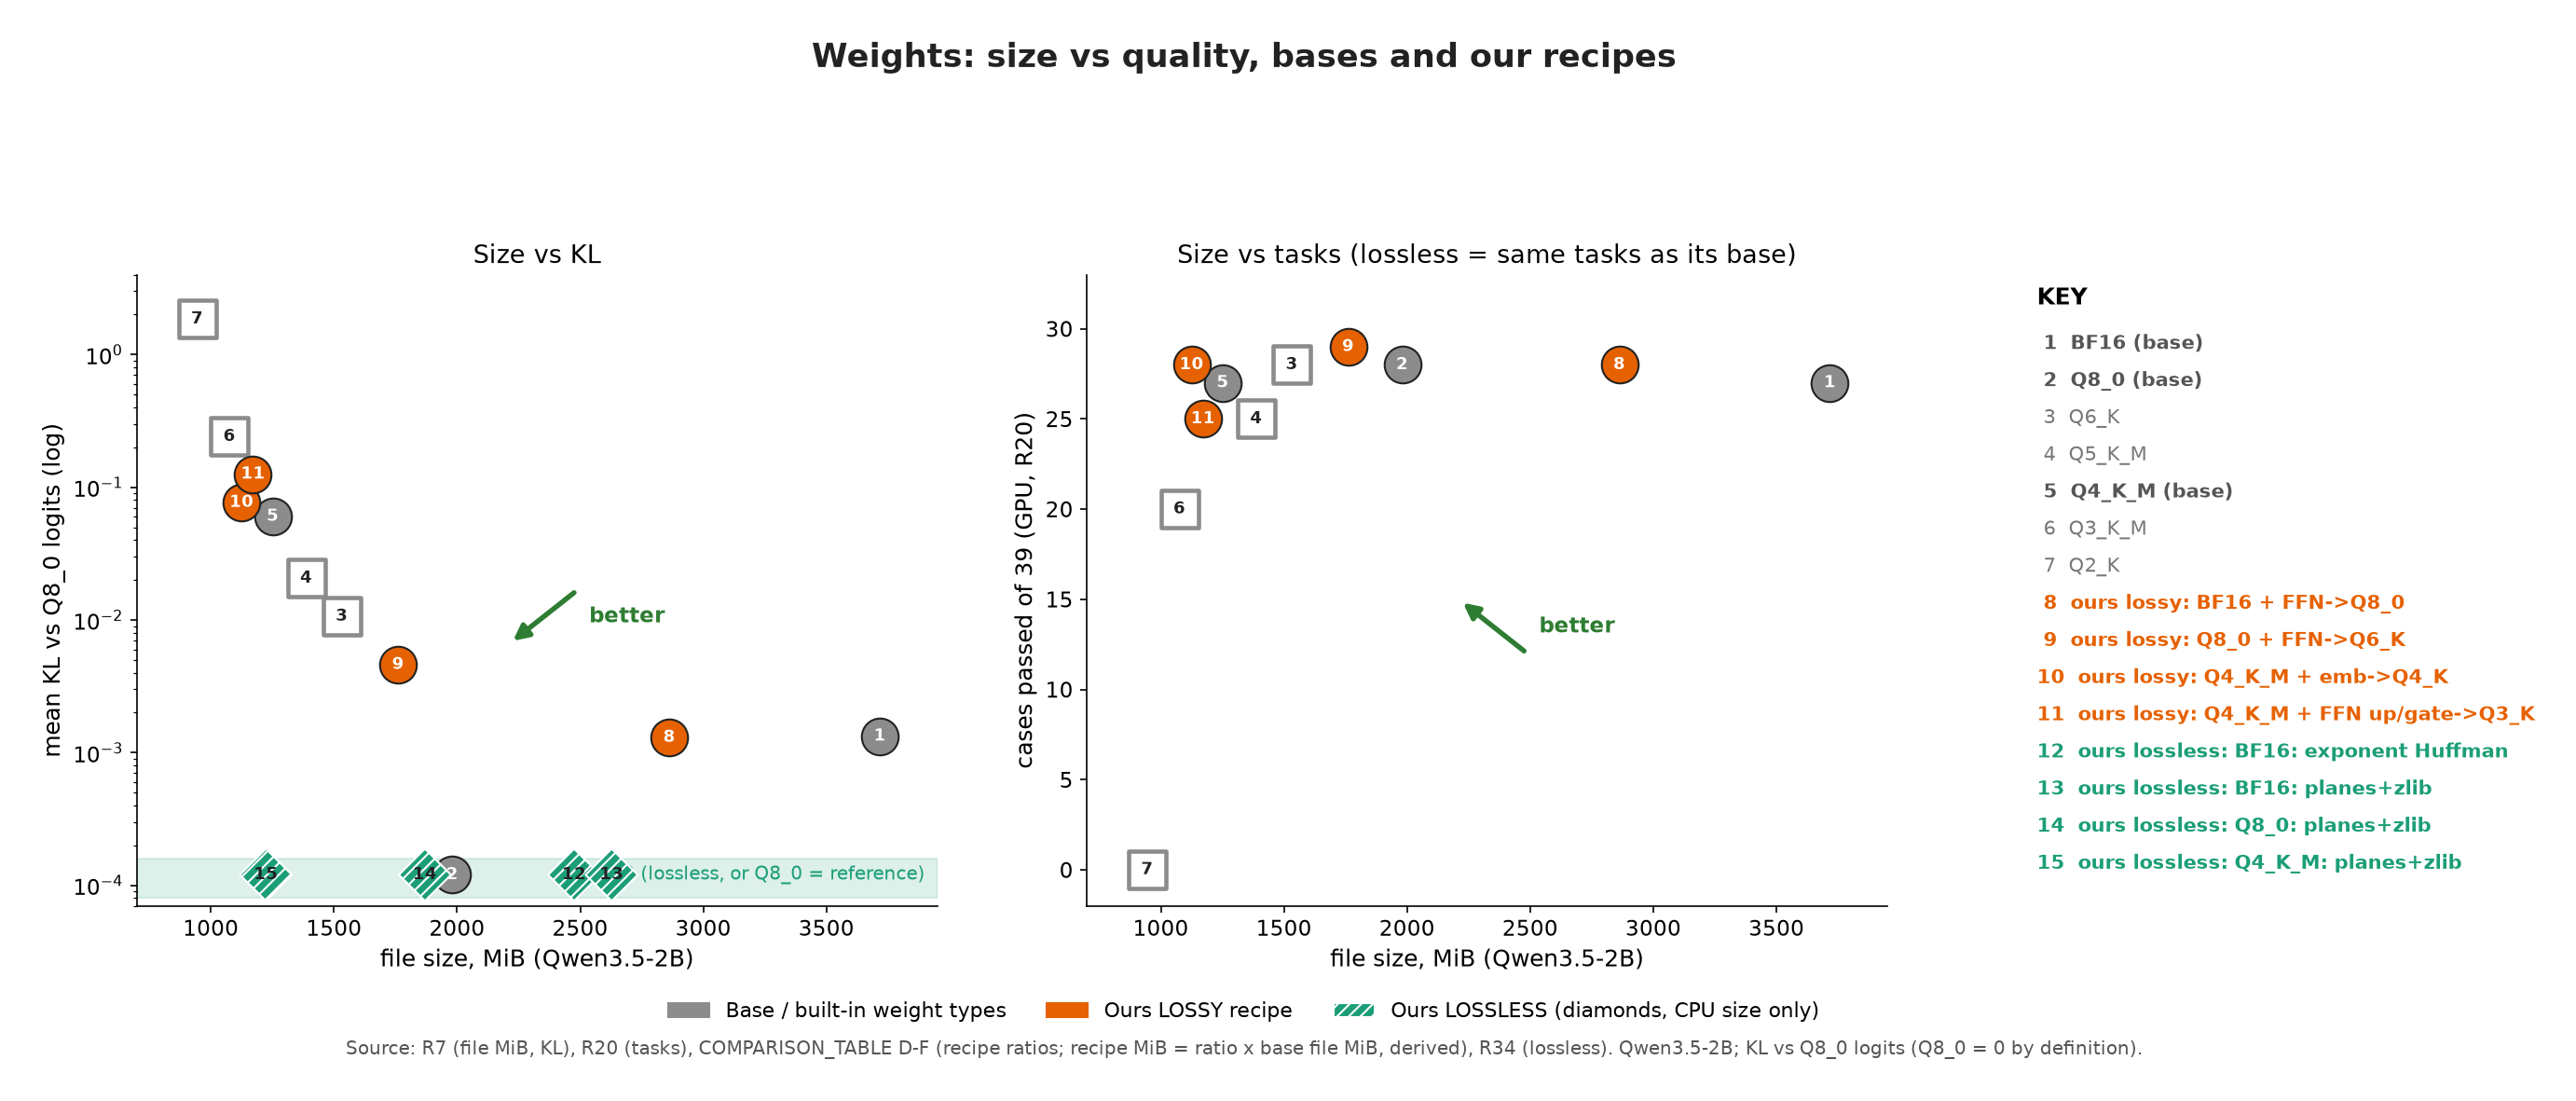
\includegraphics[width=\linewidth]{figures/fig24_weights_size_vs_quality.png}\caption{Weights: size against KL and tasks for built-in types, our mixed-precision recipes and lossless re-codings (R7, R20, R34).}\end{figure}

\begin{figure}[htbp]\centering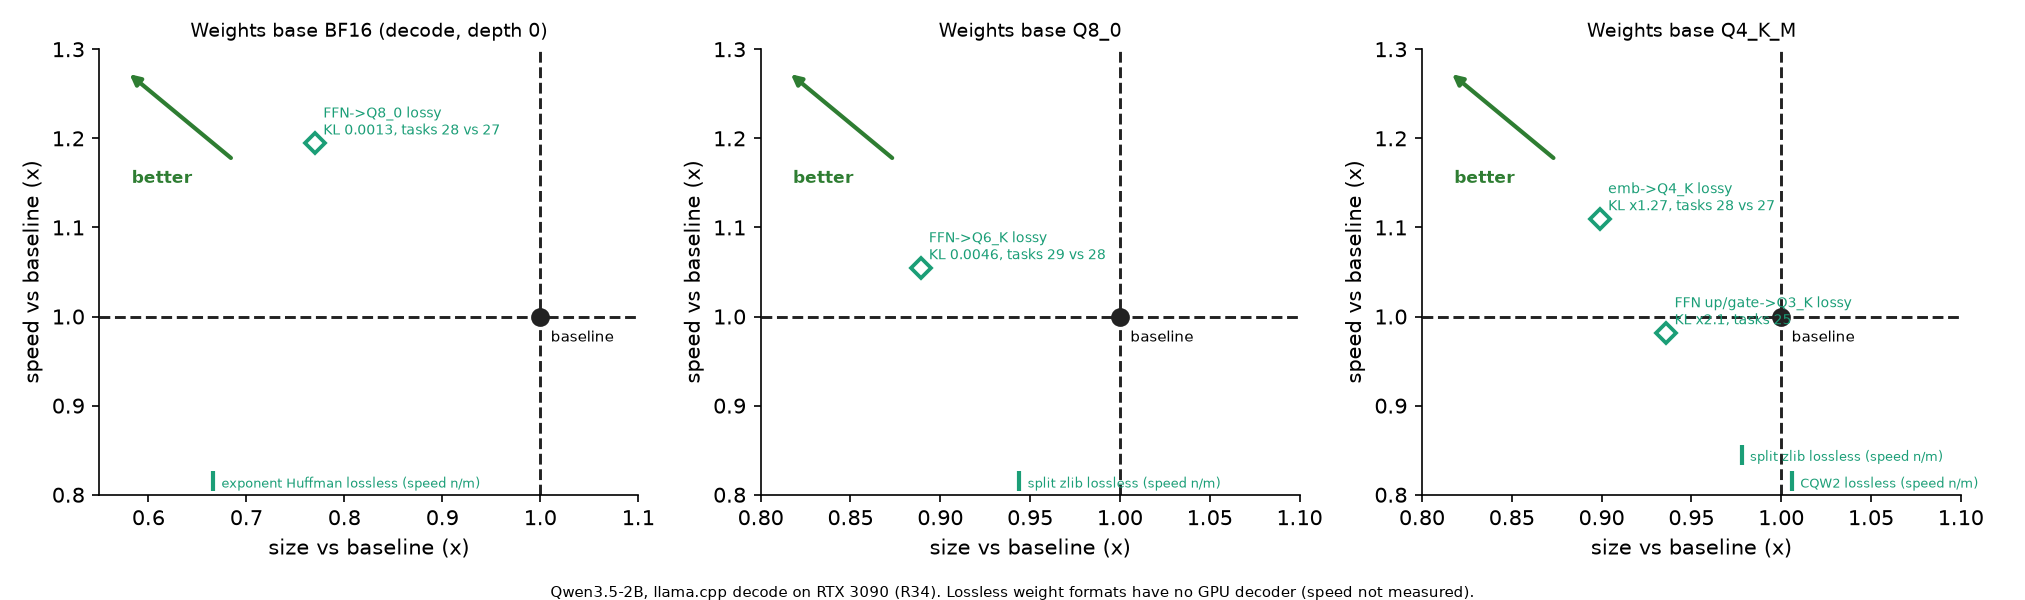
\includegraphics[width=\linewidth]{figures/fig8_weights_base_vs_ours.png}\caption{Weights, with each base as a reference line and our recipes as points (R34; speeds of the clean rerun are in R37).}\end{figure}

\subsection{Combos (weights + KV; Qwen3.5-2B, decode at 4K / 32K)}

Q8\_0 + Q8\_0 KV runs at 218.3 / 194.4 tok/s, and with our Q8\_0 recipe 1.01$\times$ of that. Q4\_K\_M + Q4\_0 KV goes
from 256.4 / 225.0 to 1.06 / 1.03$\times$ with our Q4\_K\_M recipe. Combos of lossless KV with lossless weights were
analytic here; Section 7 measures them with real kernels (Table 7.1).

\begin{figure}[htbp]\centering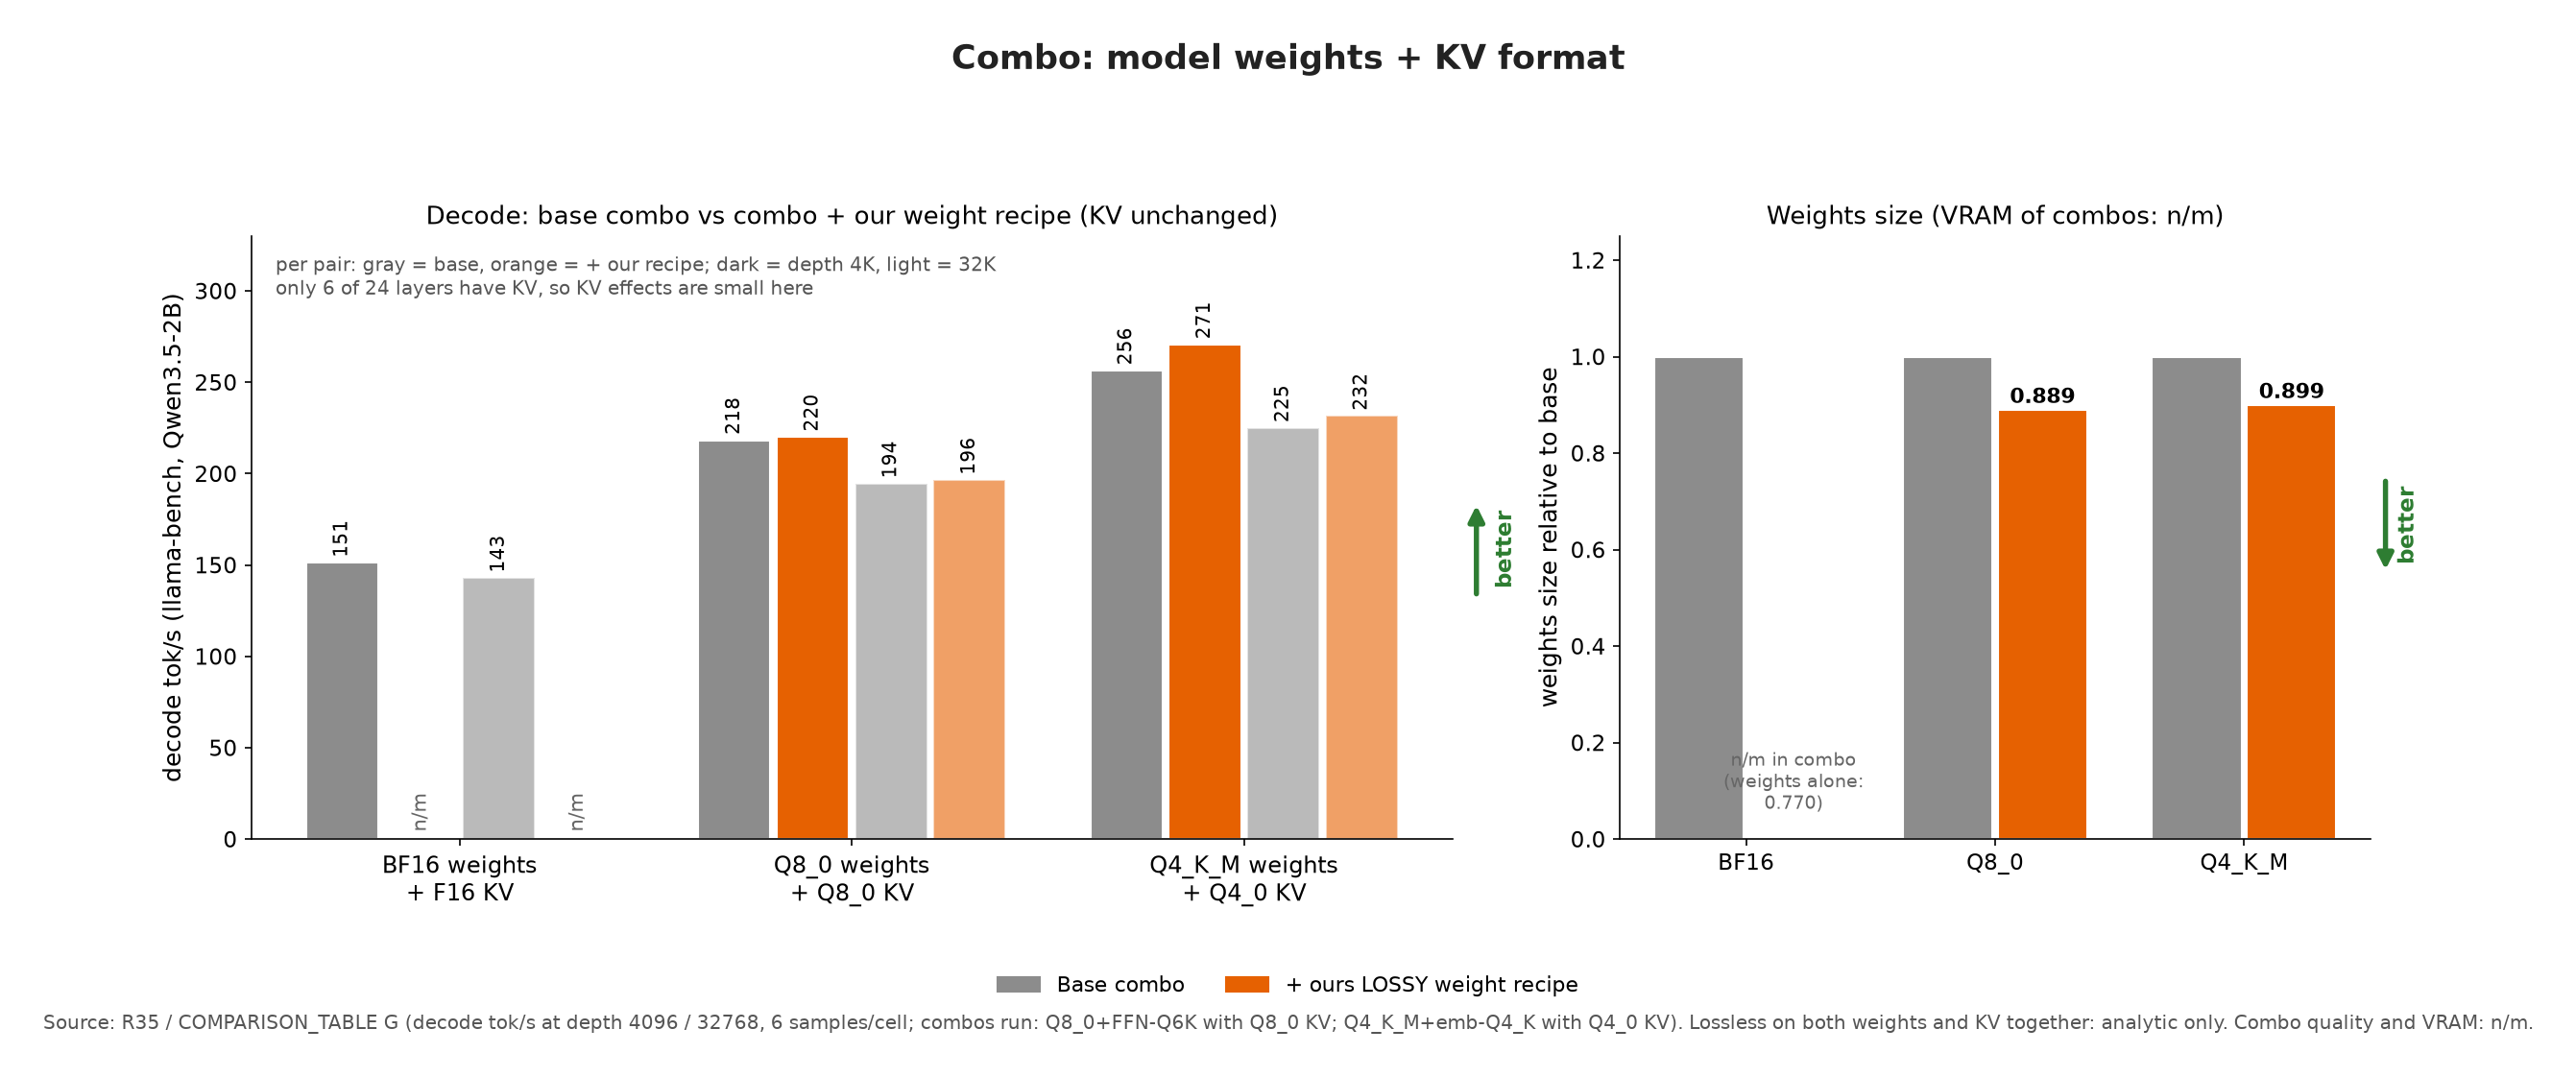
\includegraphics[width=\linewidth]{figures/fig26_combo_weights_plus_kv.png}\caption{A weight recipe on top of a KV format: base combo vs combo + recipe, decode at 4K and 32K (R35). VRAM of combos and of the lossless combo is not measured.}\end{figure}
\section{Where the predicted gains went (diagnostics)}

\begin{itemize}
\item \textbf{F16 KV lossless:} only the exponent compresses (2.4--2.9 of 5 bits). The mantissa is noise (10.0 of 10). F16 therefore has at most about 2.7 bits of redundancy, against 5.7 for BF16 KV of the same activations (R41). That is why a fixed-rate exponent code saves a mere 4--7\% and cannot pay for its decode: 2.0 ps per element in our kernel, against 3.8 ps per element to read F16 at 530 GB/s. On top of Q4\_0 a decoder would have to cost under about 0.22 ps per element to win. Ours is about 10$\times$ too expensive.
\item \textbf{Quantized KV decode in llama.cpp:} at bs=1, quantized KV goes through the VEC kernel, which does not reuse K/V across GQA heads, or through an f16 scratch conversion (\#30790, \#29371). The compute buffer we measured (23.6 $\rightarrow$ 516.6 MiB from 4K to 120K for quantized KV, against 20--49 MiB for F16) is that scratch (\#24166). E2 measures what the proposed fixes recover (R39, clean window, base vs PR builds, ABBA): PR \#30202 (on-the-fly dequantization in vec kernels) speeds q8\_0 decode by 26\% at 32K and 36\% at 120K, lifting q8\_0/F16 from 0.73 to 0.92 at 32K and from 0.64 to 0.86 at 120K. q4\_0 gets back about a third of its gap. PR \#30792 does nothing on this CUDA GPU. Quantized KV is still slower than F16 at long context. (Figure 10)
\item \textbf{Capacity:} llama.cpp reserves KV memory for the full \texttt{-c}; filled and allocated differ by only 14--16 MiB. Lazy allocation fixes it (known work: vAttention, kvcached, PR \#21757).
\end{itemize}


\begin{figure}[htbp]\centering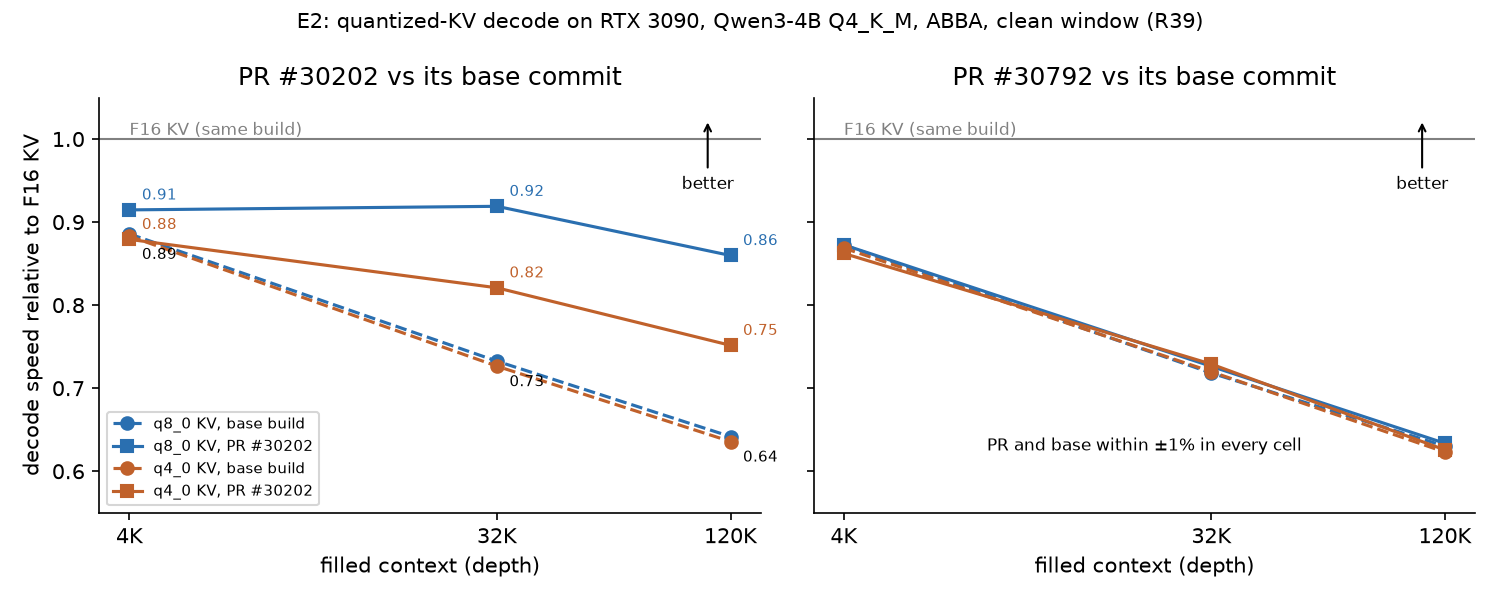
\includegraphics[width=\linewidth]{figures/fig50_e2_llamacpp_prs.png}\caption{E2: decode speed of quantized KV relative to F16 KV in the same build, base commit vs PR build, ABBA, clean window (R39). PR \#30202 lifts q8\_0 from 0.64 to 0.86 of F16 at 120K; PR \#30792 changes nothing on the RTX 3090.}\end{figure}

\begin{figure}[htbp]\centering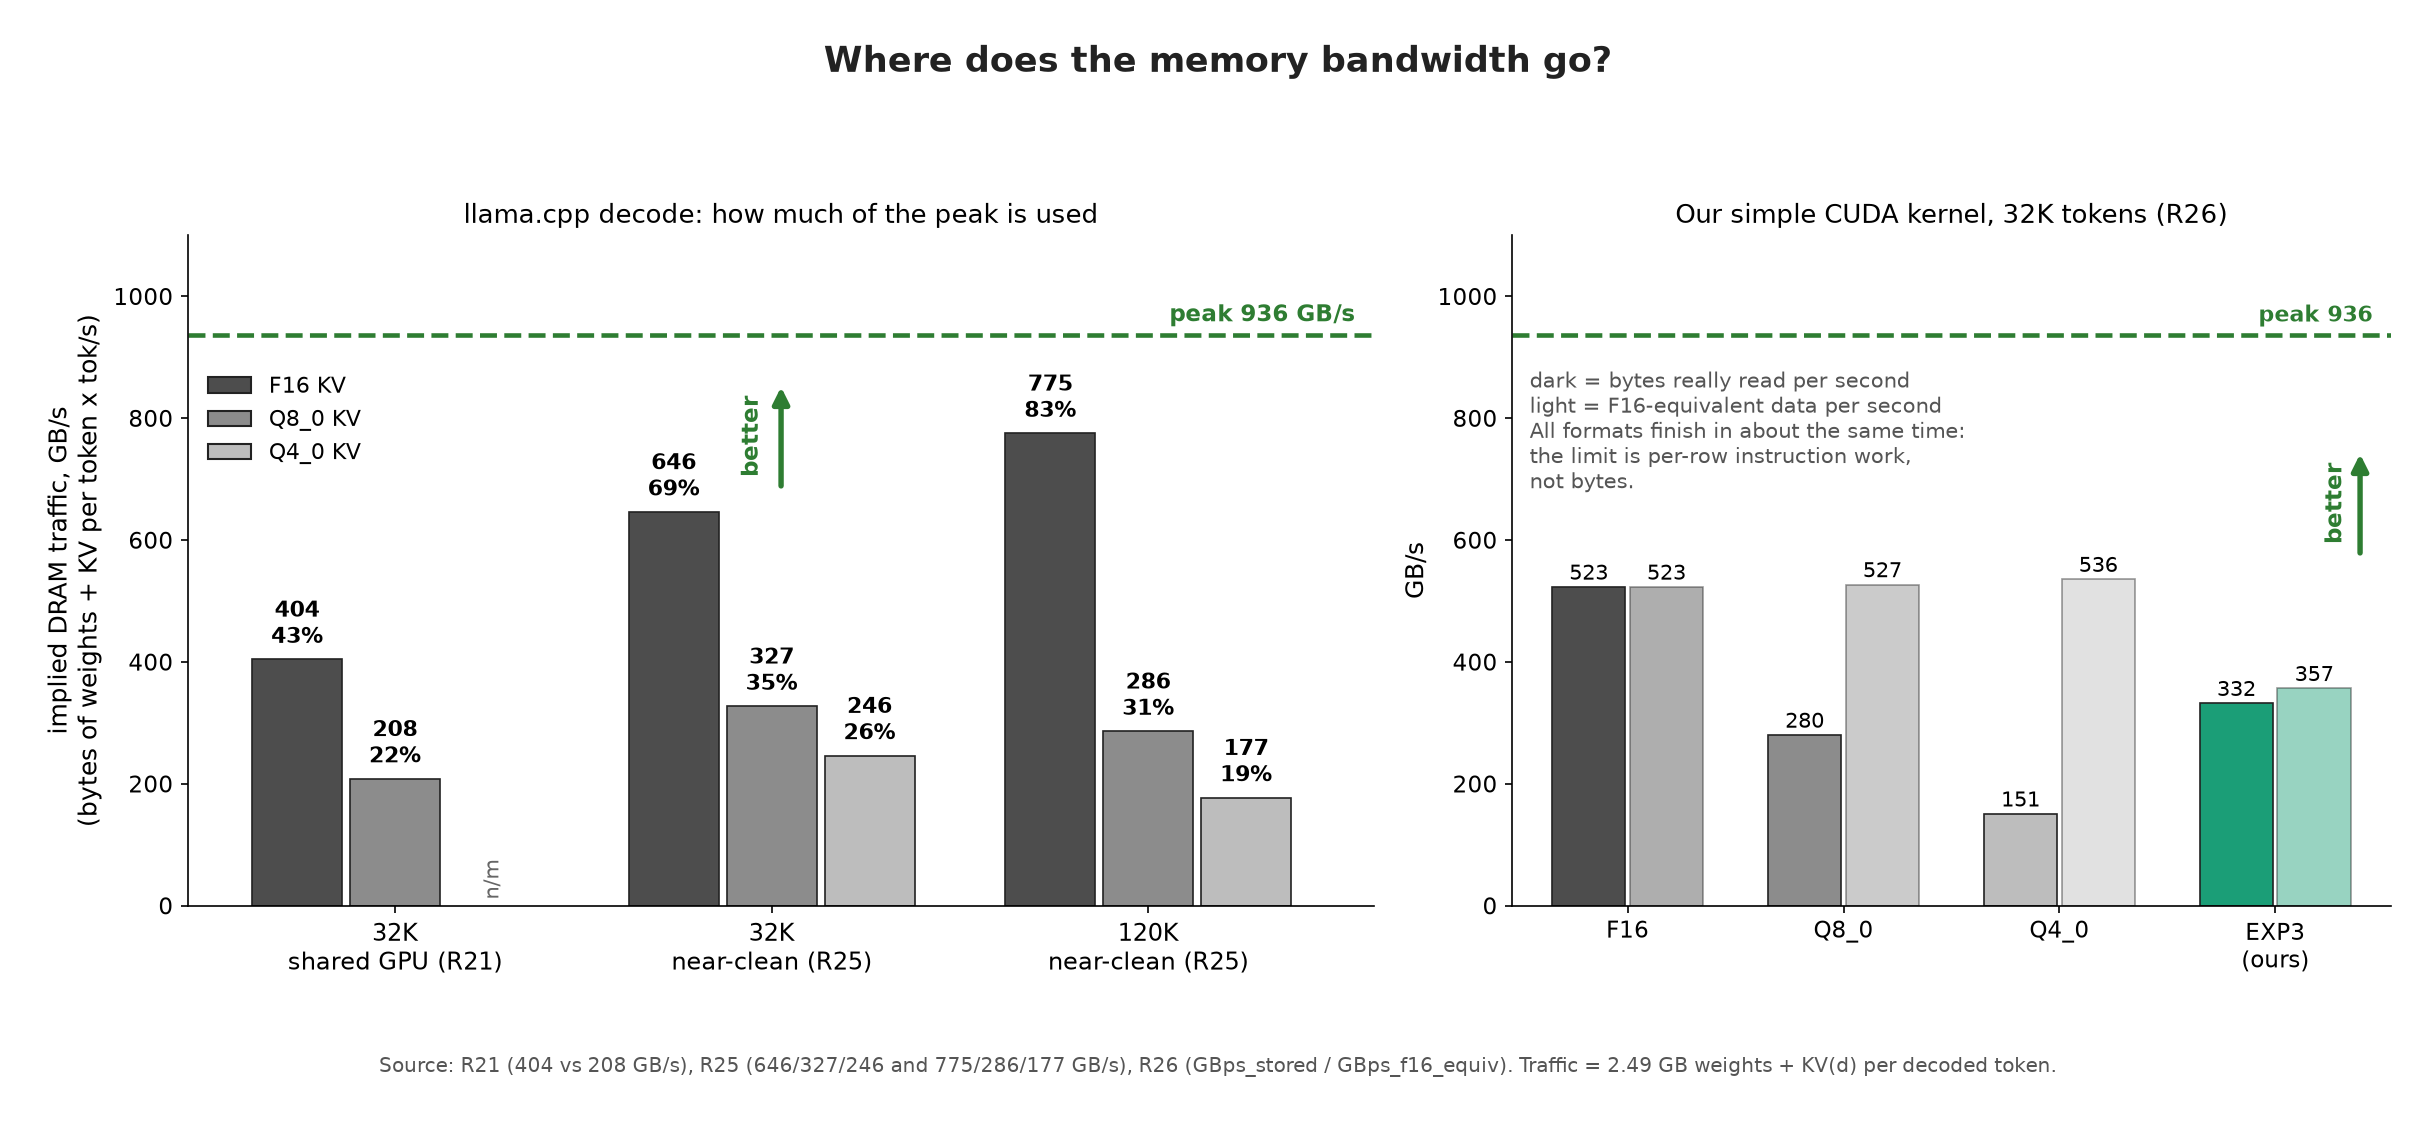
\includegraphics[width=\linewidth]{figures/fig20_bandwidth_real_vs_peak.png}\caption{Implied memory traffic against the 936 GB/s peak. At 120K the F16 path reaches 83\%, Q8\_0 31\% and Q4\_0 19\% (R21, R25), so the quantized path is limited by its kernel, not by bytes. Our scalar read kernel reaches about 57\% on F16 and gains nothing from fewer bytes (R26).}\end{figure}

\begin{figure}[htbp]\centering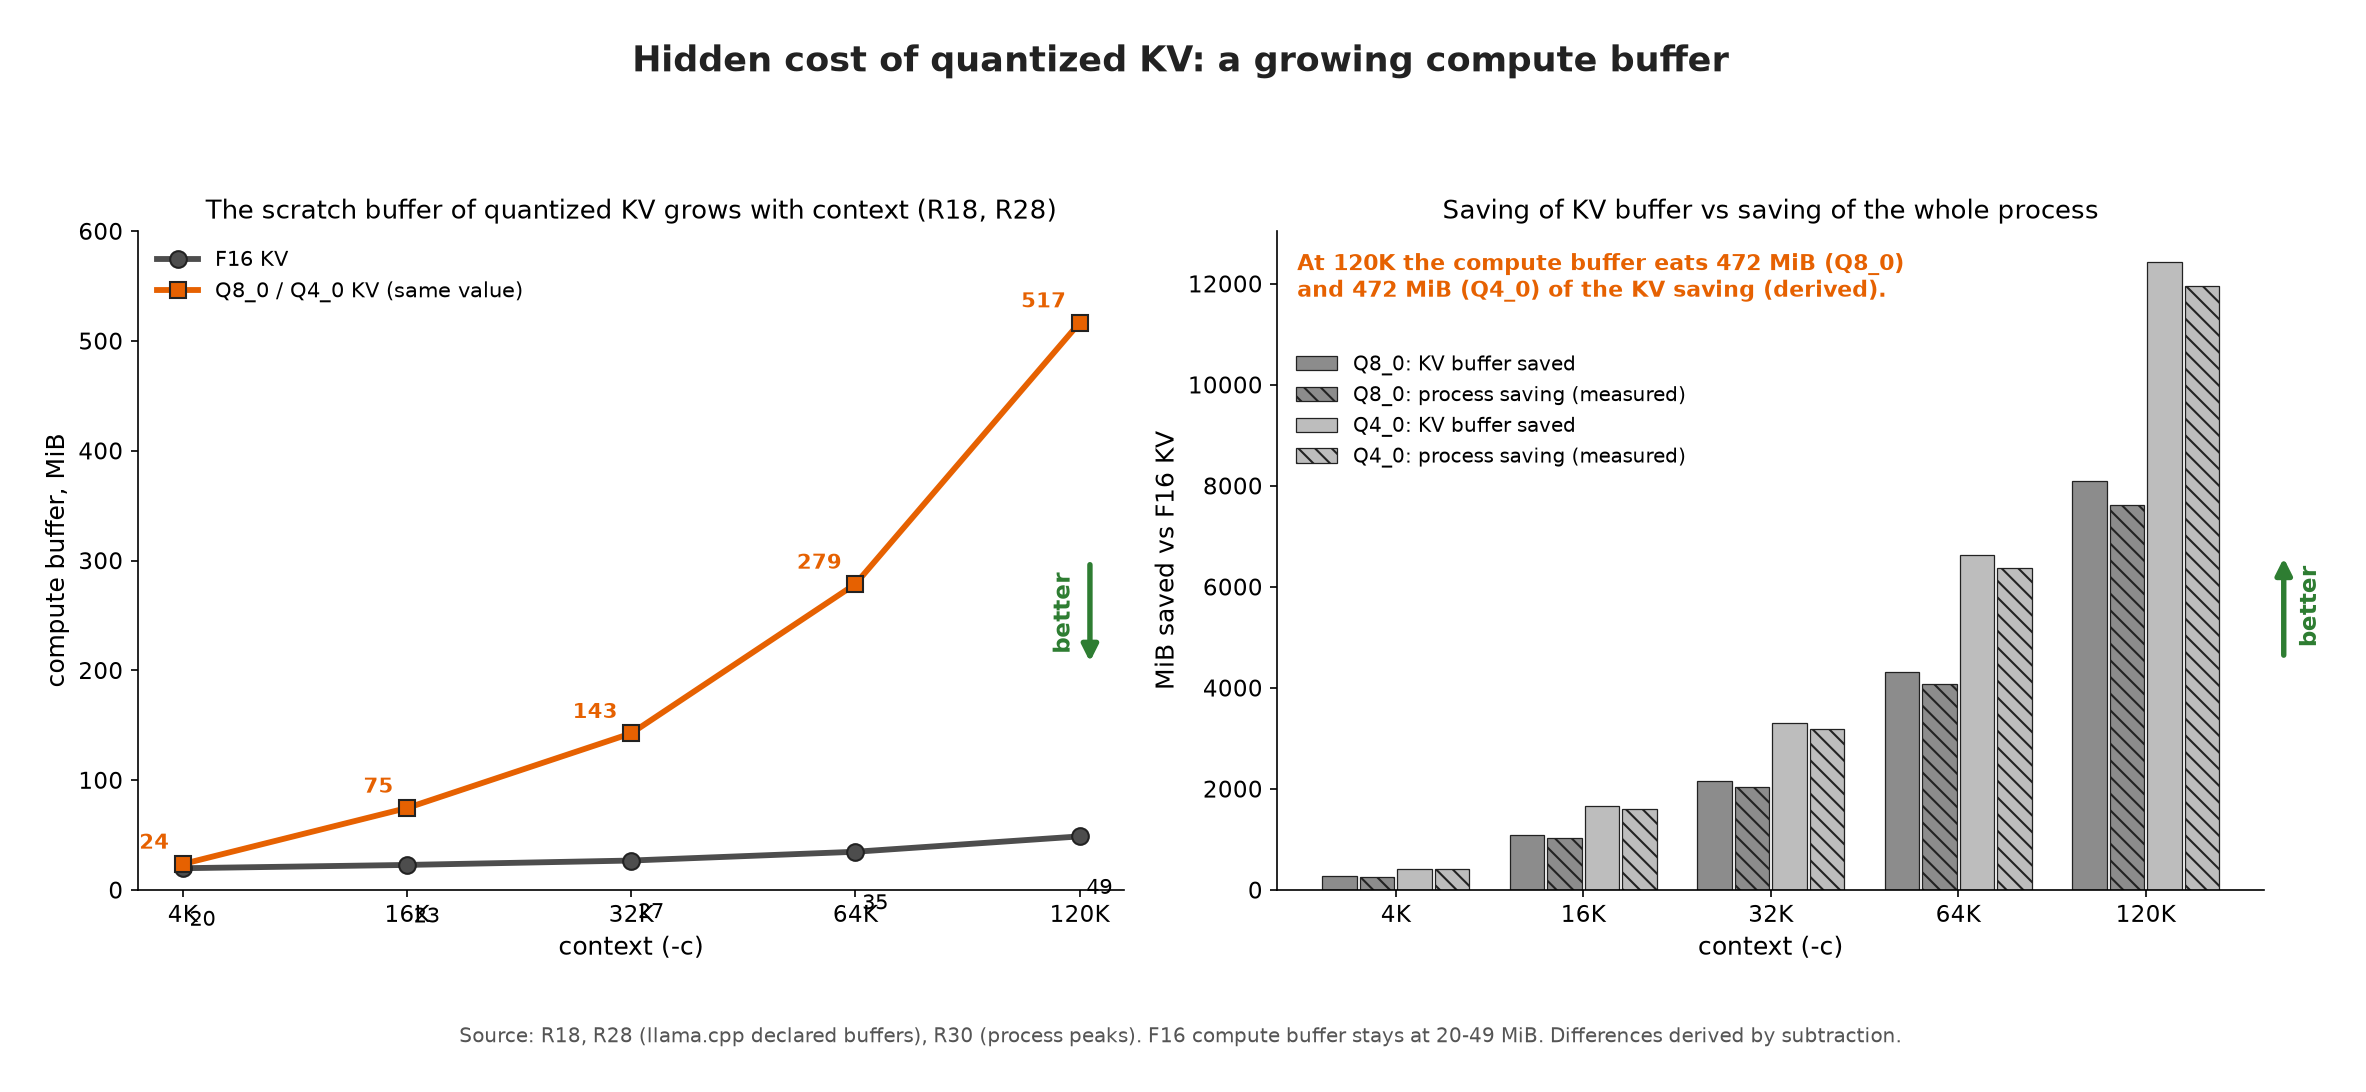
\includegraphics[width=\linewidth]{figures/fig35_compute_buffer_growth.png}\caption{The compute buffer of quantized KV grows from 24 to 517 MiB between 4K and 120K and eats 472 MiB of the KV saving at 120K (R18, R28, R30; difference derived). It is the f16 scratch of the quantized-KV FA path (\#24166).}\end{figure}

\begin{figure}[htbp]\centering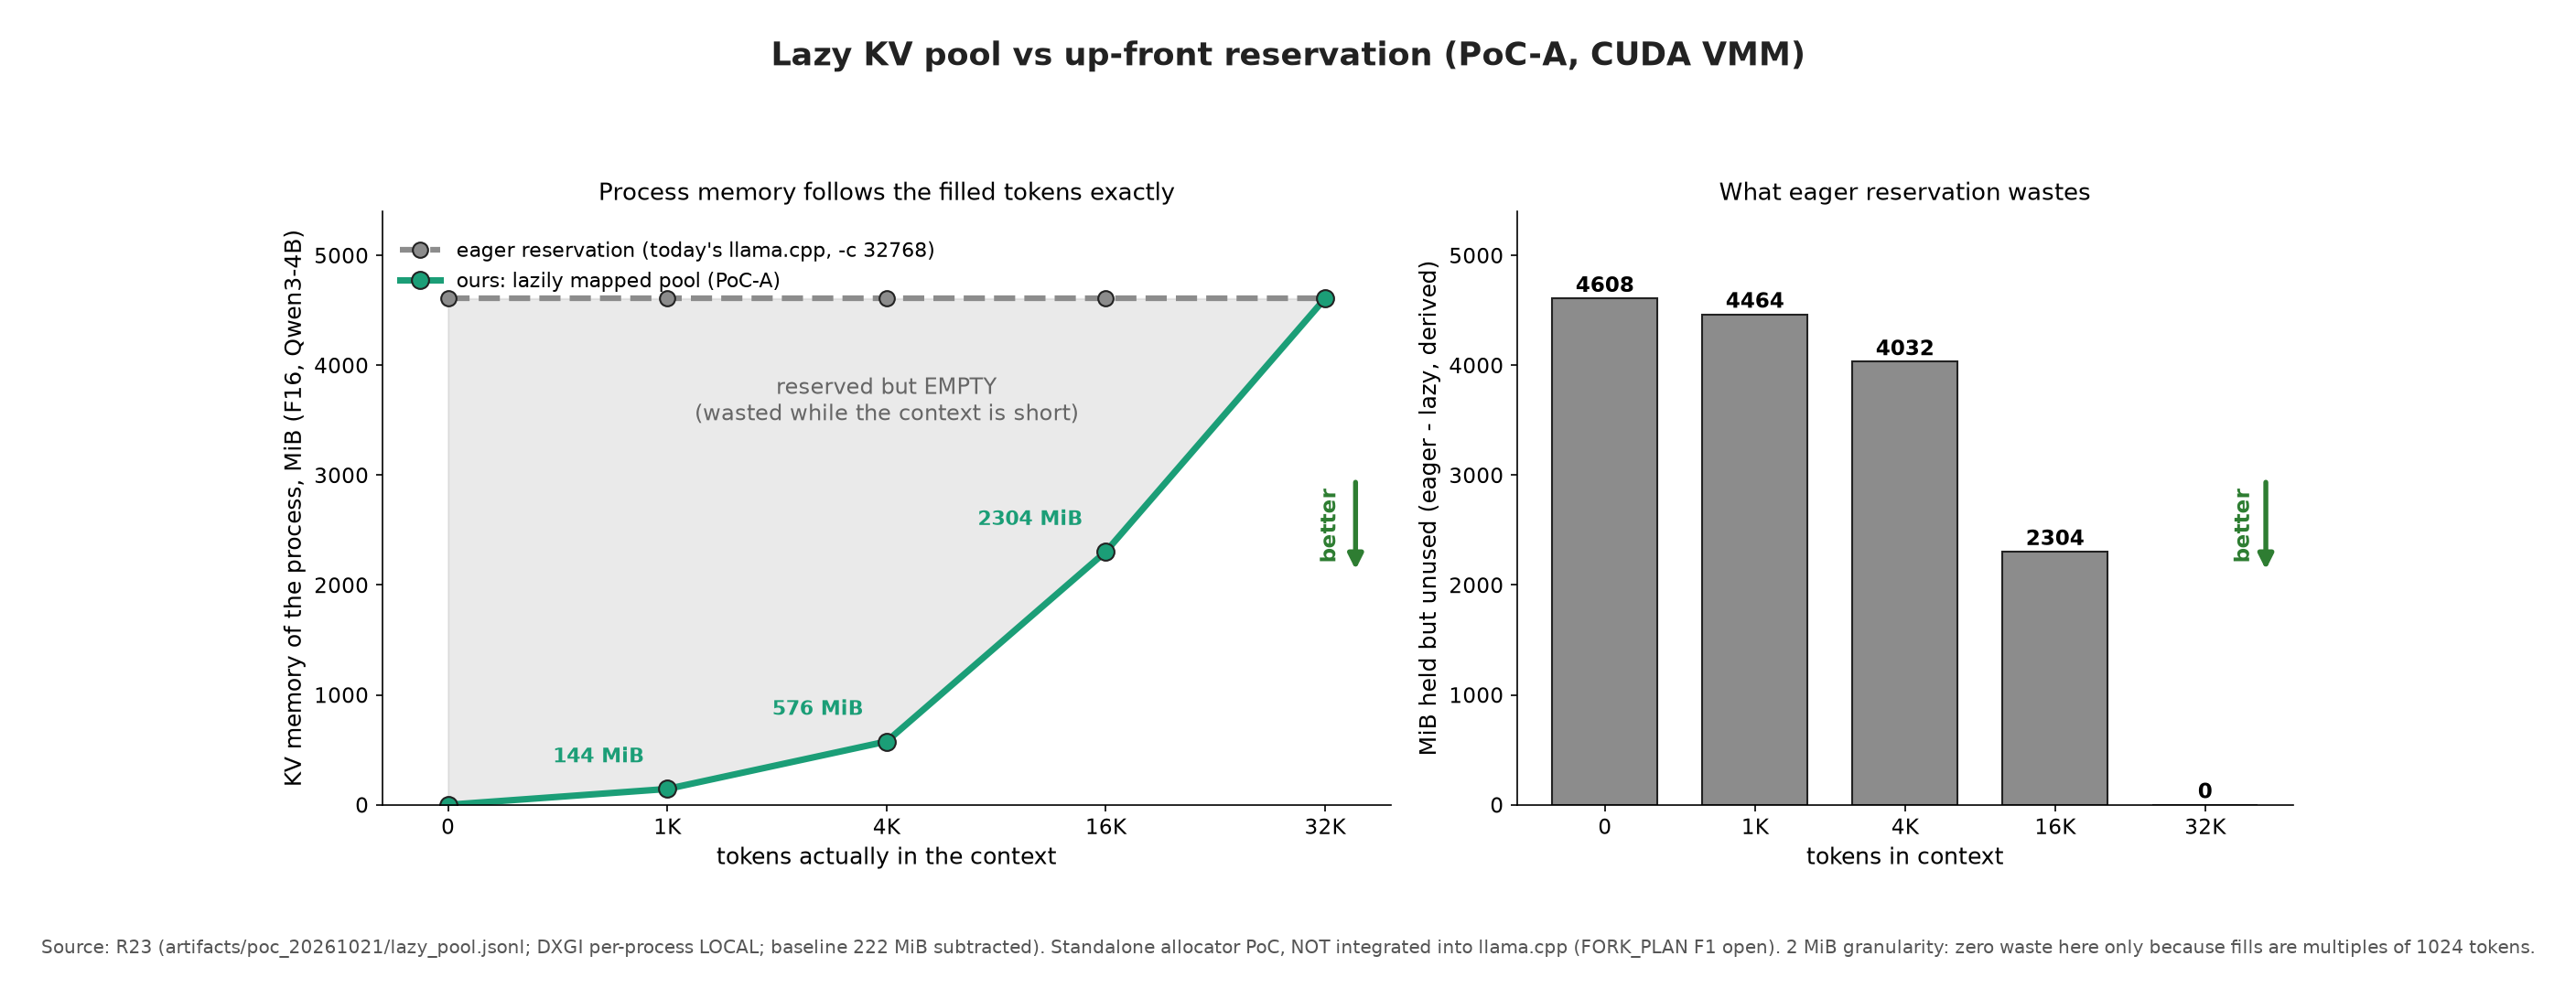
\includegraphics[width=\linewidth]{figures/fig21_lazy_pool_vs_eager.png}\caption{A lazily mapped KV pool (CUDA VMM) makes process memory follow the filled tokens: 144 MiB at 1K against 4,608 MiB reserved for -c 32768 (R23). This is a standalone allocator PoC reproducing a known technique (vAttention, kvcached), not something integrated into llama.cpp.}\end{figure}

\section{Further measurements}

\begin{itemize}
\item \textbf{E3, int4 granularity} (R40; same weights): code entropy is 0.80 bits for per-tensor int4, 2.88 for per-row, 3.60 for group-128 asymmetric (AWQ/GPTQ-like layout, without activation-aware scaling) and 3.59 for group-32. Only per-tensor int4 leaves large lossless headroom, which agrees with Tan et al. ("int4" 0.6--1.0 bits; group formats 1.1--1.3$\times$ above their bound) and with our 2--7\% for k-quants.
\item \textbf{E4, BF16 vs F16 KV (R41):} we captured the KV of the same prompts with \texttt{-ctk/-ctv bf16}. Exponent and sign entropies match F16 within 0.002 bits, as they should, since the activations are the same. The difference is the mantissa: 7 bits, of which the top 3 carry 2.95 bits and the low 4 are noise, against 10 bits in F16. The context estimate falls from 0.83/0.84 (F16, K/V) to 0.64/0.65 (BF16), and the TRACE-like codec from 0.84/0.86 to 0.655/0.677 (1.48--1.53$\times$). The dtype accounts for most of the distance to TRACE's 1.81--1.88$\times$ on BF16 KV of Llama-3.1-8B. The remainder (1.53$\times$ vs 1.8$\times$) depends on model or data and needs a capture from a model without QK-norm. In llama.cpp BF16 and F16 KV both take 16 bits, so BF16 KV only pays off together with a lossless codec. (Figure 14)
\end{itemize}


\begin{figure}[htbp]\centering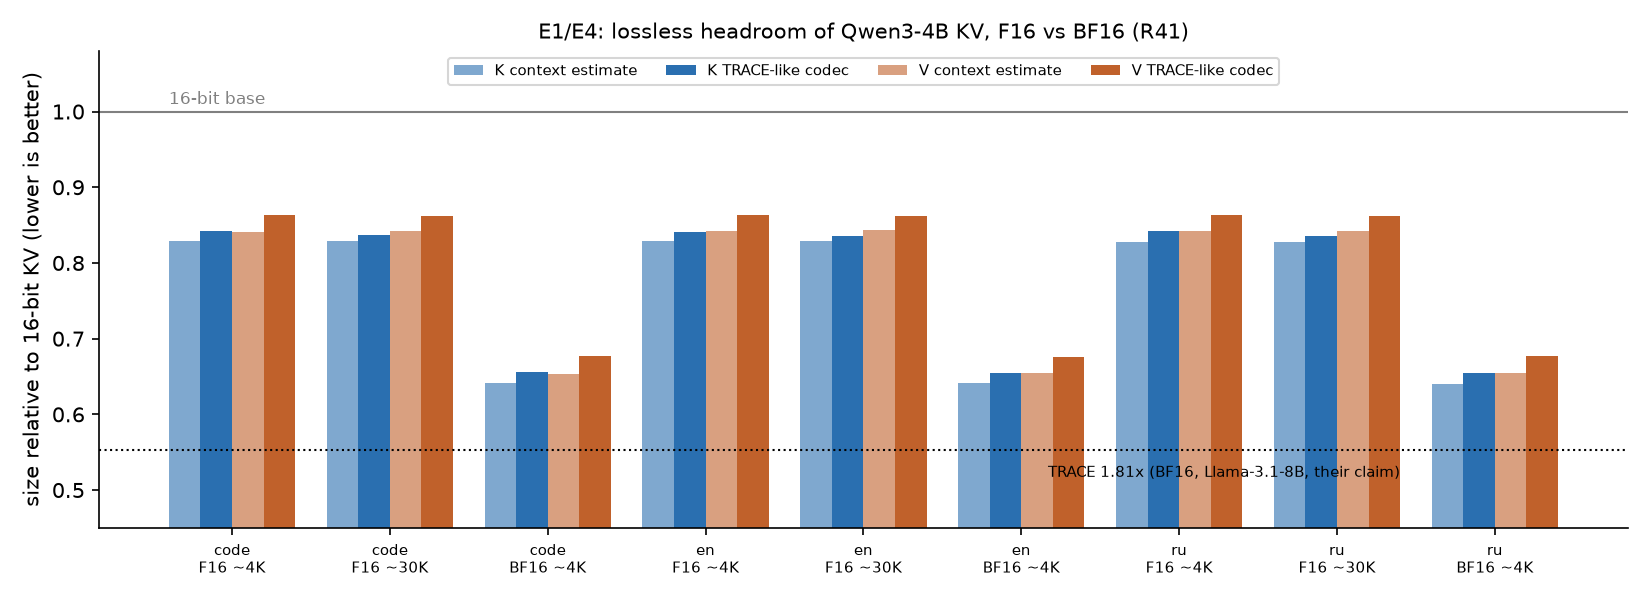
\includegraphics[width=\linewidth]{figures/fig51_e1_e4_lossless_kv.png}\caption{E1/E4: lossless size relative to 16-bit KV for three texts, two lengths and F16 vs BF16 KV of the same activations (context estimate and TRACE-like codec, K and V; R41). The dotted line is TRACE's reported 1.81$\times$ on BF16 KV of another model.}\end{figure}

\section{Inside llama.cpp: the combined fork (rows A--D)}

Sections 4--6 measure formats through CPU codecs, emulation and microbenchmarks. To see what they are worth in
practice we implemented the formats as real ggml types with CUDA kernels in a llama.cpp fork and measured them
under normal inference (R60--R87). Weight types: \texttt{CQ\_BF16W4} (BF16 with a 4-bit exponent offset per 64 values
plus an escape list; lossless, 12.1 bits), \texttt{CQ\_BF16H} (Huffman-coded exponent, as DFloat11; lossless, 11.1
bits) and \texttt{CQ\_BF16W3} (3-bit offset; lossy, 11.1 bits), each with a fused batch-1 GEMV that reproduces the
summation order of llama.cpp's BF16 kernel. KV types: \texttt{f16e3} (lossless: 3-bit exponent window, in-block
escapes, overflow pool), \texttt{f16d4} (F16 without its 4 low mantissa bits, 12 bits) and \texttt{q4o} (Q4\_0 plus the 2
largest of every 128 values in F16, 5.0 bits). One single-token FlashAttention kernel serves all query heads of
a GQA group from a single K/V read ("GQA kernel"); it also runs on unchanged F16, Q8\_0 and Q4\_0 caches. Both
branches were merged into one build (\texttt{cq/combined}), so rows A--D of every pair come from the same binary.
Patches: \texttt{artifacts/fork\_patches/} (\texttt{git format-patch} against the pinned commit \texttt{ed7ac35e}).

\textbf{Setup.} Pairs (weights, KV): (BF16, F16), (Q8\_0, Q8\_0), (Q4\_K\_M, Q4\_0) on Qwen3.5-2B, plus the KV types
alone on Qwen3-4B Q4\_K\_M. Row A is both bases, B our weights, C our KV (or our kernel on the base KV), D both.
llama-bench decode (tg64) and prefill (pp512) after 4K, 32K and 120K filled tokens, ABBA order, 12--18 samples
per cell; process VRAM from the fork's own DXGI report; quality as KL at context 4096 against row A and against
BF16 + F16 KV, plus the 39-case task suite; lossless rows checked by comparing raw float32 logits (R80). The
Q8\_0 and Q4\_K\_M bases have no lossless row: no GPU-decodable code saves more than 3.4\% there (R64), and every
fixed-rate KV variant was larger than its base (R33). We locked the GPU for every series, but desktop
applications still held it at 5--13\% utilisation at idle; noisy cells were re-measured (R86).

\textbf{Bit identity (R81).} W4 and H weights give logits identical to BF16, both as one prefill batch and token by
token, with and without kernel fusion. W4/H + f16e3 is identical to BF16 + f16e3. f16e3 KV is identical to F16
KV on Qwen3-4B (head size 128) when both use the same kernel path. On Qwen3.5-2B (head size 256) the stored
values are exact, but the decode kernel sums in a different order after 128 positions (logit differences
$\leq$ 1e-3, same greedy output). f16e3 stays lossless only while its overflow pool has room: the default 16 MiB
pool is a bump allocator and was full after about 8K tokens of real text on Qwen3-4B, after which some
superblocks lose values. That is a defect of the current implementation.

\textbf{Table 7.1.} Qwen3.5-2B, decode relative to row A (4K / 32K / 120K), process-VRAM change at 120K and KL vs A (context 4096). Row A in absolute terms: BF16 + F16 159 / 149 / 120 tok/s and 5,838 MiB; Q8\_0 + Q8\_0 236 / 207 / 145 tok/s and 3,466 MiB; Q4\_K\_M + Q4\_0 272 / 220 / 151 tok/s and 2,400 MiB (R82--R84, R86).

\begin{table}[h]\centering\scriptsize
\resizebox{\linewidth}{!}{%
\begin{tabular}{llllll}
\toprule
Pair & Row & Weights size & VRAM at 120K & Decode $\times$A & KL vs A \\
\midrule
BF16 + F16 & B lossless W4 & 0.759 & --846 MiB & 1.03 / 1.05 / 1.03 & 0 (bit-identical) \\
 & B lossless H & 0.696 & --1,074 MiB & 0.63 / 0.73 / 0.67 & 0 (bit-identical) \\
 & B lossy W3 & 0.695 & --1,074 MiB & 1.13 / 1.13 / 1.11 & 0.0008 \\
 & C lossless f16e3 & 1.000 & --50 MiB & 0.80 / 0.61 / 0.39 & 0 (prefill) \\
 & C lossy f16d4 & 1.000 & --360 MiB & 0.96 / 0.90 / 0.77 & 0.0002 \\
 & D lossless W4 + f16e3 & 0.759 & --896 MiB & 0.83 / 0.63 / 0.39 & 0 (prefill) \\
 & D lossy W3 + f16d4 & 0.695 & --1,434 MiB & 1.09 / 0.99 / 0.82 & 0.0010 \\
Q8\_0 + Q8\_0 & B lossy FFN $\rightarrow$ Q6\_K & 0.889 & --210 MiB & 1.04 / 1.04 / 1.02 & 0.0031 \\
 & C GQA kernel (same bytes) & 1.000 & 0 & 0.94 / 0.94 / 0.94 & 0 (prefill) \\
 & D & 0.889 & --210 MiB & 0.99 / 0.97 / 0.96 & 0.0031 \\
Q4\_K\_M + Q4\_0 & B lossy emb/output $\rightarrow$ Q4\_K & 0.899 & --126 MiB & 1.03 / 1.08 / 1.01 & 0.029 \\
 & C lossy q4o & 1.000 & +44 MiB & 0.84 / 0.70 / 0.52 & 0.020 \\
 & C GQA kernel (same bytes) & 1.000 & 0 & 0.97 / 1.00 / 1.04 & 0 (prefill) \\
 & D emb $\rightarrow$ Q4\_K + GQA kernel & 0.899 & --126 MiB & 1.00 / 1.05 / 1.07 & 0.029 \\
\bottomrule
\end{tabular}}
\end{table}

Only 6 of 24 layers in Qwen3.5-2B keep a KV cache, so KV formats move process memory by a few hundred MiB at
most, and our GQA kernel loses to the stock path at its head size 256 with 2 KV heads: on plain F16 data
0.97 / 0.87 / 0.75$\times$ of the stock F16 path (R86). f16d4 through the same kernel is 0--3\% faster than F16 through
it, so the loss belongs to the kernel, not the format. Task scores stay within $\pm$1 of row A (26--28 of 39) in
every row; the lossless rows answer 39 of 39 cases identically to A (R82--R84).

\textbf{Table 7.2.} Qwen3-4B Q4\_K\_M (KV in all 36 layers, head size 128, 8 KV heads), 120K filled tokens (R85). Quality of these KV types on this model: R45 (KL vs F16 KV at 4K).

\begin{table}[h]\centering\scriptsize
\resizebox{\linewidth}{!}{%
\begin{tabular}{lllll}
\toprule
KV & Process VRAM & Decode tok/s & vs F16 & KL vs F16 KV \\
\midrule
F16 & 20,290 MiB & 37.6 & 1.00 & --- \\
f16d4 (ours, 12 bit) & 16,288 MiB & 43.4 & 1.15 & 0.0028 \\
Q8\_0, stock kernel & 12,486 MiB & 24.2 & 0.64 & 0.0035 \\
Q8\_0, our GQA kernel & 12,486 MiB & 41.6 & 1.11 & as stock \\
Q4\_0, stock kernel & 8,148 MiB & 22.6 & 0.60 & 0.068 \\
Q4\_0, our GQA kernel & 8,148 MiB & 43.7 & 1.16 & as stock \\
q4o (ours, 5 bit) & 8,698 MiB & 23.7 & 0.63 & 0.033 \\
f16e3 (ours, lossless) & 19,832 MiB & 5.1 & 0.14 & 0 while the pool has room \\
\bottomrule
\end{tabular}}
\end{table}

At 32K the GQA kernel reaches 1.43$\times$ (Q8\_0) and 1.53$\times$ (Q4\_0) of the stock path, at 4K 1.05$\times$ and 1.07$\times$; prefill
is unchanged.

\textbf{Practical value.} (1) Lossless weight compression inside the engine is usable: W4 makes a BF16 model 24\%
smaller with identical outputs and slightly faster decode (1.03--1.05$\times$); prefill costs 8--16\%. (2) The biggest
speed gain comes not from fewer bytes but from reading each K/V row once per GQA group: on a full-KV model this
turns quantized KV from 36--40\% slower than F16 into 11--16\% faster at 120K, with 38--60\% less memory. Upstream
PR \#30202 reaches 0.86 of F16 for Q8\_0 on the same GPU (R39). (3) A 12-bit KV type with F16-class quality
(f16d4) saves 20\% of process memory at 120K and decodes 15\% faster than F16 on Qwen3-4B. (4) Lossless KV
compression did not pay off: f16e3 saves less than 5\% of KV bytes and its decoder makes decode 1.2--7$\times$ slower.
(5) We built no fast lossy type below the Q8\_0/Q4\_0 KV bases; q4o buys quality (half the KL of Q4\_0) for 11\%
more bytes. All KV speed results depend on the attention shape of the model: the same kernel is slower on
Qwen3.5-2B.

\begin{figure}[htbp]\centering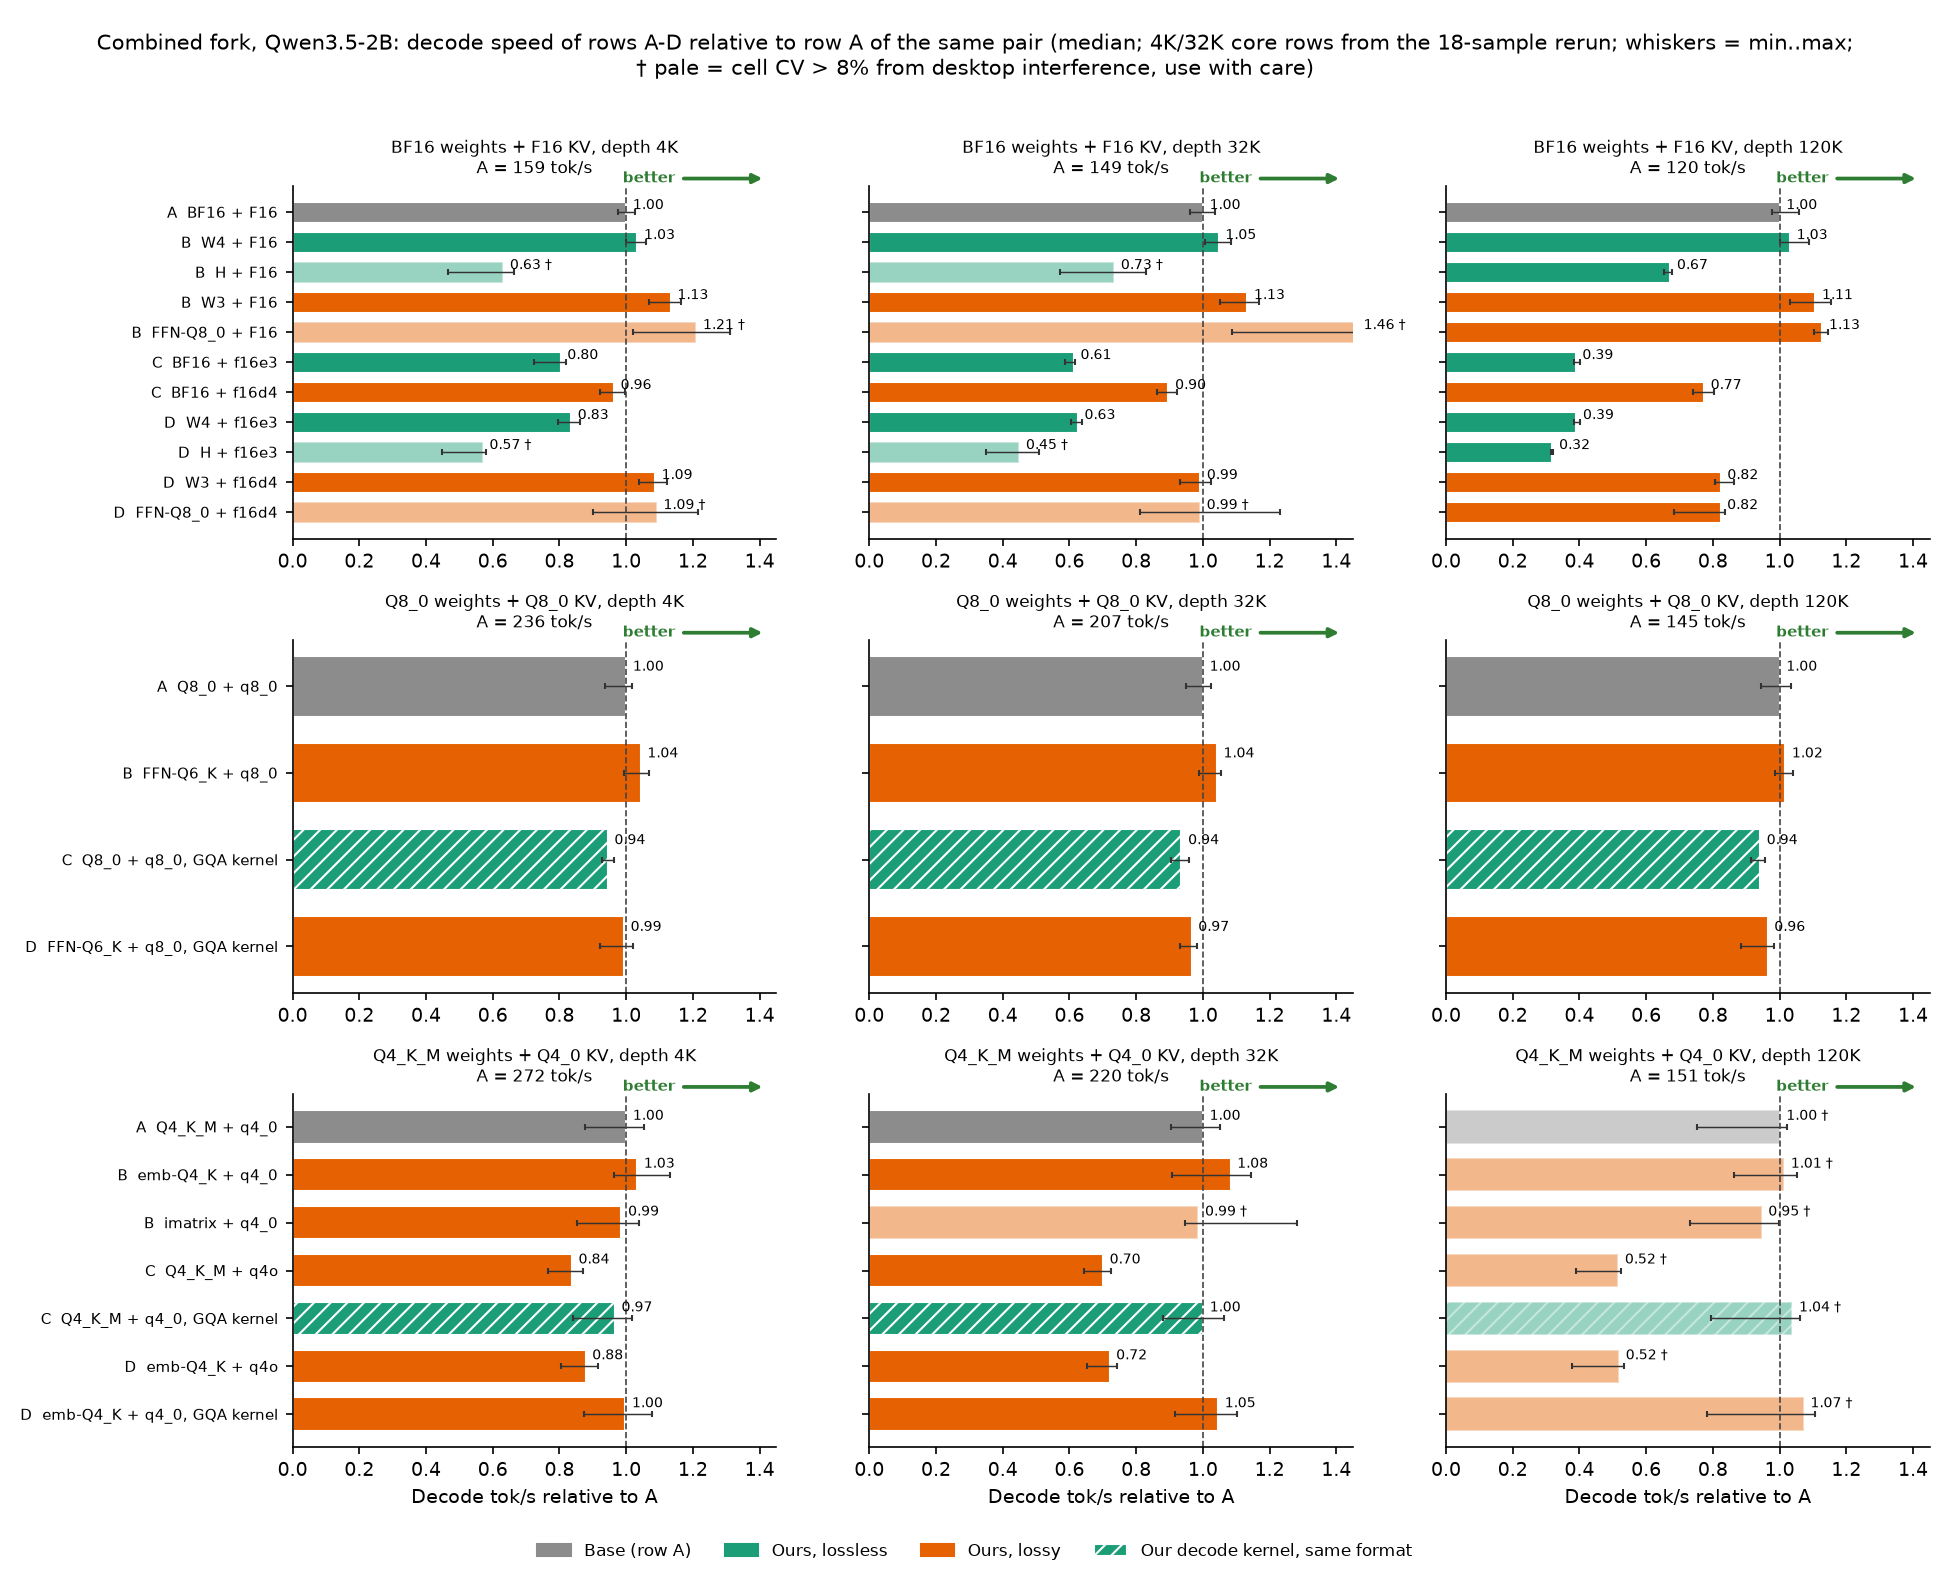
\includegraphics[width=\linewidth]{figures/fig80_combo_decode_ad.png}\caption{Combined fork, Qwen3.5-2B: decode speed of rows A--D relative to row A, per pair and depth (R82--R86). Grey = base, green = ours lossless, orange = ours lossy, hatched = our decode kernel on an unchanged format; pale bars marked † are cells with CV > 8\% caused by desktop interference.}\end{figure}

\begin{figure}[htbp]\centering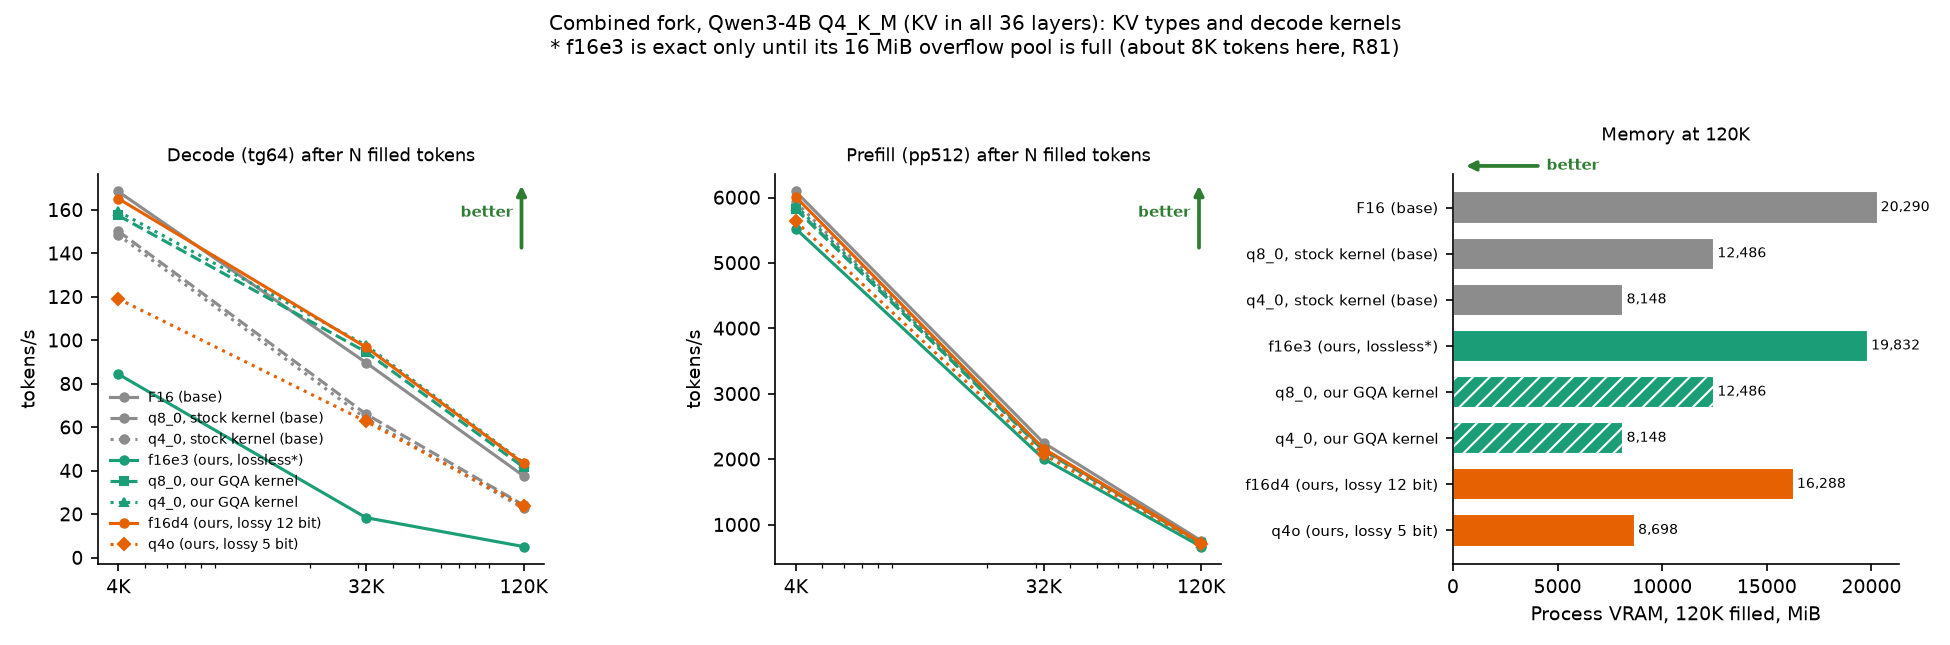
\includegraphics[width=\linewidth]{figures/fig84_combo_qwen3_4b_kv.png}\caption{Qwen3-4B Q4\_K\_M in the combined fork: decode and prefill against filled depth for each KV type and kernel, and process memory at 120K (R85).}\end{figure}

\begin{figure}[htbp]\centering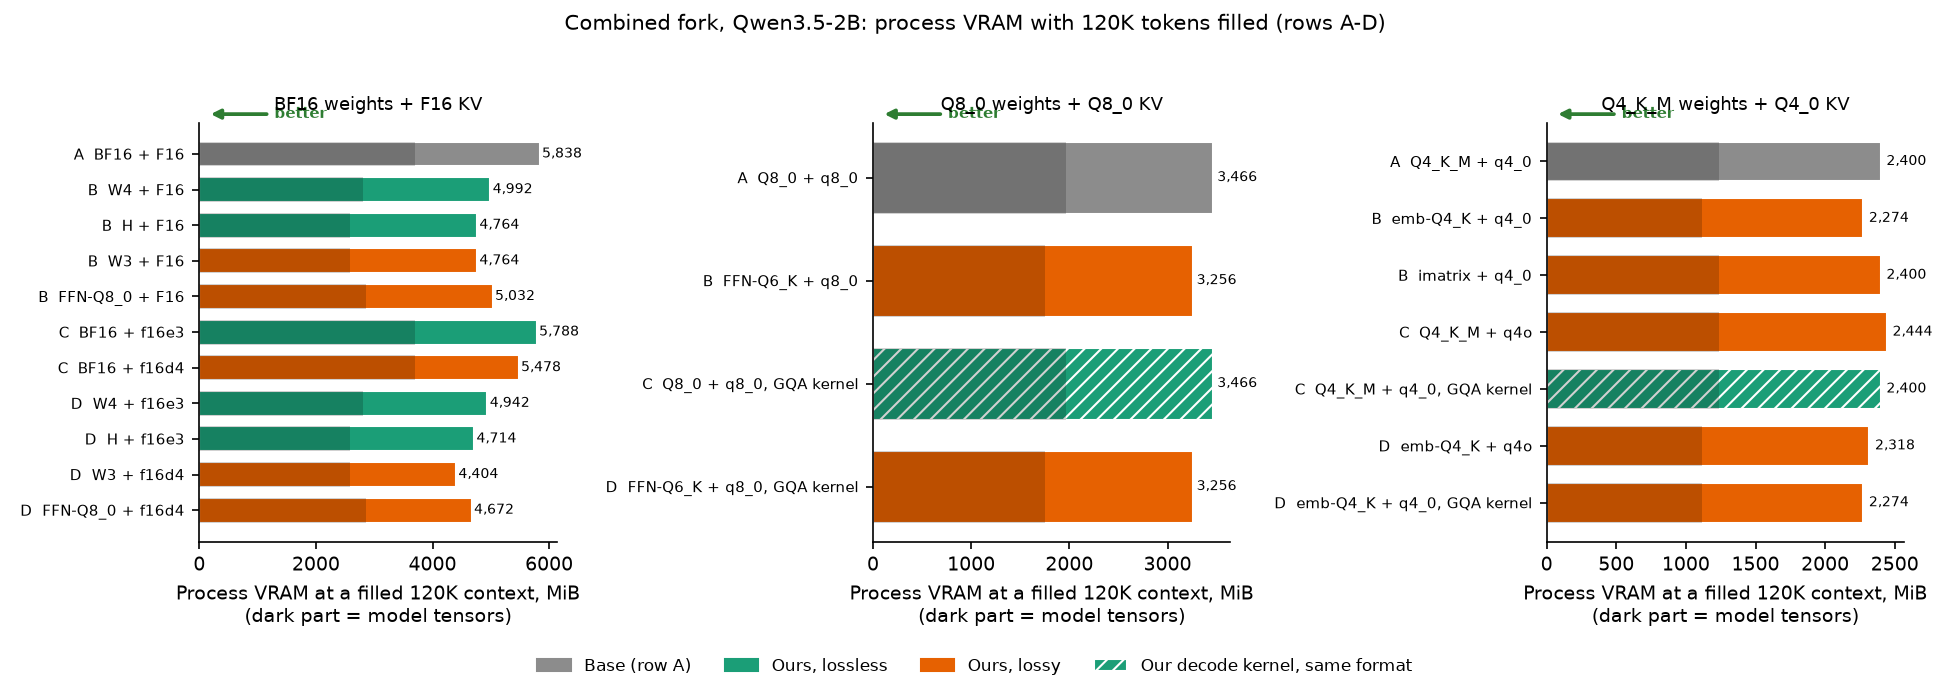
\includegraphics[width=\linewidth]{figures/fig82_combo_vram_120k.png}\caption{Process VRAM at a filled 120K context for rows A--D of each pair; the dark part is the model tensors (R82--R84).}\end{figure}

\begin{figure}[htbp]\centering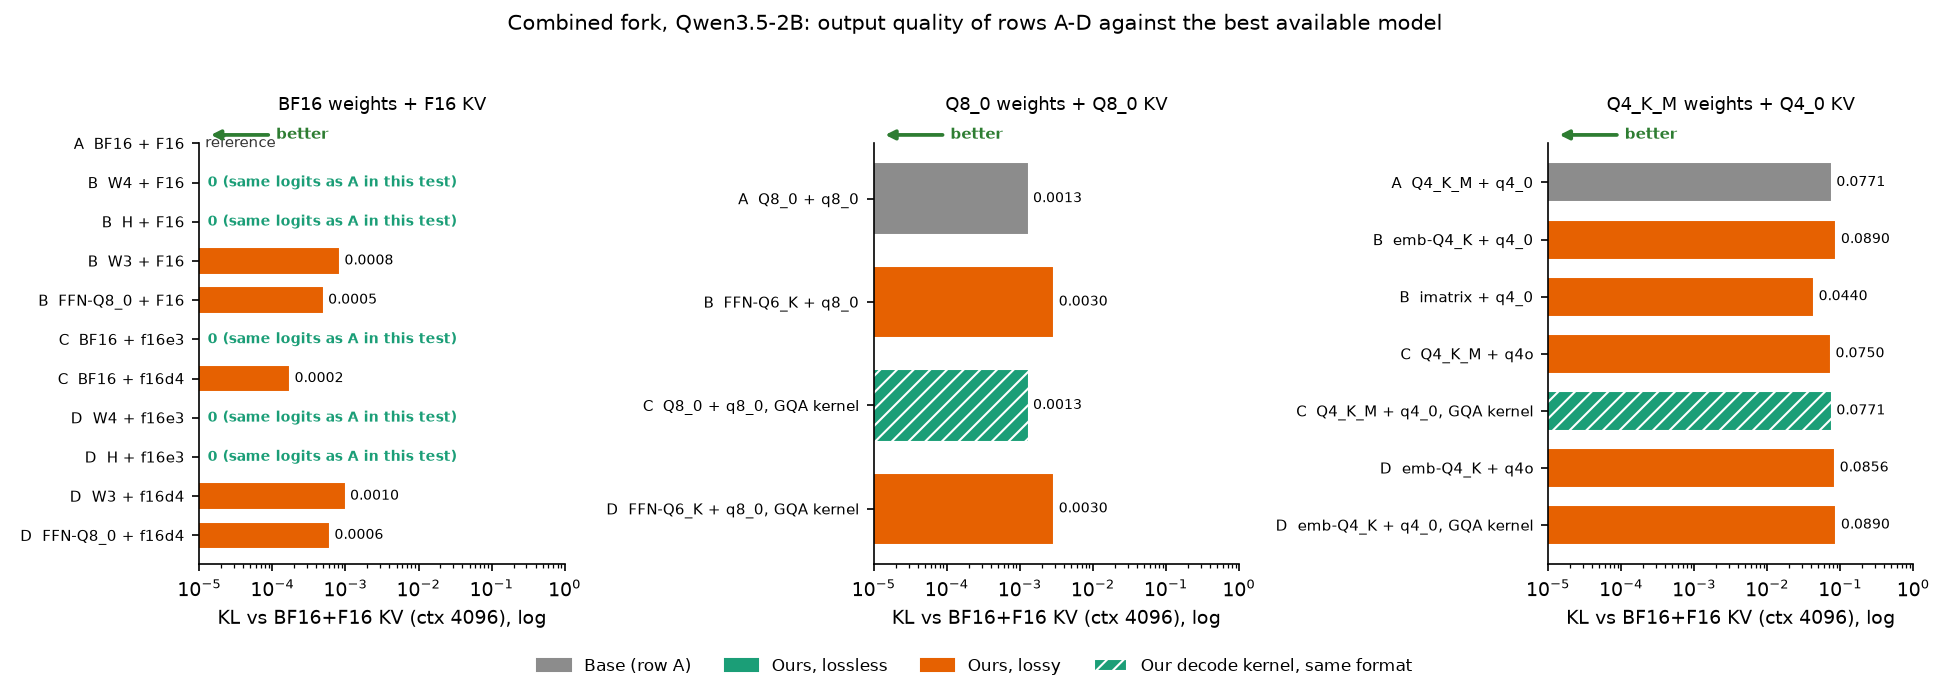
\includegraphics[width=\linewidth]{figures/fig83_combo_quality_kl.png}\caption{KL of rows A--D against BF16 weights + F16 KV at context 4096 (prefill path); 0 means identical logits (R82--R84).}\end{figure}

\begin{figure}[htbp]\centering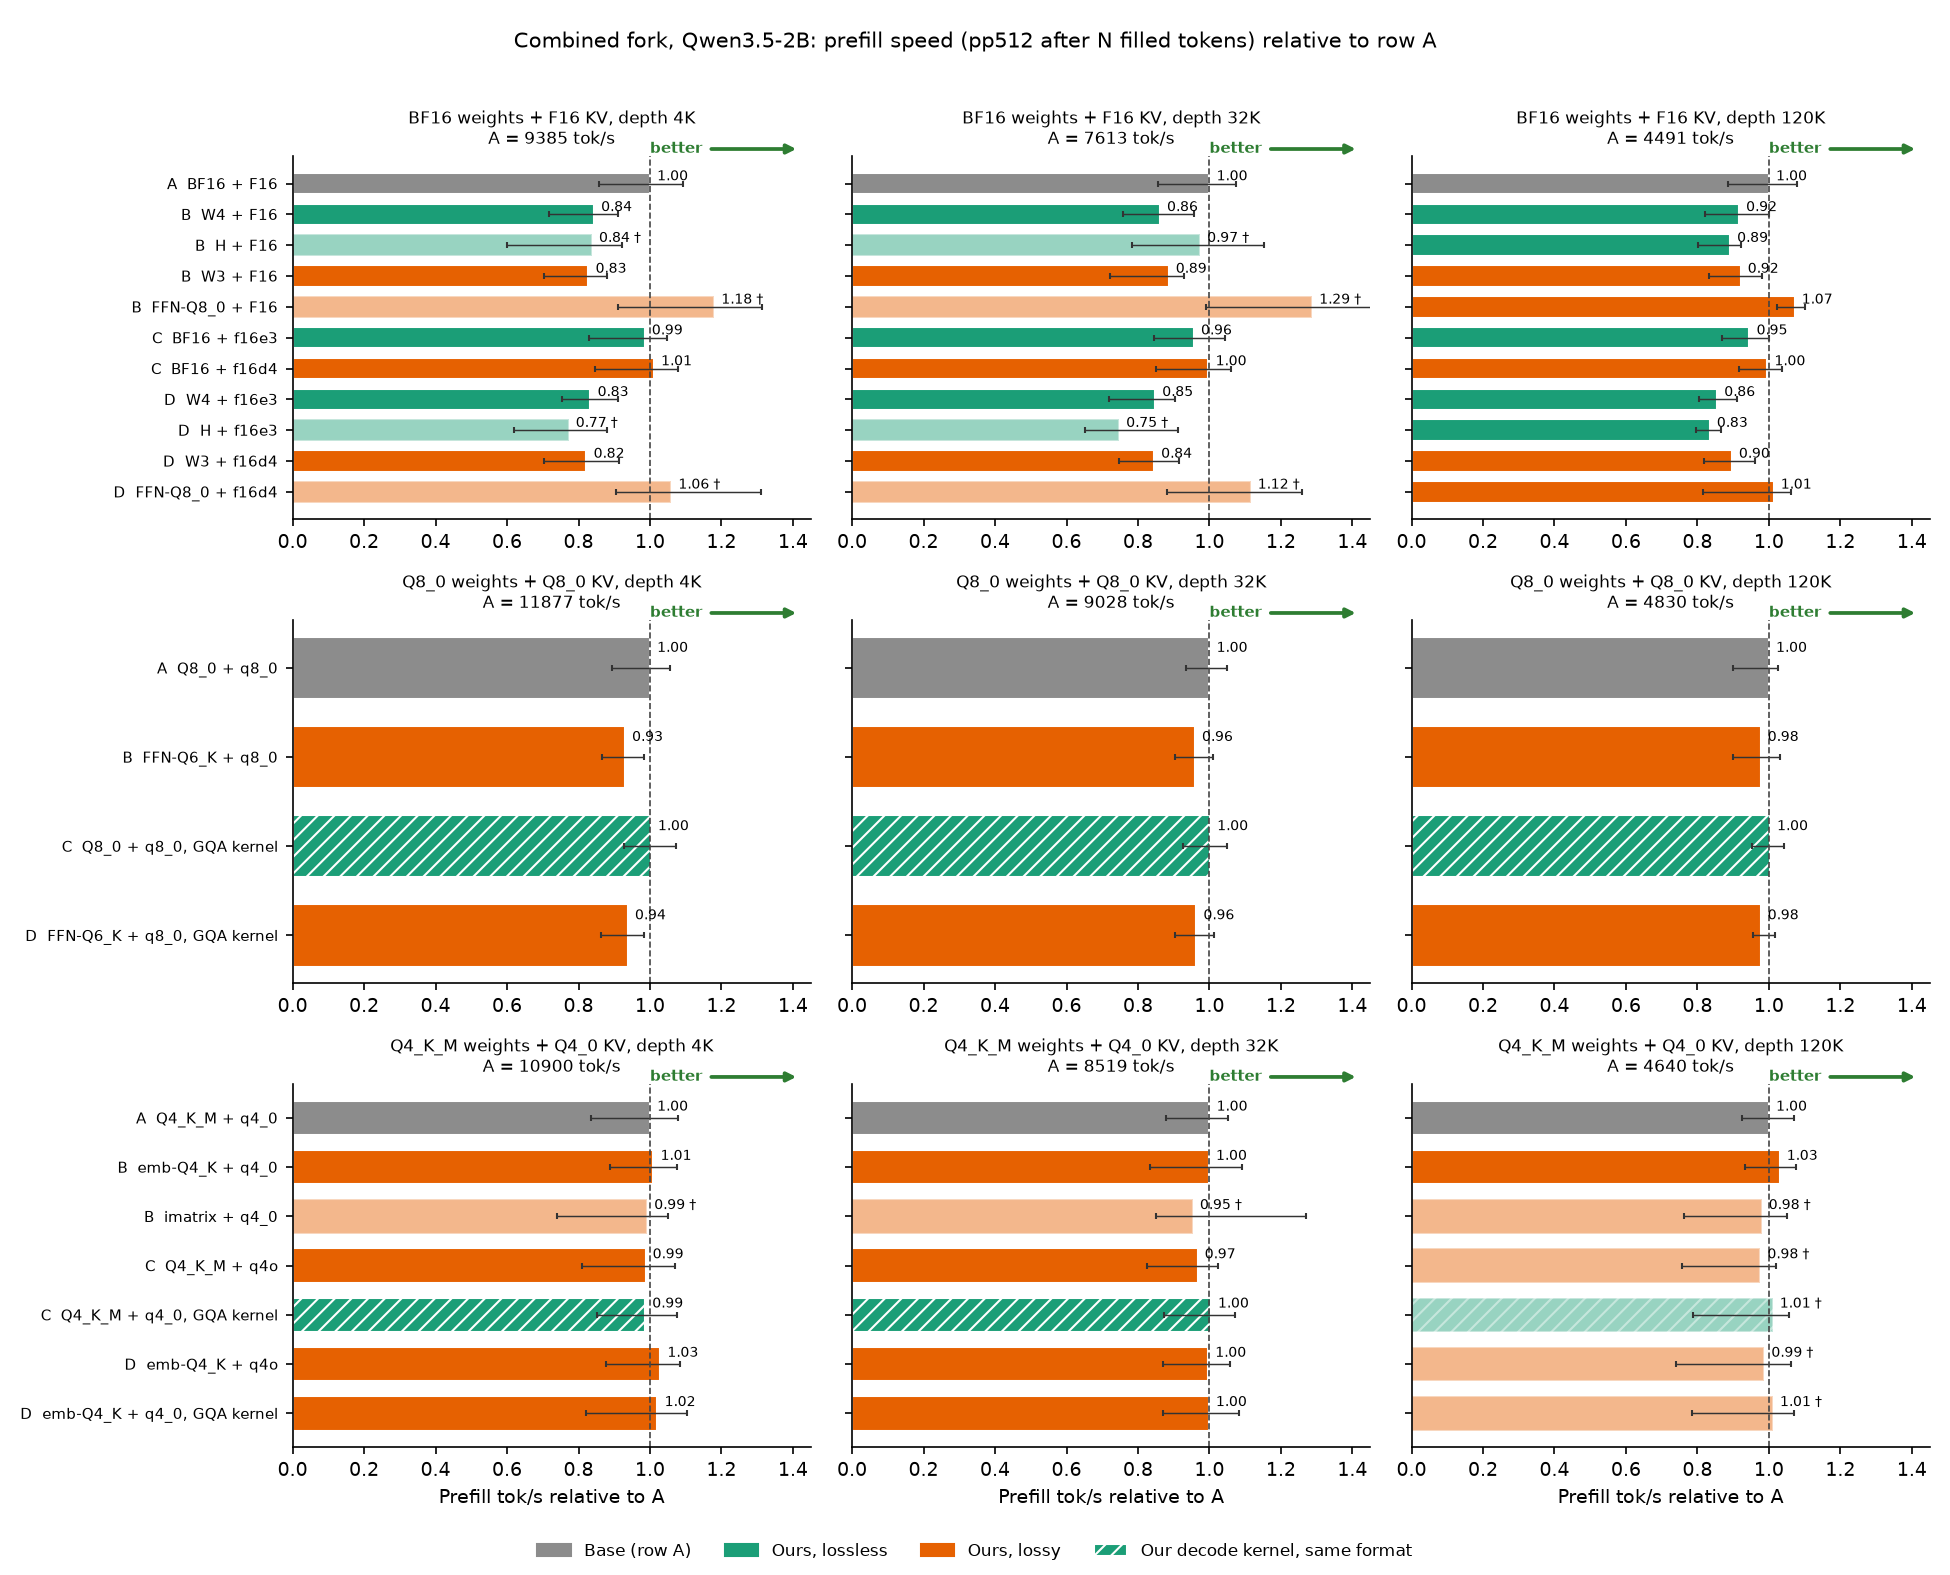
\includegraphics[width=\linewidth]{figures/fig81_combo_prefill_ad.png}\caption{Prefill speed of rows A--D relative to row A (R82--R86). Our weight types decode every weight into a BF16 scratch before the GEMM and lose 8--17\%.}\end{figure}
\section{Limitations}

KV work covers one model family (Qwen3 with QK-norm). No model without QK-norm is available locally, so the
part of the gap to TRACE's BF16 result on Llama-3.1-8B that the dtype does not explain (1.53$\times$ vs 1.8$\times$) stays
open. KV statistics come from Qwen3-4B captures. Three texts (code, English, Russian) and two lengths (about 4K
and 30K tokens) shift the lossless estimate by less than one point (R41), but other models and much longer
contexts may behave differently. The analysis covers every 6th layer. Emulation measures quality, not the speed
or memory of a packed format. Speed series before R37 ran on a shared GPU. E2 was measured on one GPU and one
model; the PRs were unmerged at the time of measurement and may change. We have no server-GPU measurements
(Appendix A is analytic). The task suite has 39 cases. Fork measurements (Section 7) rest on two models with very
different attention (Qwen3.5-2B: KV in 6 of 24 layers, head size 256, 2 KV heads; Qwen3-4B: all 36 layers, head
size 128, 8 KV heads), and the GQA kernel helps only the second; other shapes were not tested. Rows D with
lossless weights exist only for Qwen3.5-2B, because the weight types need a BF16 source and Qwen3-4B is
available only as Q4\_K\_M. KL in Section 7 is measured on the prefill path at context 4096; decode-path quality
rests on the 39 tasks, on raw-logit comparisons and on R43--R45. llama-bench fills the cache with random token
ids. Desktop applications kept the GPU busy at 5--13\% throughout the fork series; noisy cells were re-measured
(R86). The lossless KV type is exact only while its overflow pool has room (R81).

\section{Conclusion}

On a 24 GB consumer GPU with llama.cpp:
\begin{itemize}
\item KV: there is little room for lossless compression on top of F16 (about 16\%). Quantized KV offers more (7--21\%), but only with variable-rate coders. The GPU-addressable fixed-rate variants we built do not pay off in a non-fused kernel.
\item Lossy KV: a few extra bits on top of a base cost little quality. 12-bit KV is as good as Q8\_0, and keeping the 2 largest of every 128 values exact halves the KL of 4-bit KV (0.033 vs 0.068) for 11\% more bytes (R45).
\item Weights: the practical win is mixed-precision recipes with fast kernels (+16--18\% decode at --23\% size). Inside llama.cpp a lossless fixed-rate BF16 weight type is practical too: --24\% size, bit-identical outputs, 1.03--1.05$\times$ decode, 8--16\% slower prefill (R81--R86). A Huffman-coded type saves 30\% but decodes at 0.63--0.73$\times$.
\item BF16 KV leaves twice the lossless headroom of F16 KV on the same activations (0.65 vs 0.84 with the same codec): the 16-bit dtype, not the codec, sets most of that headroom.
\item What we can use today is capacity (--28\ldots{}--60\% KV memory, F16 at 120K fits). Speed gains depend on kernels, not on byte counts: upstream PR \#30202 alone lifts q8\_0 KV decode from 0.64 to 0.86 of F16 at 120K on this GPU, more than any byte reduction we could add on top. Our GQA-grouped decode kernel goes further on Qwen3-4B: Q8\_0 / Q4\_0 KV decode at 1.11 / 1.16$\times$ of F16 at 120K with 38 / 60\% less memory (R85); on Qwen3.5-2B (head size 256, 2 KV heads) the same kernel is slower than the stock path.
\item Lossless KV compression did not become practical: our lossless KV type saves under 5\% of KV bytes, decodes 1.2--7$\times$ slower and needs a reclaimable overflow store to stay exact (R81, R85).
\end{itemize}


\begin{figure}[htbp]\centering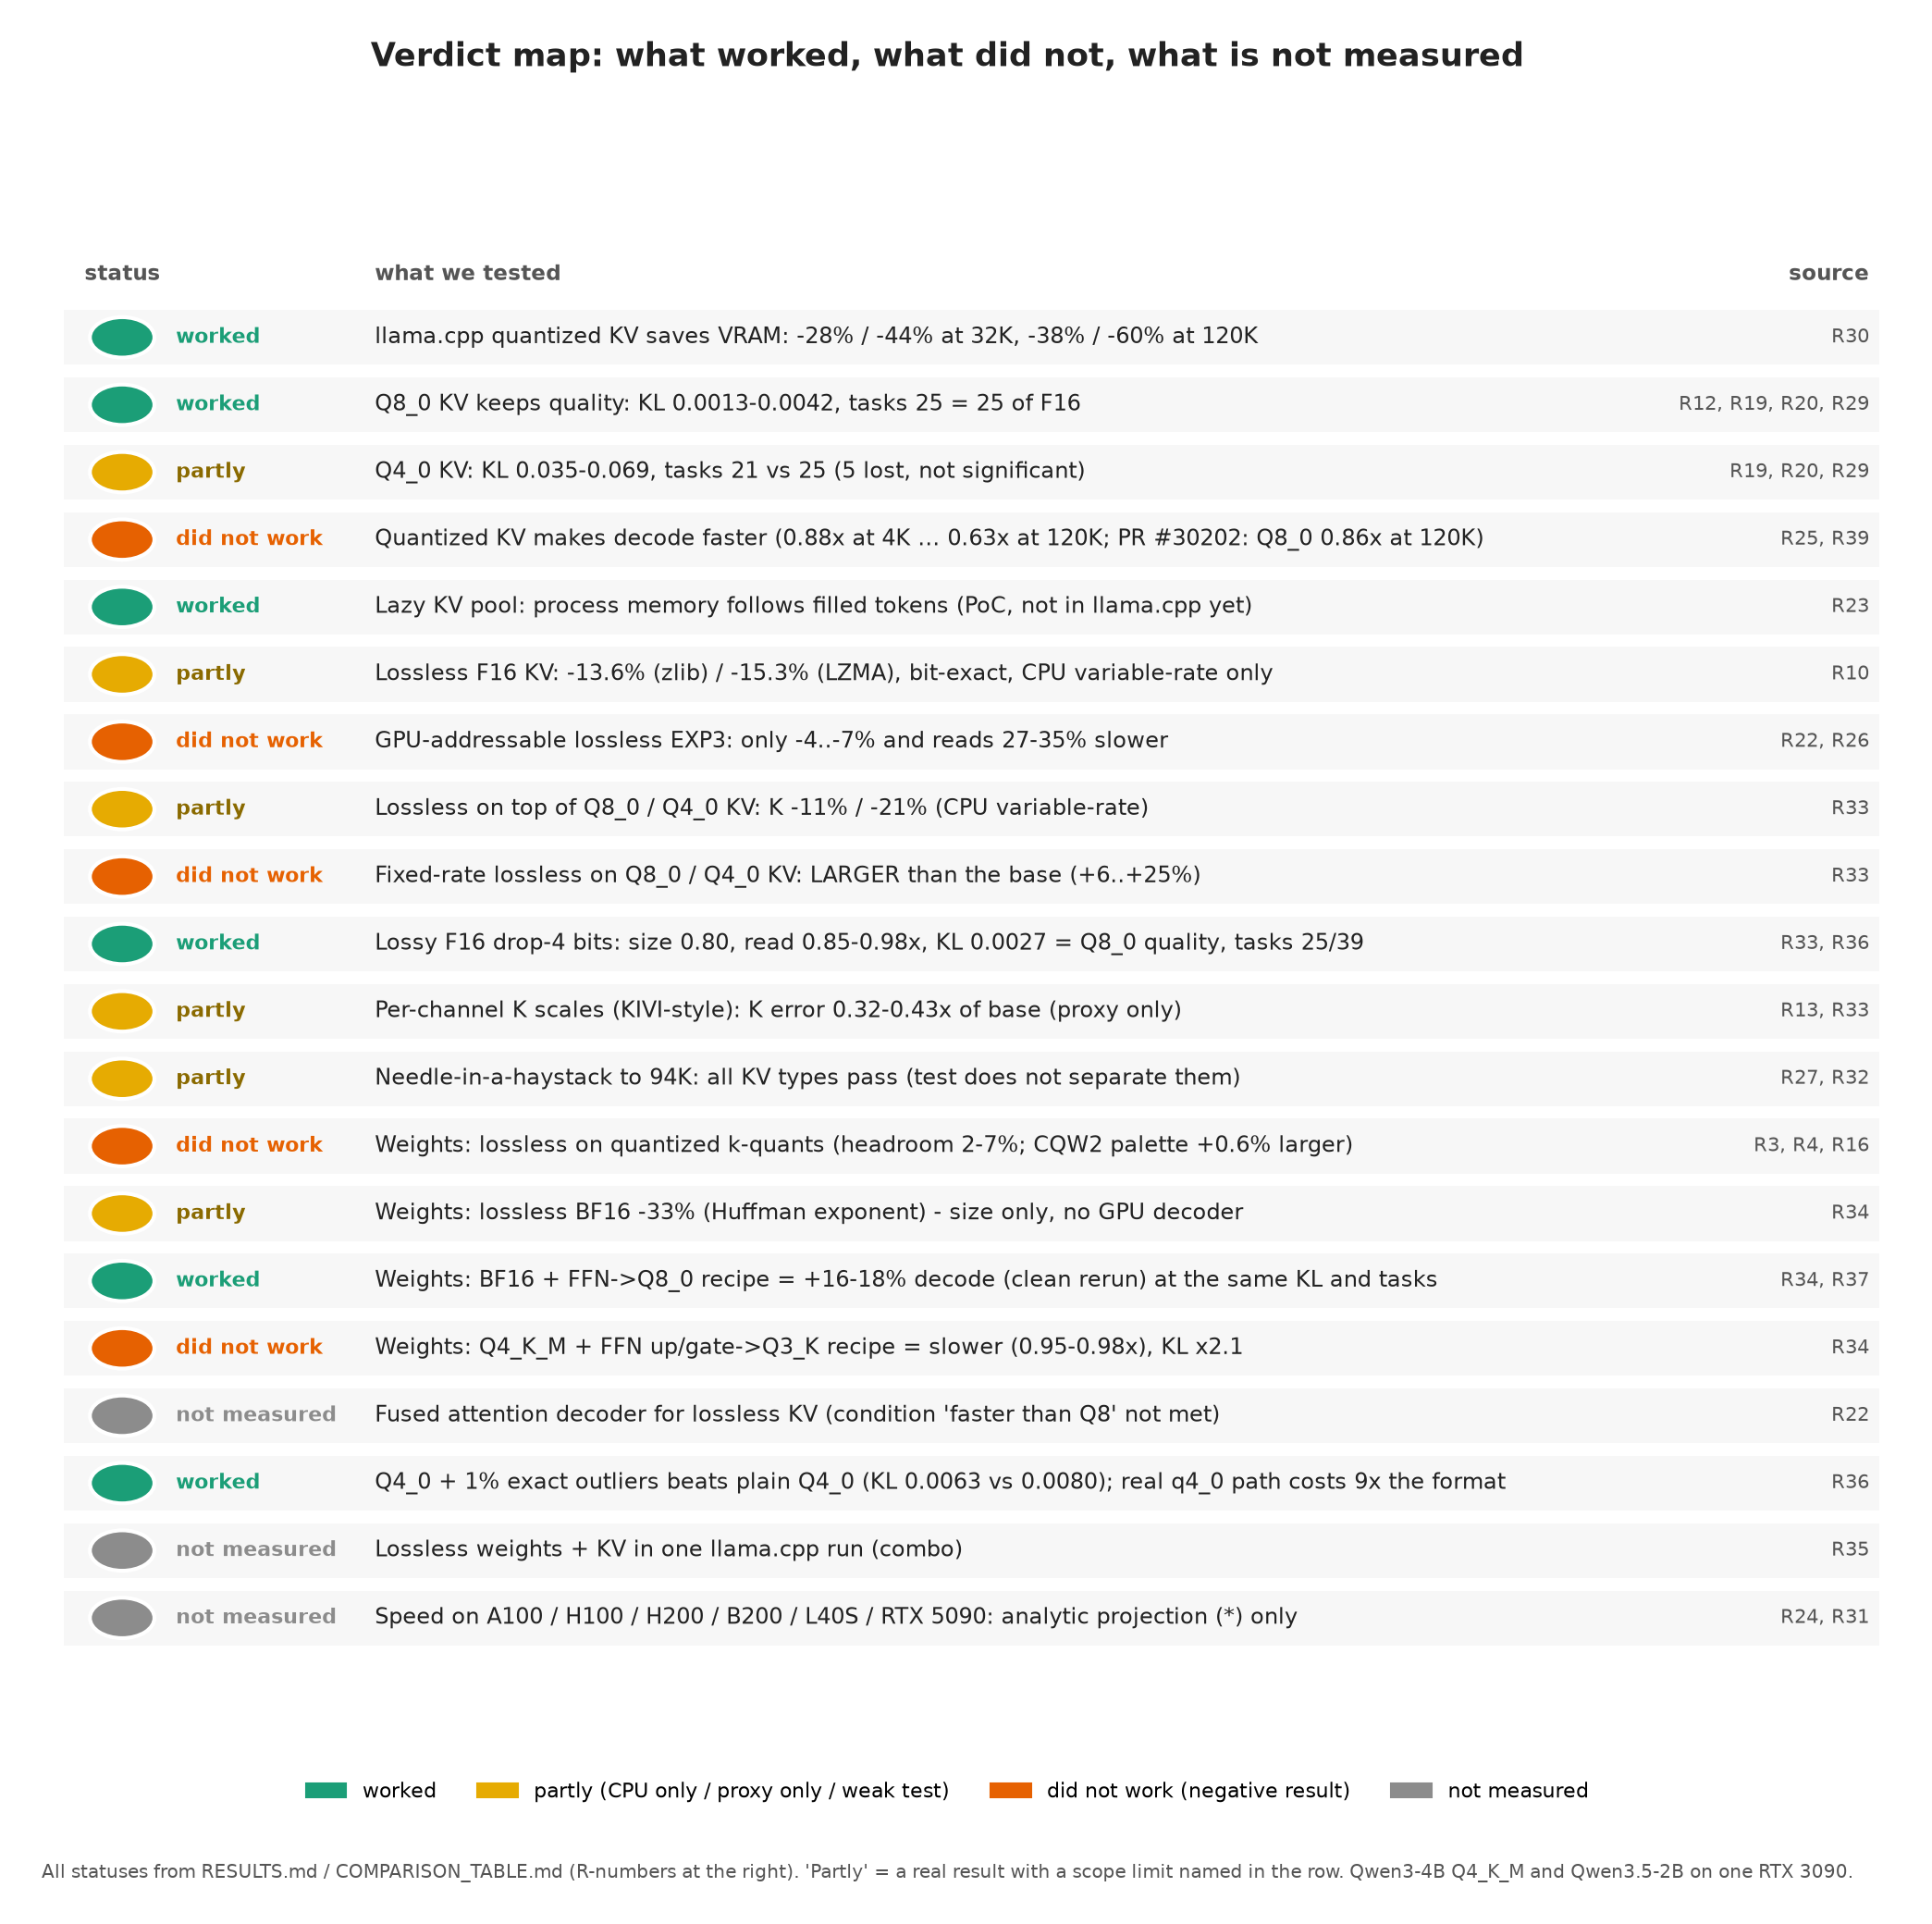
\includegraphics[width=\linewidth]{figures/fig29_verdict_map.png}\caption{Verdict map: what worked, what partly worked (CPU only, proxy only or weak test), what did not work, and what we never measured, with the RESULTS table for each row.}\end{figure}

\appendix
\section{Analytic model and projections (*)}

See PAPER\_V1\_EN.md \S{}1 and \S{}8, R15, R24, R31. None of it is validated, and none of it applies to tensor-core or
fixed-function decoders (BitDecoding, ZipServ).

* analytic projection, to be validated on this hardware. The speed projections assume scalar, llama.cpp-style decode kernels calibrated on the RTX 3090; they say nothing about FP8/INT4 tensor-core kernels of server stacks (vLLM, TensorRT-LLM, SGLang), so they must not be read as "compression loses on servers". Capacity gains are listed separately and do not depend on kernel speed.

\textbf{Method.} Decode time per token = weight bytes / bandwidth + KV bytes / (bandwidth $\times$ achieved efficiency) +
decode excess $\times$ elements read. The efficiencies and the scalar decode excess are calibrated on the RTX 3090
(R24, R31) and scaled to other cards by memory bandwidth and scalar FP32 throughput. For our lossless EXP3 the
excess is 2.01 ps per element (PoC-B, R26). \textbf{Ours lossy drop-4 (*)} uses the same model with a decode excess
of 1.08 ps per element, derived from the PoC-C microbenchmark (\texttt{data/gpu/poc\_c\_base\_vs\_ours\_read.jsonl},
T = 122,880): excess = (time of F16+drop-4 -- 0.797 $\times$ time of F16) / number of elements, where 0.797 is the packed
size of drop-4 relative to F16 (R33). That derived constant is new in this appendix and has no table in
RESULTS.md. The bandwidth-only bound ignores decode cost; "fused" assumes decode overlaps memory traffic.
Confidence: RTX 3090 measured basis; RTX 5090, A100, H100, H200 medium; L40S low; RTX PRO 6000 Blackwell and B200
have no scalar-throughput figure, so only the bandwidth bound is drawn for them.

Ours lossy drop-4 (F16 KV with 4 mantissa bits dropped, packed to 0.797; Q8\_0-like quality, R36), projected
decode speed relative to F16 KV on the same card (*), Qwen3-4B, batch 1, at 32K / 120K:


\begin{table}[h]\centering\scriptsize
\resizebox{\linewidth}{!}{%
\begin{tabular}{llll}
\toprule
Card & Scalar non-fused (*) & Scalar fused (*) & Bandwidth-only bound (*) \\
\midrule
RTX 3090 (calibration card) & 0.88 / 0.83 & 1.11 / 1.19 & 1.11 / 1.19 \\
RTX 5090 & 0.95 / 0.93 & 1.11 / 1.19 & 1.11 / 1.19 \\
L40S & 1.02 / 1.03 & 1.11 / 1.19 & 1.11 / 1.19 \\
A100 80GB & 0.55 / 0.44 & 0.70 / 0.60 & 1.11 / 1.19 \\
H100 SXM & 0.75 / 0.65 & 1.06 / 1.10 & 1.11 / 1.19 \\
H200 & 0.65 / 0.54 & 0.88 / 0.83 & 1.11 / 1.19 \\
RTX PRO 6000 Blackwell, B200 & n/a (no scalar figure) & n/a & 1.11 / 1.19 \\
\bottomrule
\end{tabular}}
\end{table}

Those low server values describe a scalar decoder, not the format. An FP8/INT tensor-core path of a server stack
would land between the fused column and the bound. The capacity gain of drop-4 is 1/0.797 $\approx$ 1.25$\times$ more KV tokens
on every card, whatever the kernel speed.

\begin{figure}[htbp]\centering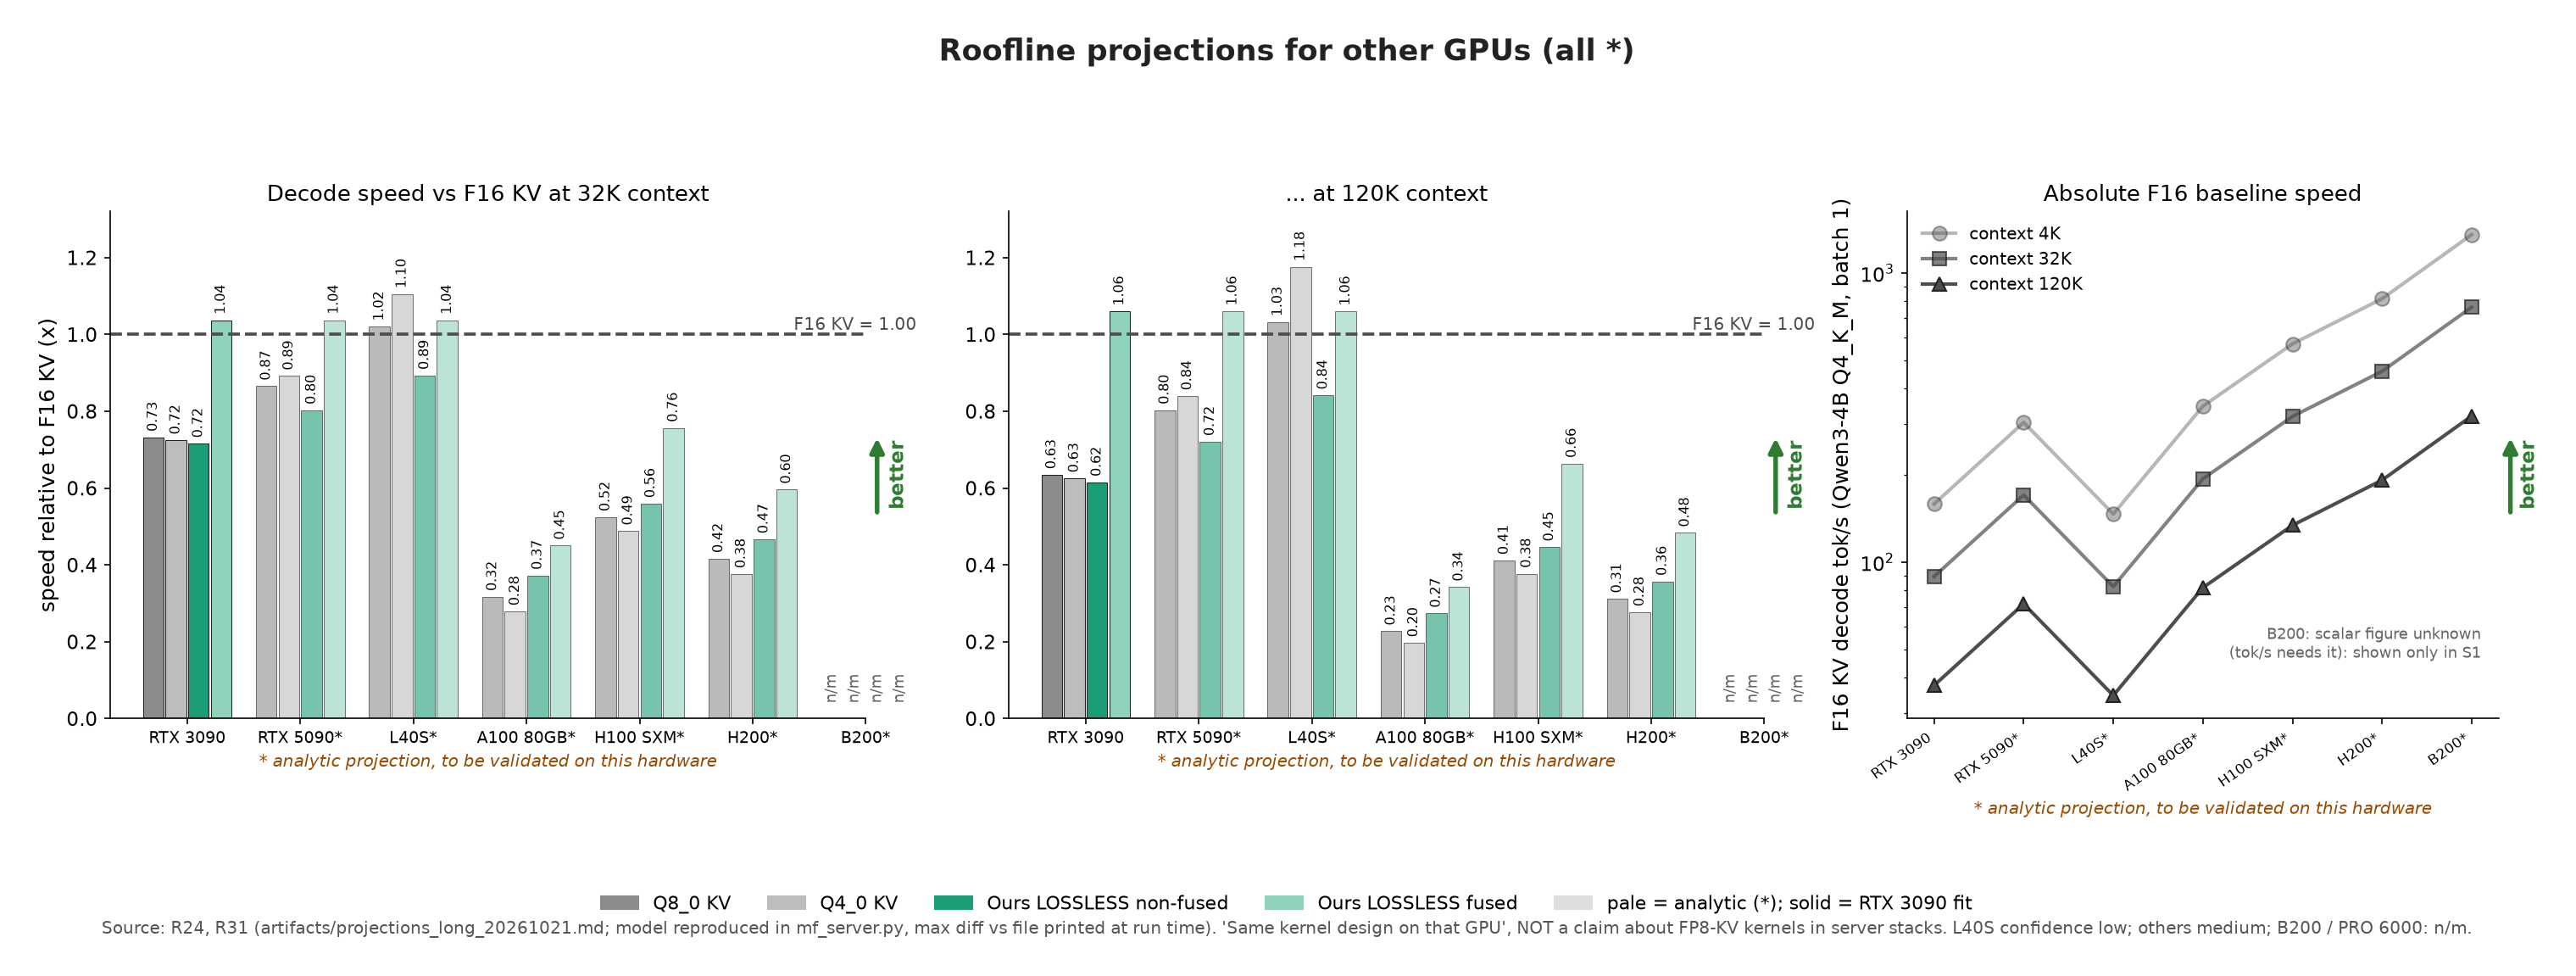
\includegraphics[width=\linewidth]{figures/fig22_server_roofline_projections.png}\caption{\textbf{Figure A1 (*).} Projected decode speed relative to F16 KV at 32K and 120K for llama.cpp-style Q8\_0/Q4\_0 kernels and for our lossless EXP3, non-fused and fused, by card (R24, R31). * analytic projection, to be validated on this hardware. The speed projections assume scalar, llama.cpp-style decode kernels calibrated on the RTX 3090; they say nothing about FP8/INT4 tensor-core kernels of server stacks (vLLM, TensorRT-LLM, SGLang), so they must not be read as "compression loses on servers". Capacity gains are listed separately and do not depend on kernel speed.}\end{figure}

\begin{figure}[htbp]\centering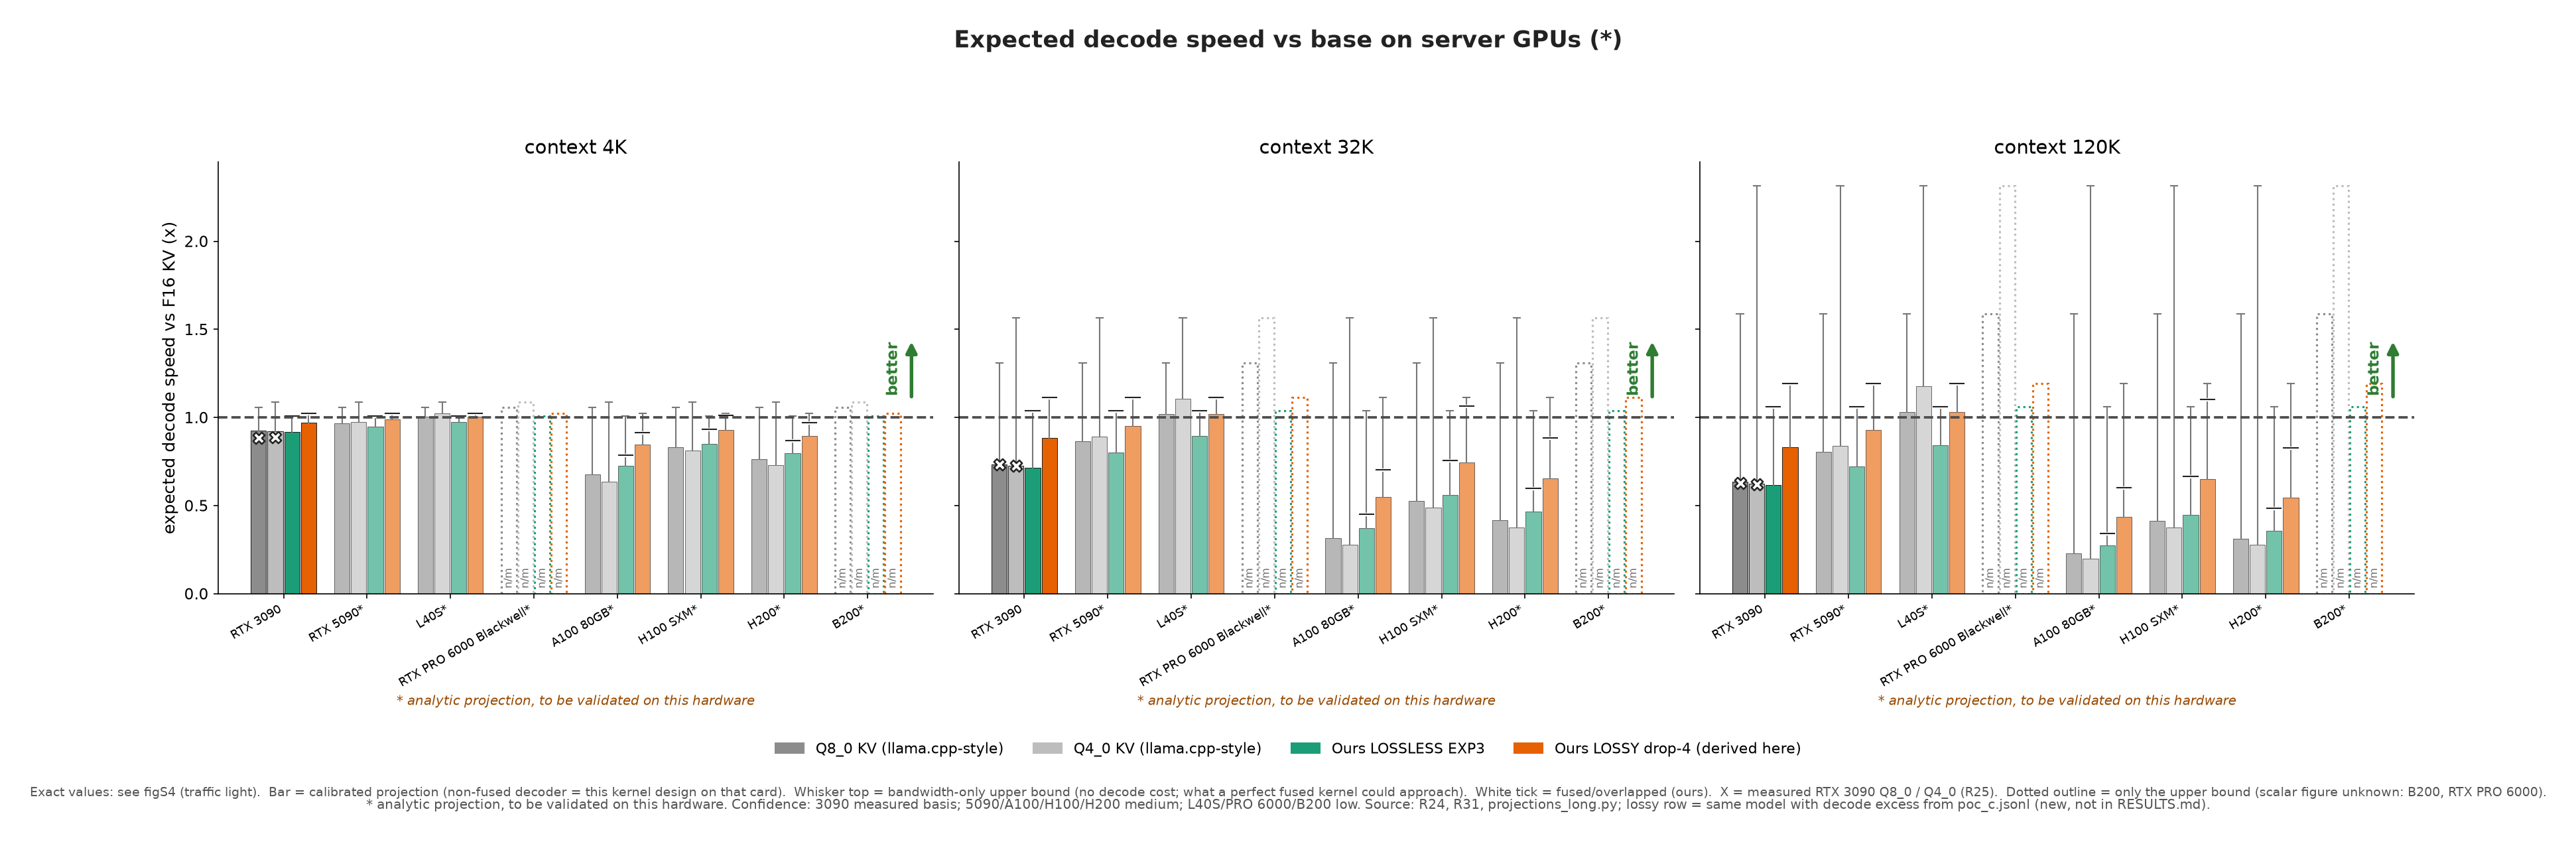
\includegraphics[width=\linewidth]{figures/figS1_server_speedup_by_card_context.png}\caption{\textbf{Figure A2 (*).} Expected decode speed relative to the base by card and context for Q8\_0, Q4\_0, ours lossless EXP3 and ours lossy drop-4. Bar = calibrated scalar non-fused projection; whisker = bandwidth-only upper bound; tick = fused; X = measured on the RTX 3090. * analytic projection, to be validated on this hardware. The speed projections assume scalar, llama.cpp-style decode kernels calibrated on the RTX 3090; they say nothing about FP8/INT4 tensor-core kernels of server stacks (vLLM, TensorRT-LLM, SGLang), so they must not be read as "compression loses on servers". Capacity gains are listed separately and do not depend on kernel speed.}\end{figure}

\begin{figure}[htbp]\centering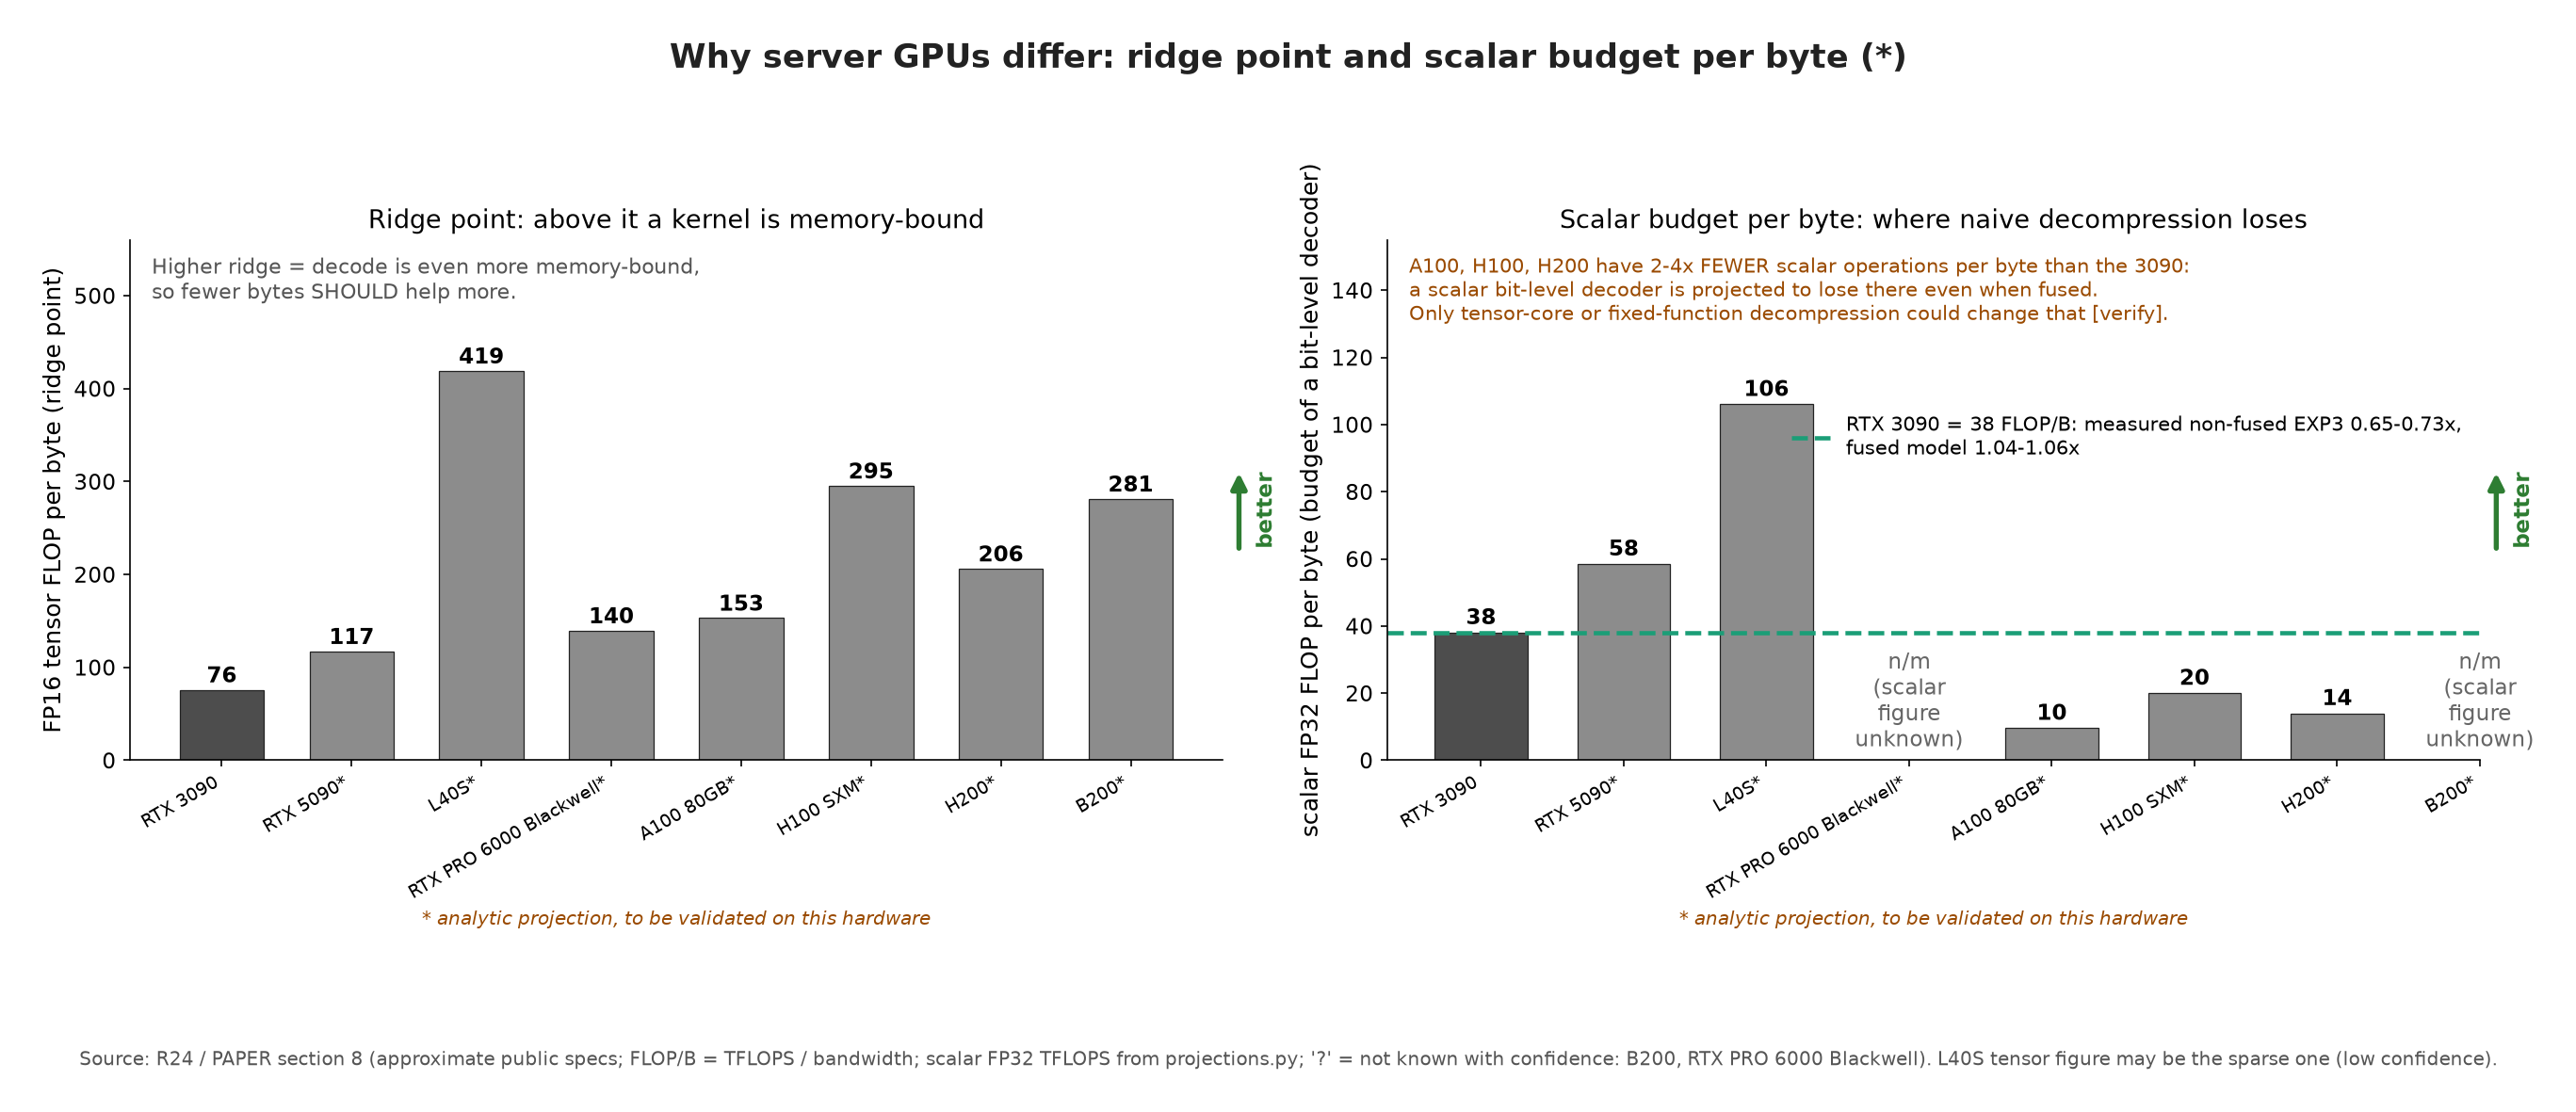
\includegraphics[width=\linewidth]{figures/figS3_ridge_point_and_scalar_budget.png}\caption{\textbf{Figure A3 (*).} Ridge point and scalar FP32 operations per byte by card. A100, H100 and H200 have 2--4$\times$ fewer scalar operations per byte than the RTX 3090, which is why scalar bit-level decoders are projected to lose there; tensor-core or fixed-function decoders are not covered. * analytic projection, to be validated on this hardware. The speed projections assume scalar, llama.cpp-style decode kernels calibrated on the RTX 3090; they say nothing about FP8/INT4 tensor-core kernels of server stacks (vLLM, TensorRT-LLM, SGLang), so they must not be read as "compression loses on servers". Capacity gains are listed separately and do not depend on kernel speed.}\end{figure}

\begin{figure}[htbp]\centering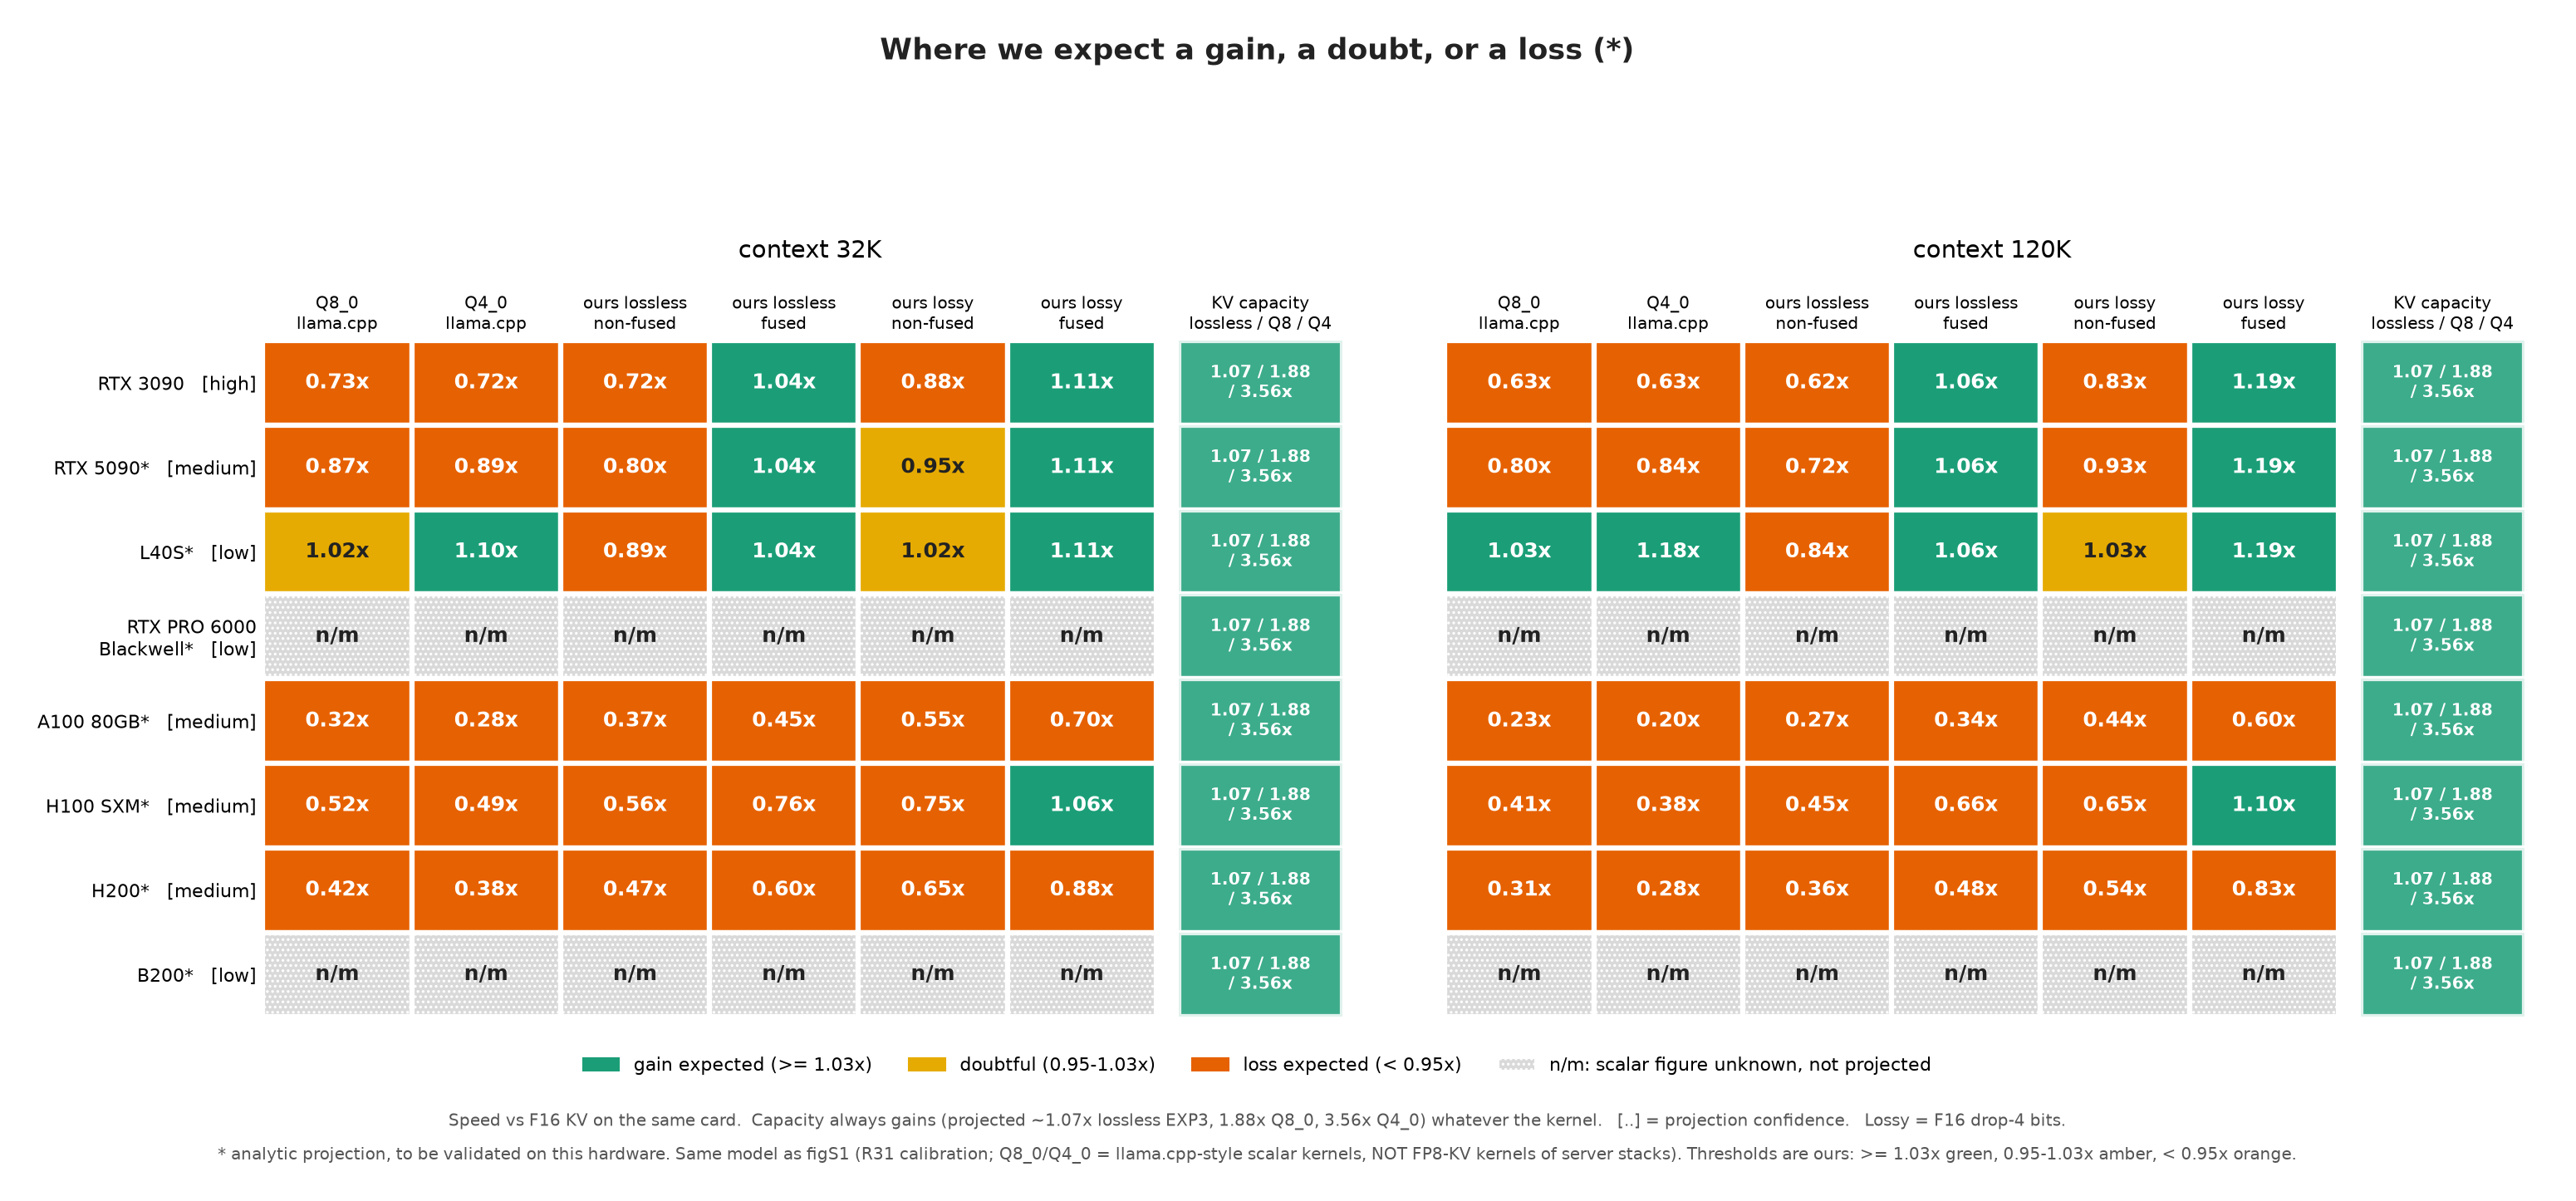
\includegraphics[width=\linewidth]{figures/figS4_server_gain_or_loss_traffic_light.png}\caption{\textbf{Figure A4 (*).} Where a speed gain, a doubt or a loss is projected for scalar llama.cpp-style kernels, by card and format, plus the capacity column. The thresholds ($\geq$ 1.03 gain, 0.95--1.03 doubtful, < 0.95 loss) are ours. * analytic projection, to be validated on this hardware. The speed projections assume scalar, llama.cpp-style decode kernels calibrated on the RTX 3090; they say nothing about FP8/INT4 tensor-core kernels of server stacks (vLLM, TensorRT-LLM, SGLang), so they must not be read as "compression loses on servers". Capacity gains are listed separately and do not depend on kernel speed.}\end{figure}

\textbf{Capacity (independent of kernel speed).}

\begin{figure}[htbp]\centering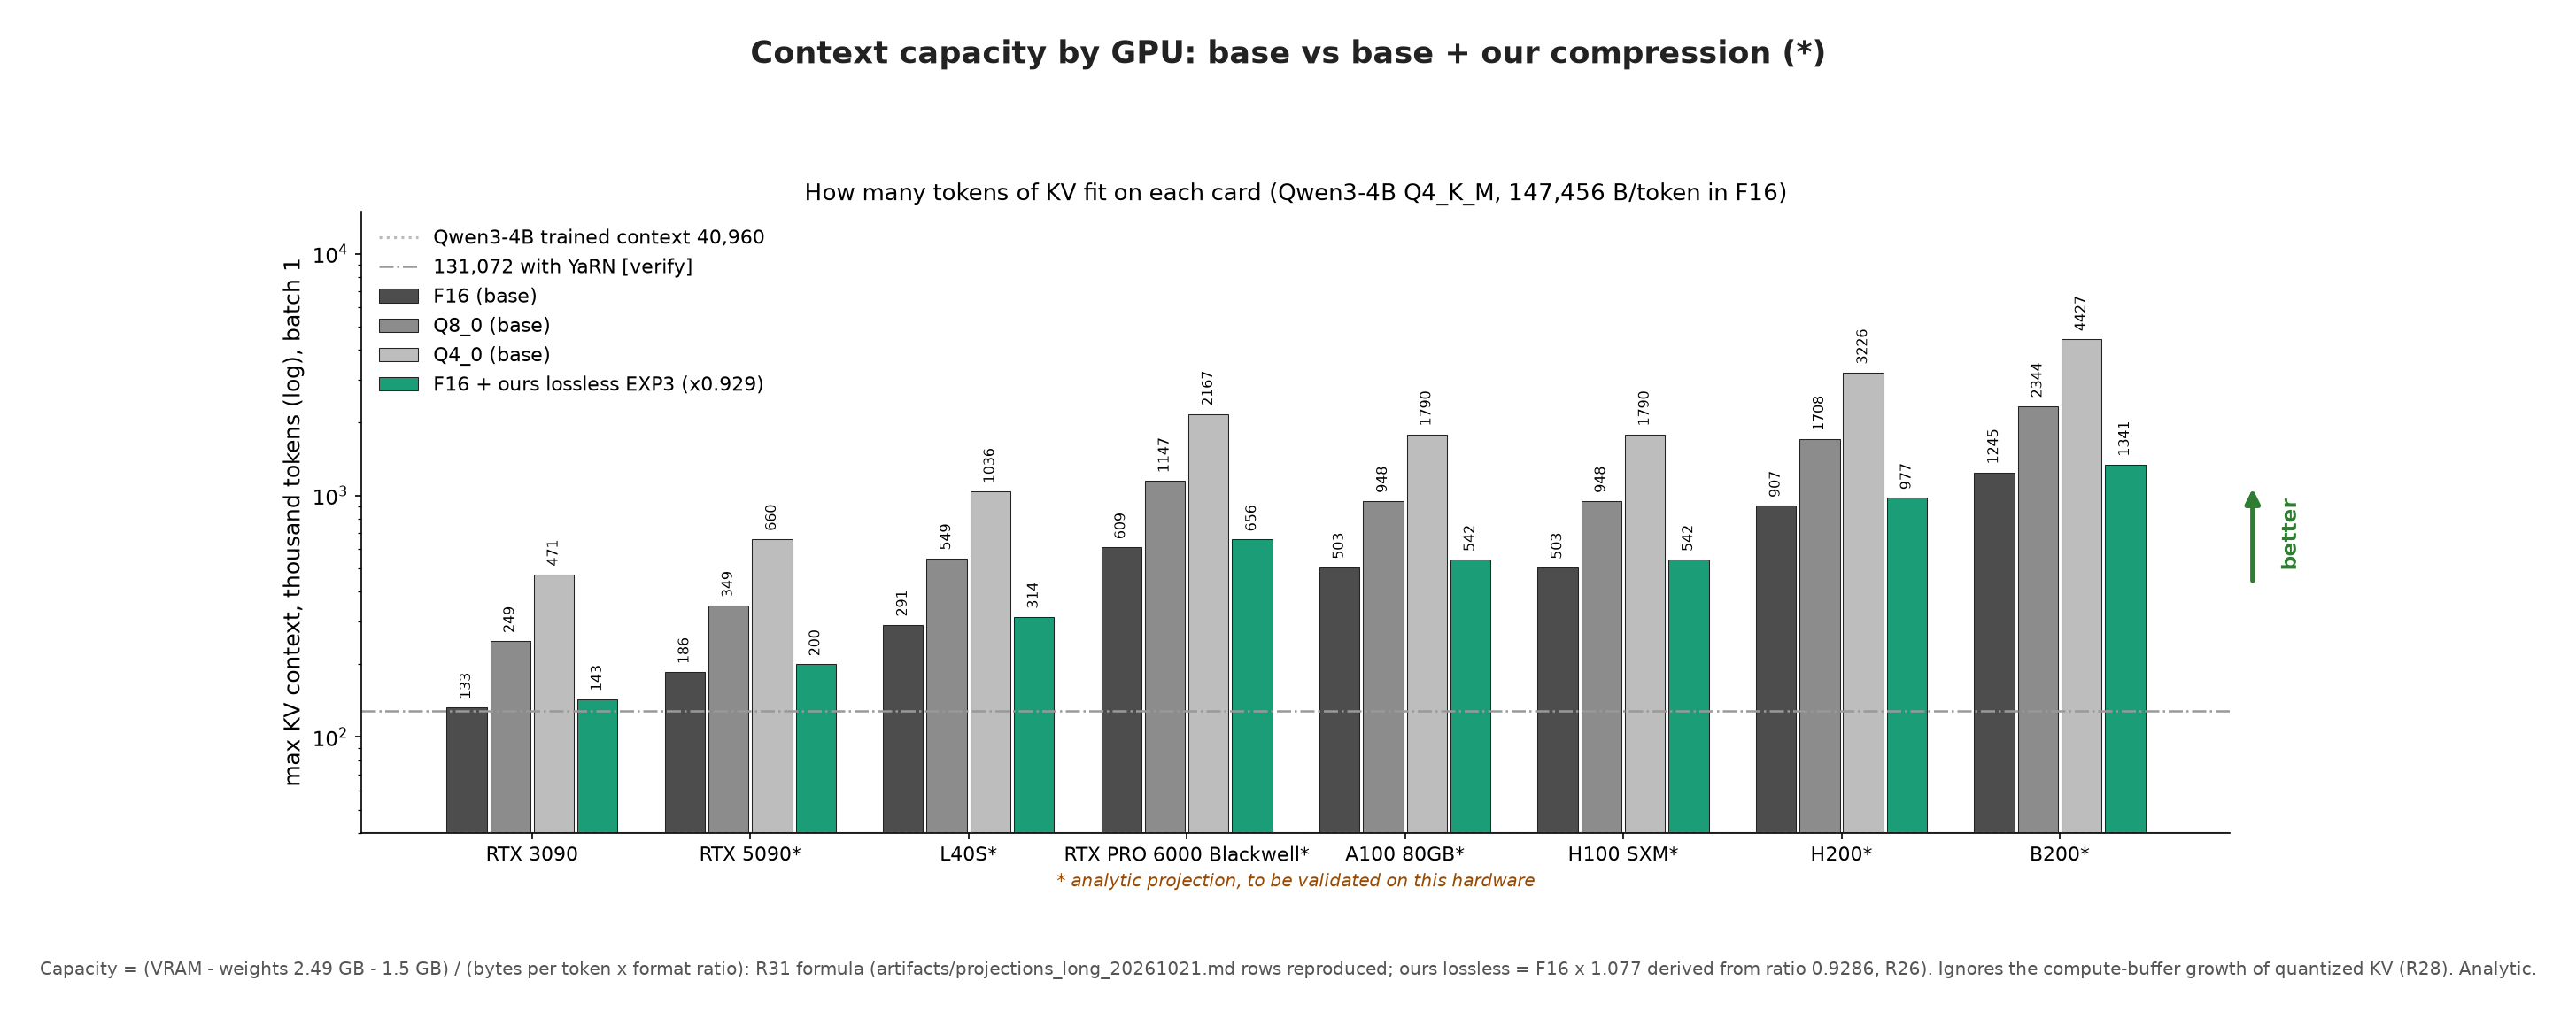
\includegraphics[width=\linewidth]{figures/fig23_context_capacity_by_card.png}\caption{\textbf{Figure A5 (*).} Maximum KV context by card for F16, Q8\_0, Q4\_0 and F16 + EXP3 at batch 1 (R31 formula; Qwen3-4B, 147,456 bytes per token in F16). * analytic projection, to be validated on this hardware. The speed projections assume scalar, llama.cpp-style decode kernels calibrated on the RTX 3090; they say nothing about FP8/INT4 tensor-core kernels of server stacks (vLLM, TensorRT-LLM, SGLang), so they must not be read as "compression loses on servers". Capacity gains are listed separately and do not depend on kernel speed.}\end{figure}

\begin{figure}[htbp]\centering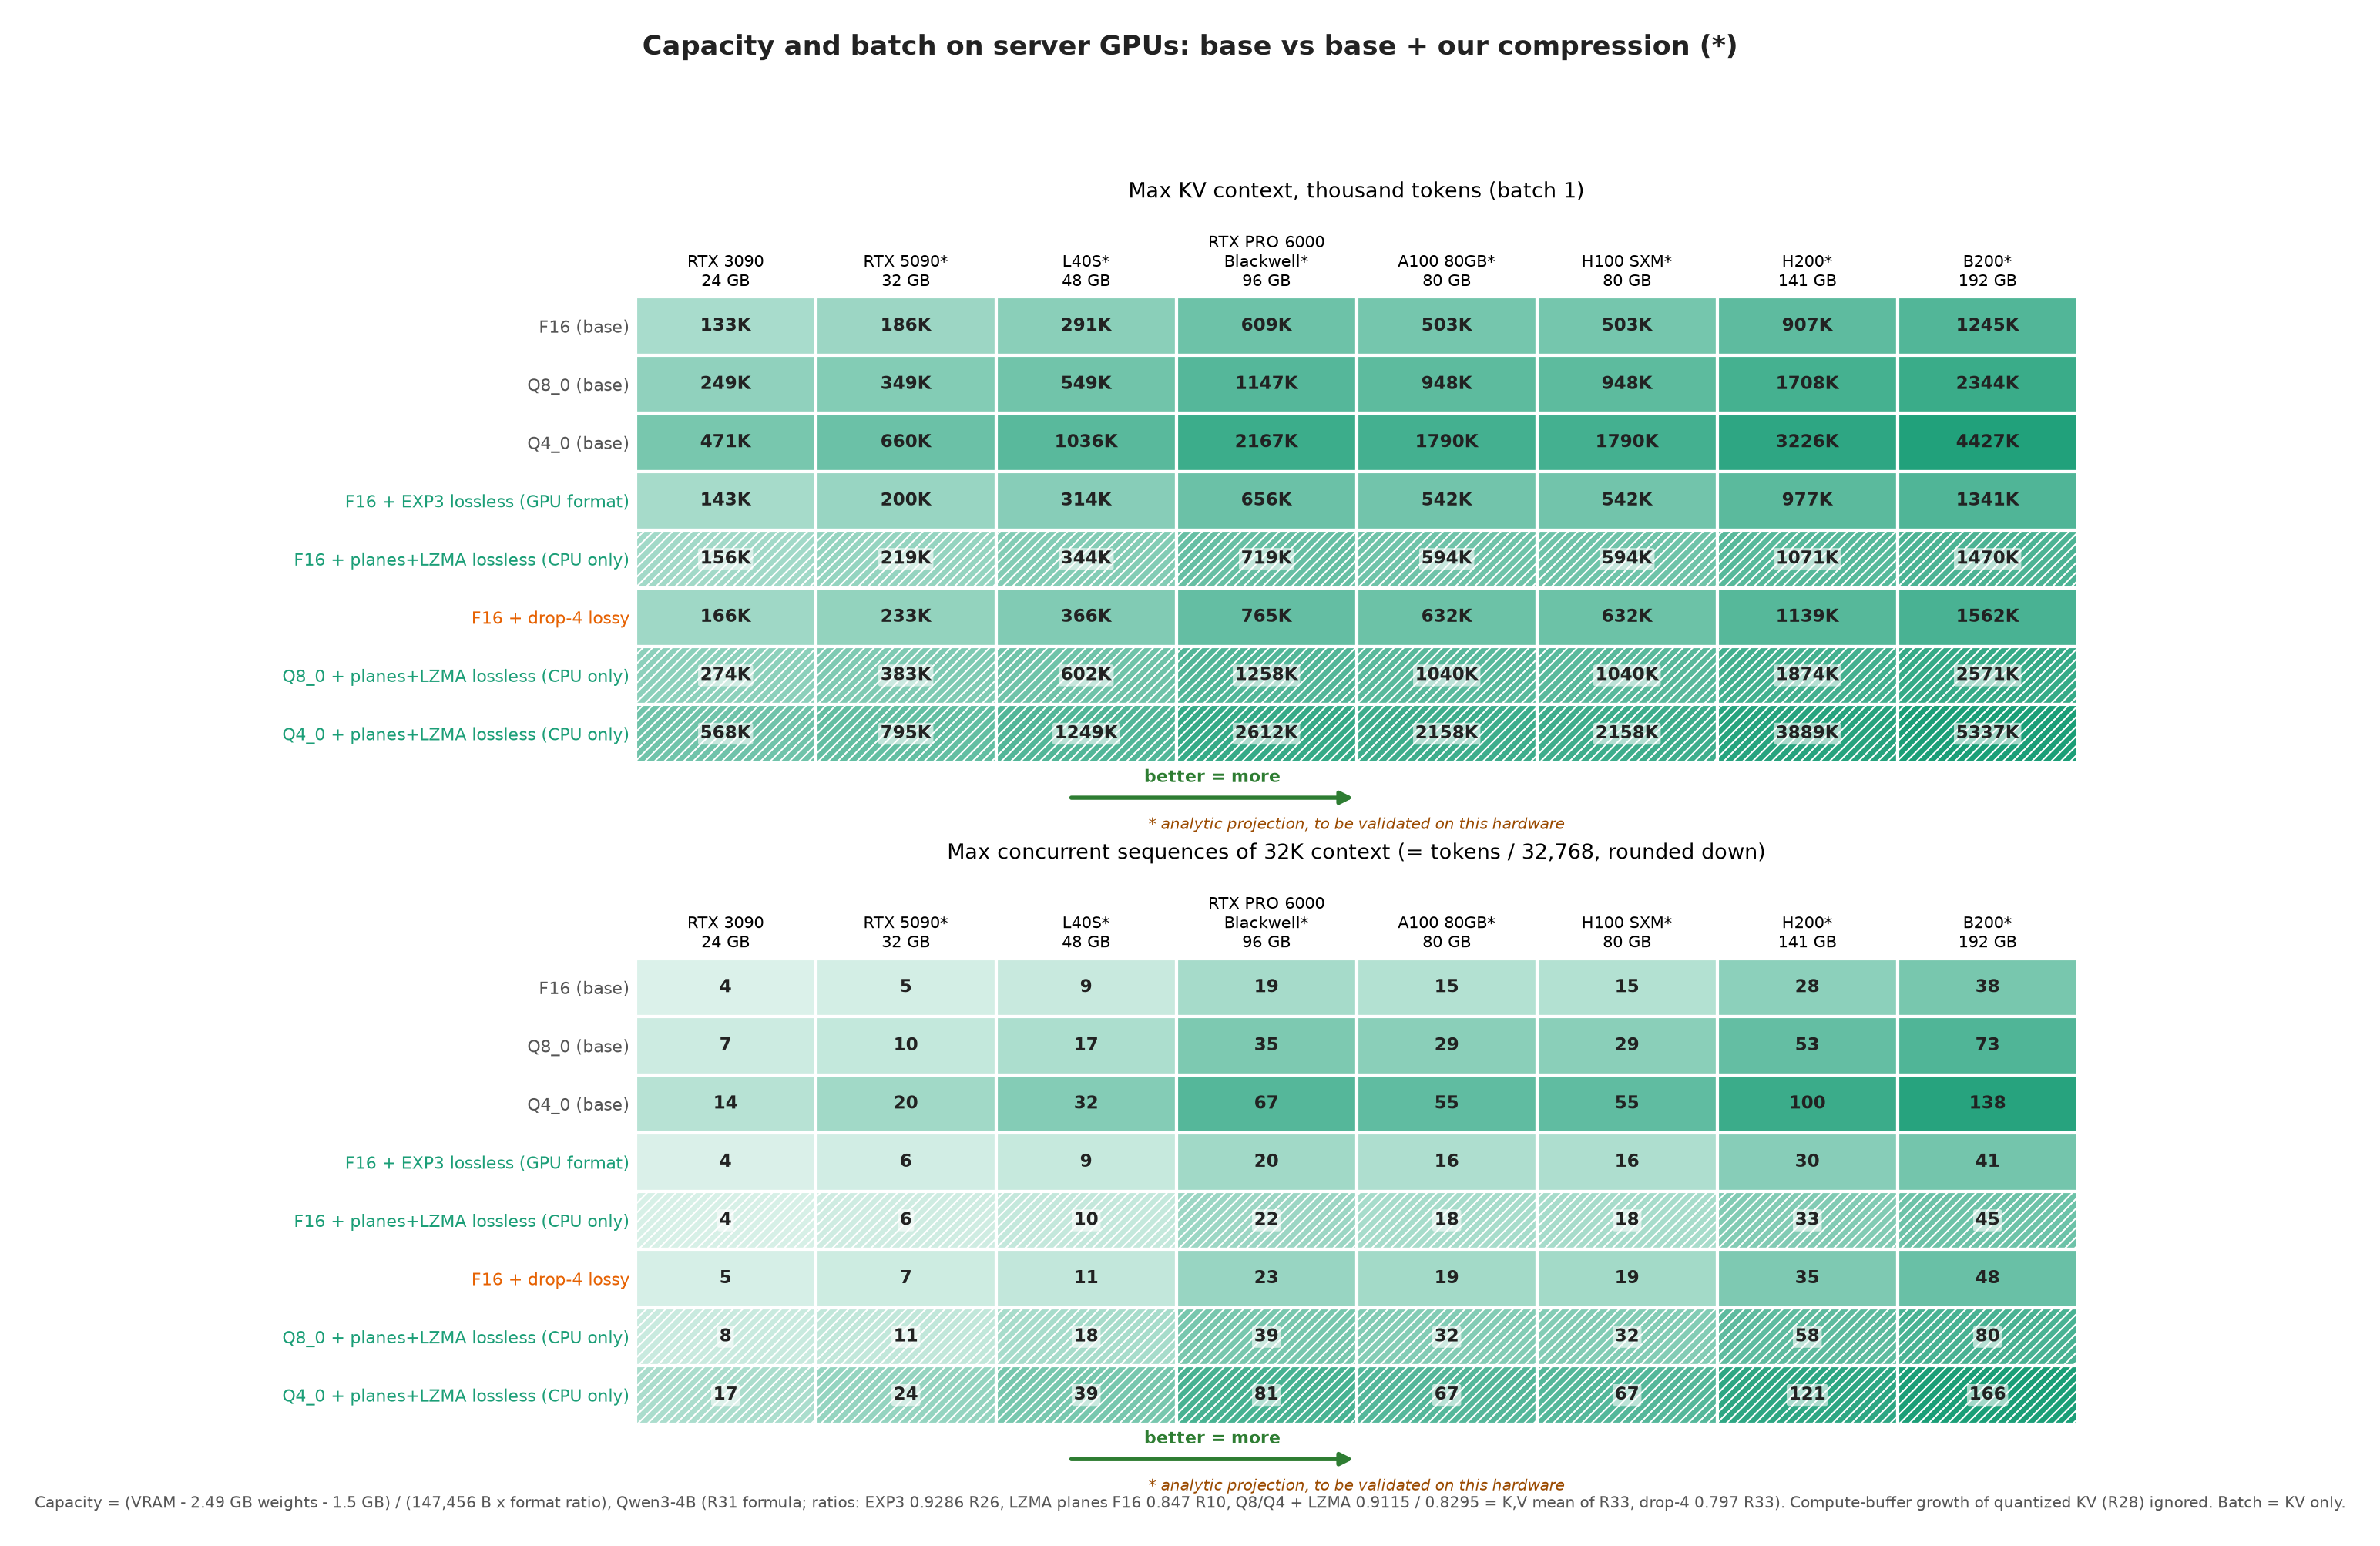
\includegraphics[width=\linewidth]{figures/figS2_server_capacity_and_max_batch.png}\caption{\textbf{Figure A6 (*).} Maximum context and maximum number of concurrent 32K sequences, base vs base + our compression. The batch count covers KV only and ignores activations and the compute-buffer growth of quantized KV (R28). * analytic projection, to be validated on this hardware. The speed projections assume scalar, llama.cpp-style decode kernels calibrated on the RTX 3090; they say nothing about FP8/INT4 tensor-core kernels of server stacks (vLLM, TensorRT-LLM, SGLang), so they must not be read as "compression loses on servers". Capacity gains are listed separately and do not depend on kernel speed.}\end{figure}

\begin{figure}[htbp]\centering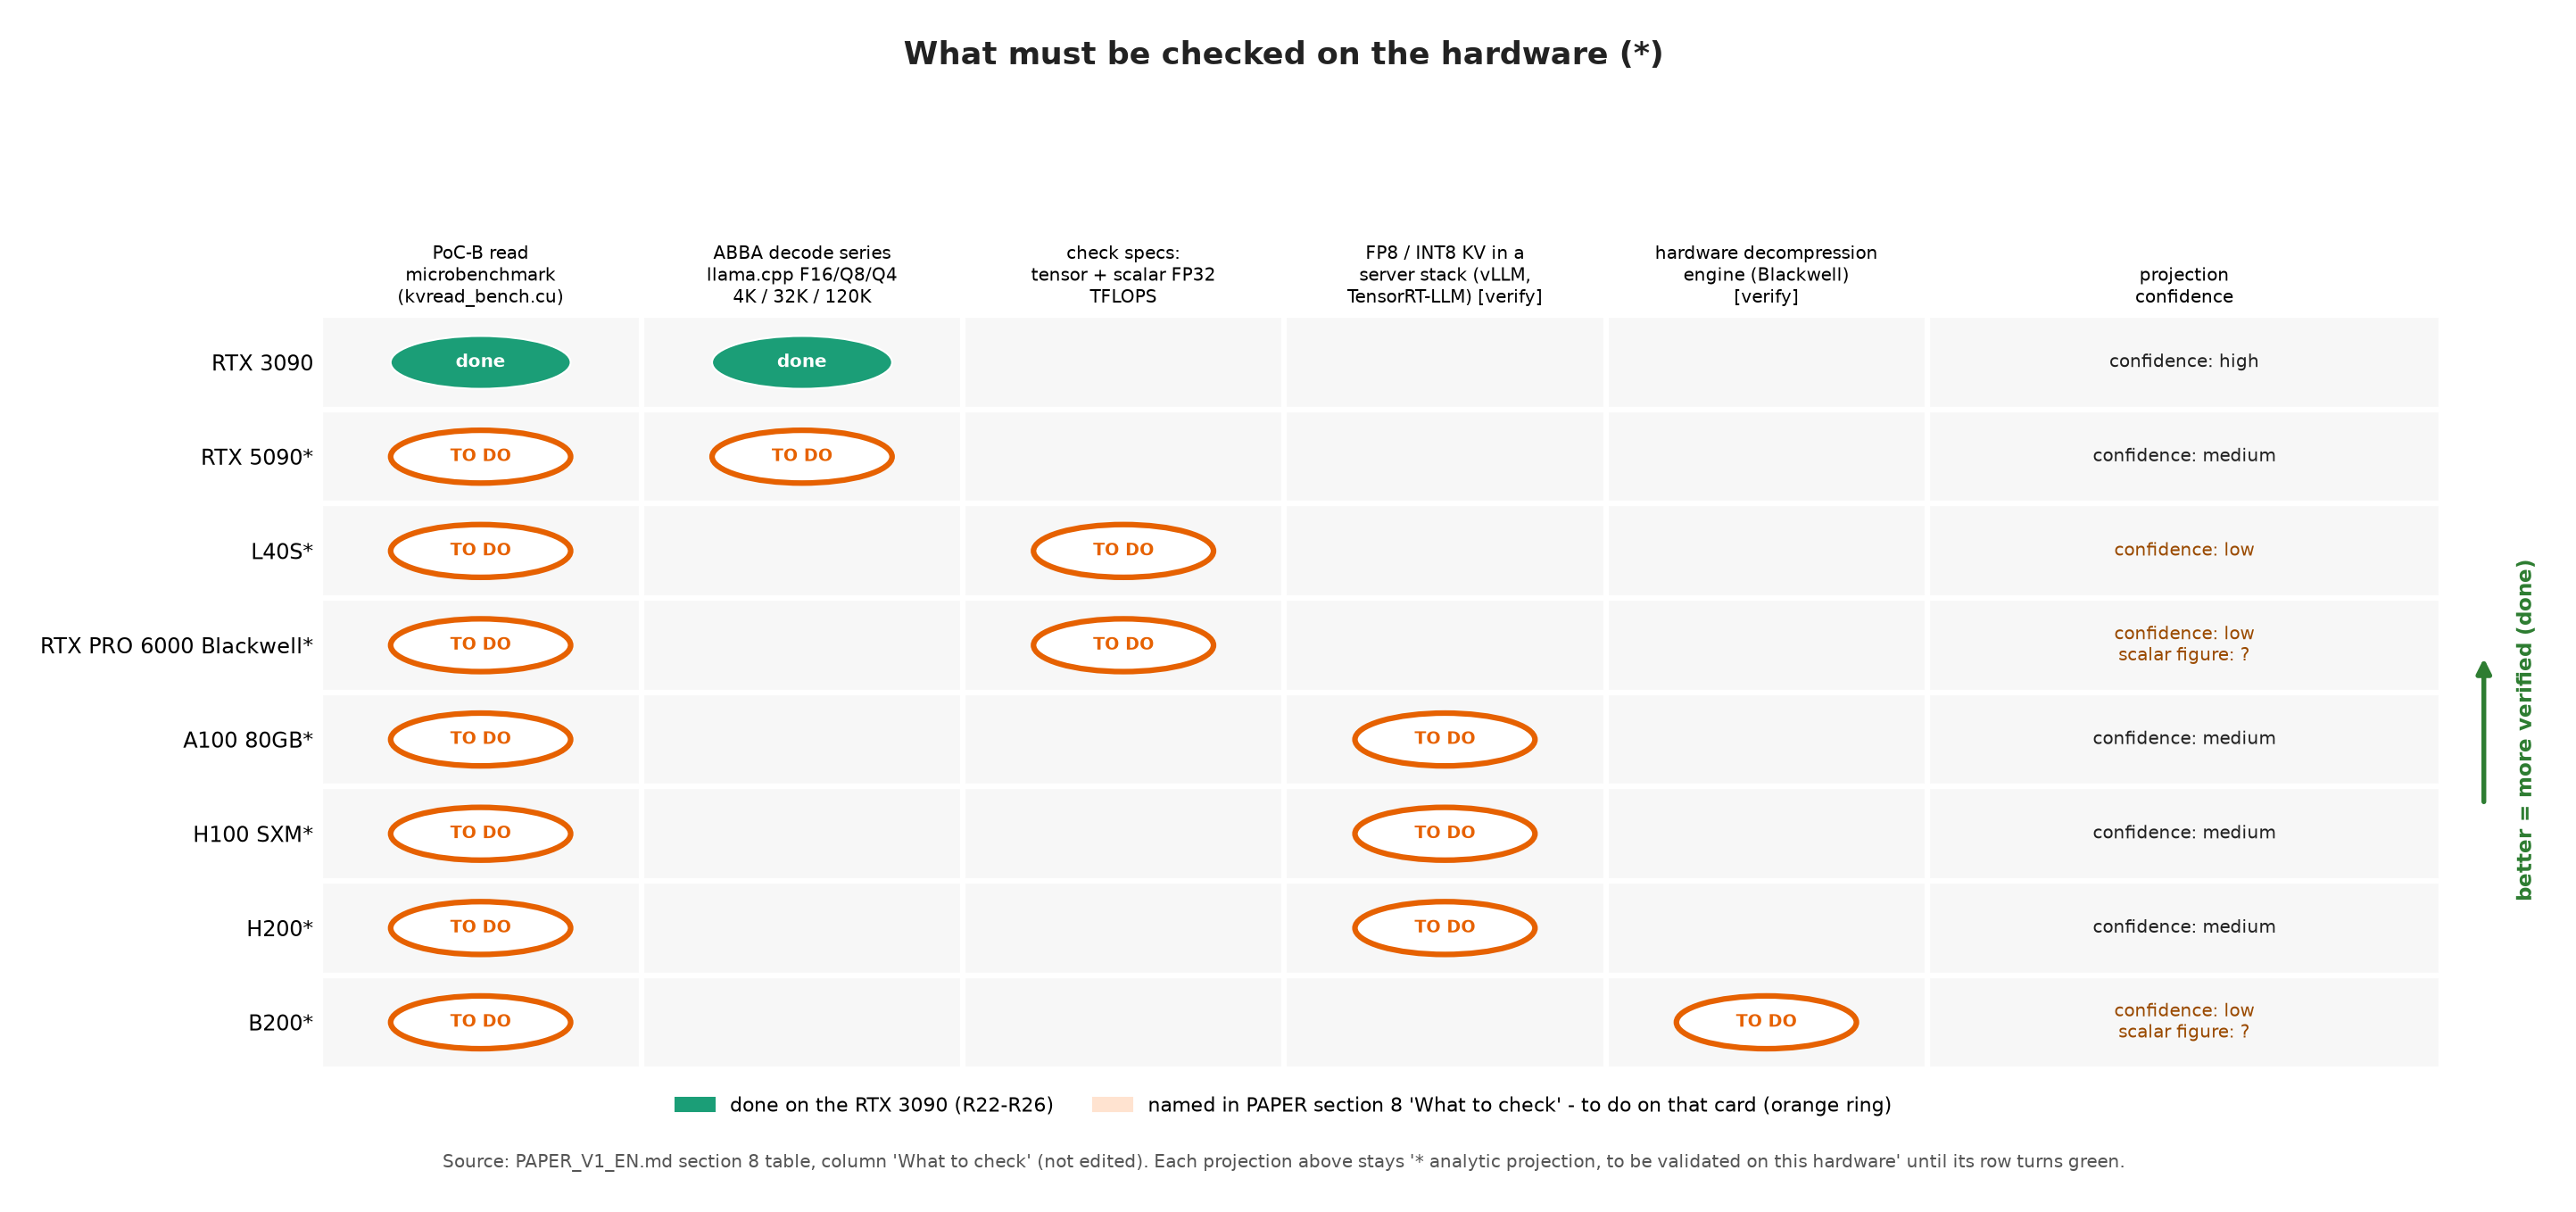
\includegraphics[width=\linewidth]{figures/figS5_hardware_validation_checklist.png}\caption{\textbf{Figure A7 (*).} What must be measured on each card before any projection is trusted. Only the RTX 3090 is done.}\end{figure}


\section{Reproducibility}

\texttt{release/} holds the scripts, the PoC CUDA sources, the llama.cpp patch (\texttt{patches/}) and data summaries. Every
table row maps to a file under \texttt{data/}. The fork of Section 7: \texttt{artifacts/fork\_patches/kv/} (7 patches, branch
\texttt{cq/kv-compress}), \texttt{artifacts/fork\_patches/weights/} (3 patches, \texttt{cq/weights-compress}) and
\texttt{artifacts/fork\_patches/combined/} (merge resolution, \texttt{llama-cq-logits --kv}, and the full diff against
\texttt{ed7ac35e}); measurement scripts \texttt{scripts/combo\_*.sh}, summaries \texttt{scripts/combo\_summarize.py}, figures
\texttt{scripts/make\_figures\_combo.py}.

\section{Additional figures}

Colour code: grey = base, green = ours lossless, orange = ours lossy, hatched = CPU prototype only, n/m = not measured.

\begin{figure}[htbp]\centering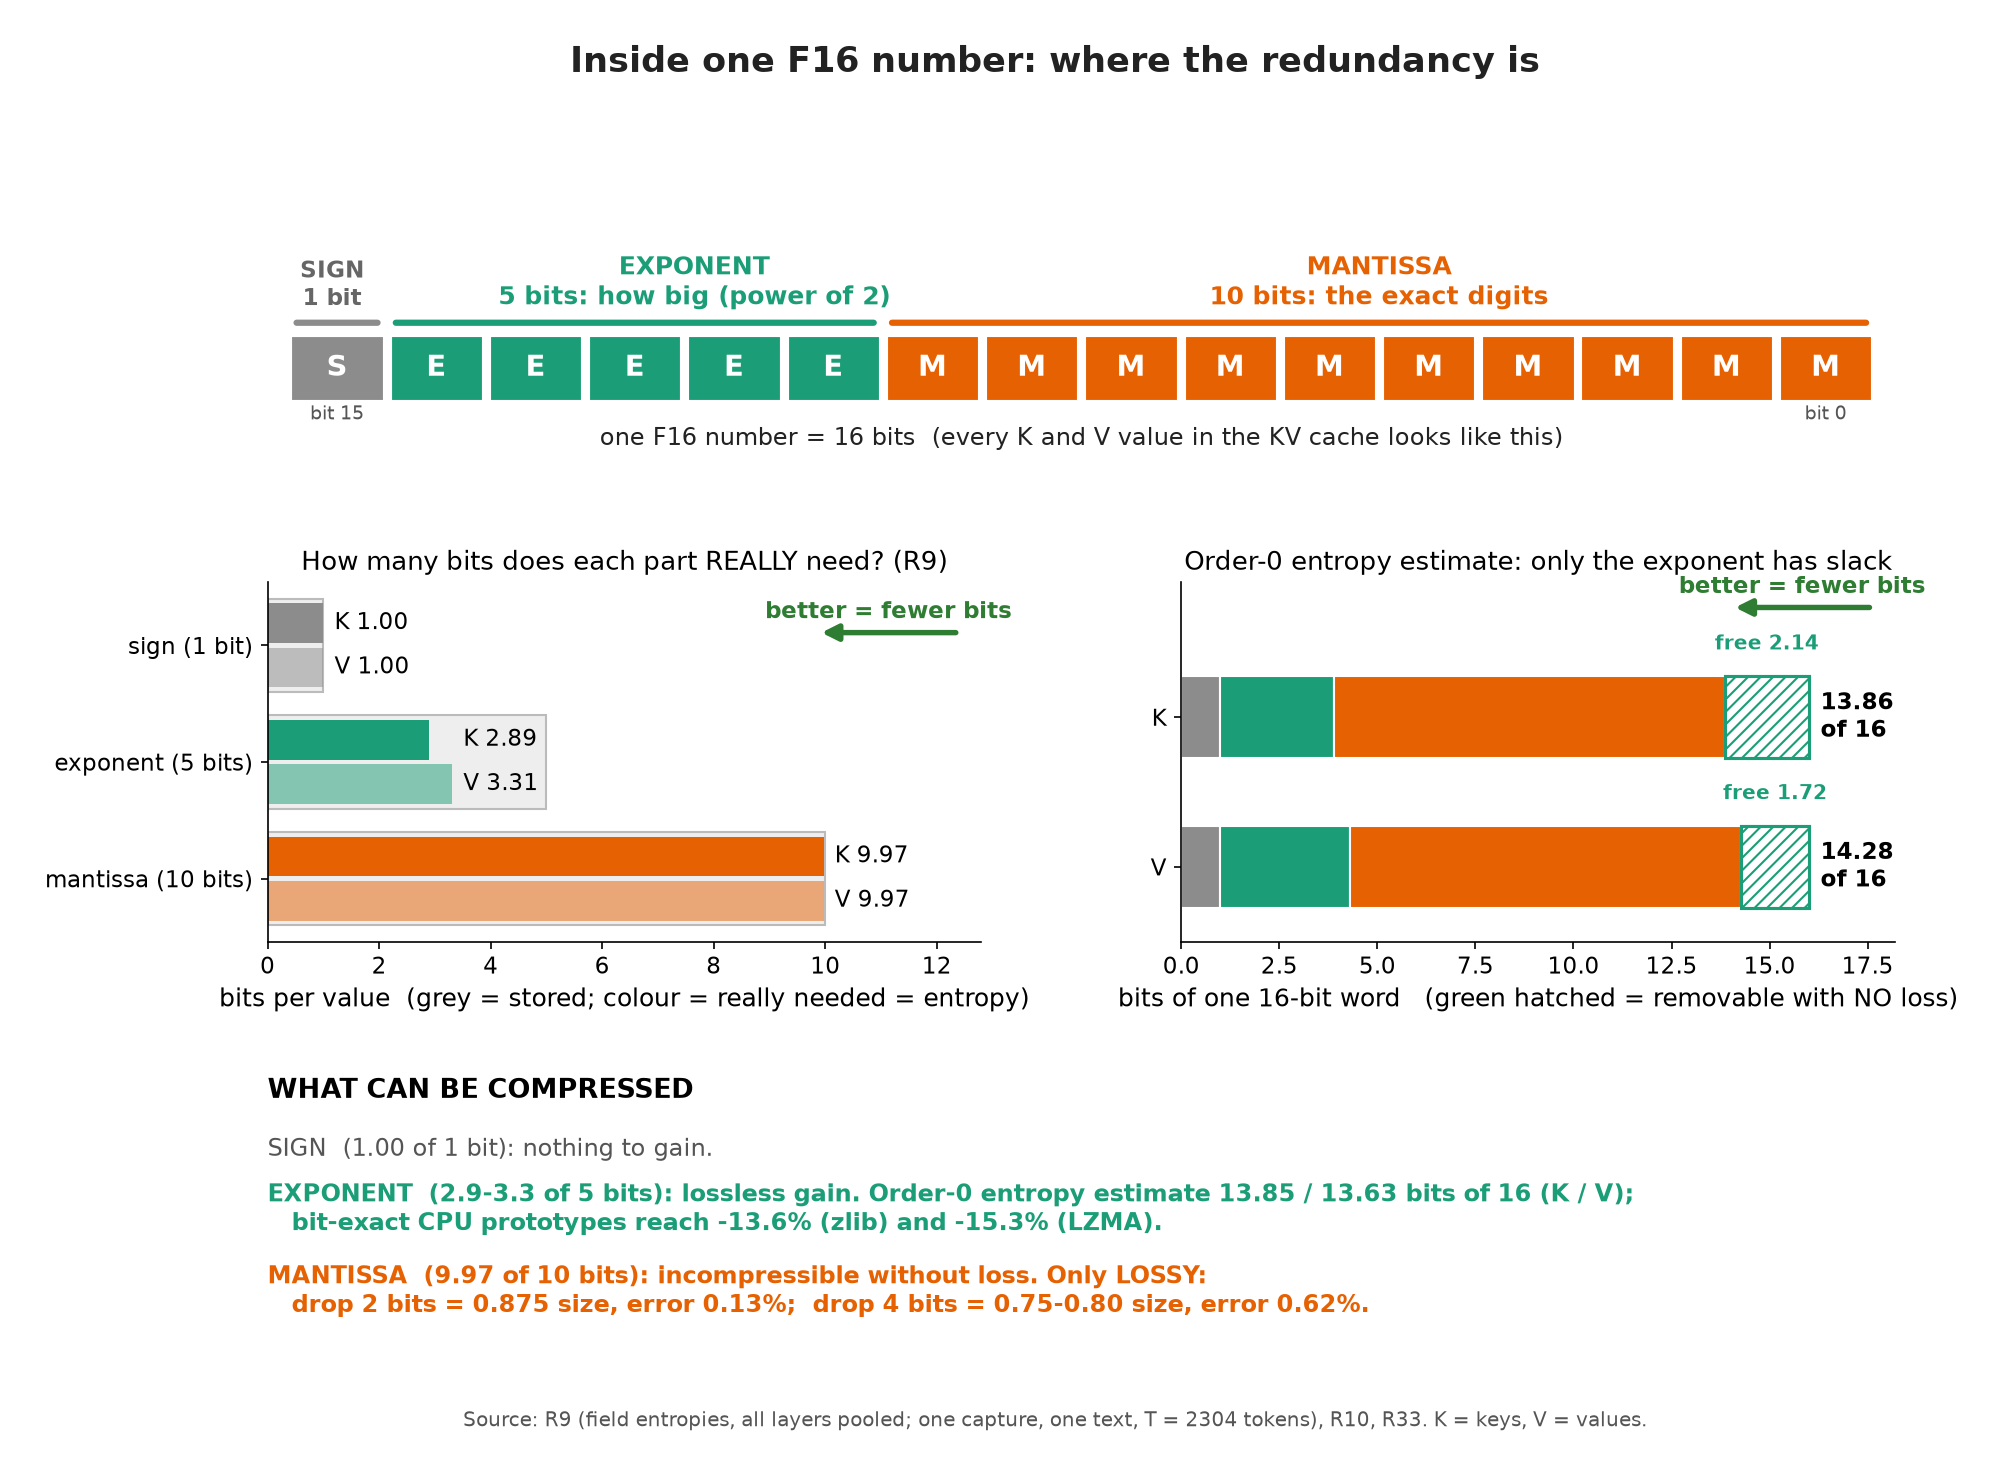
\includegraphics[width=\linewidth]{figures/fig11_fp16_bit_layout.png}\caption{The F16 word: the sign carries 1.00 of 1 bit, the exponent 2.89 (K) and 3.31 (V) of 5 bits order-0, the mantissa 9.97 of 10 bits (R9). Only the exponent can be shrunk without loss.}\end{figure}

\begin{figure}[htbp]\centering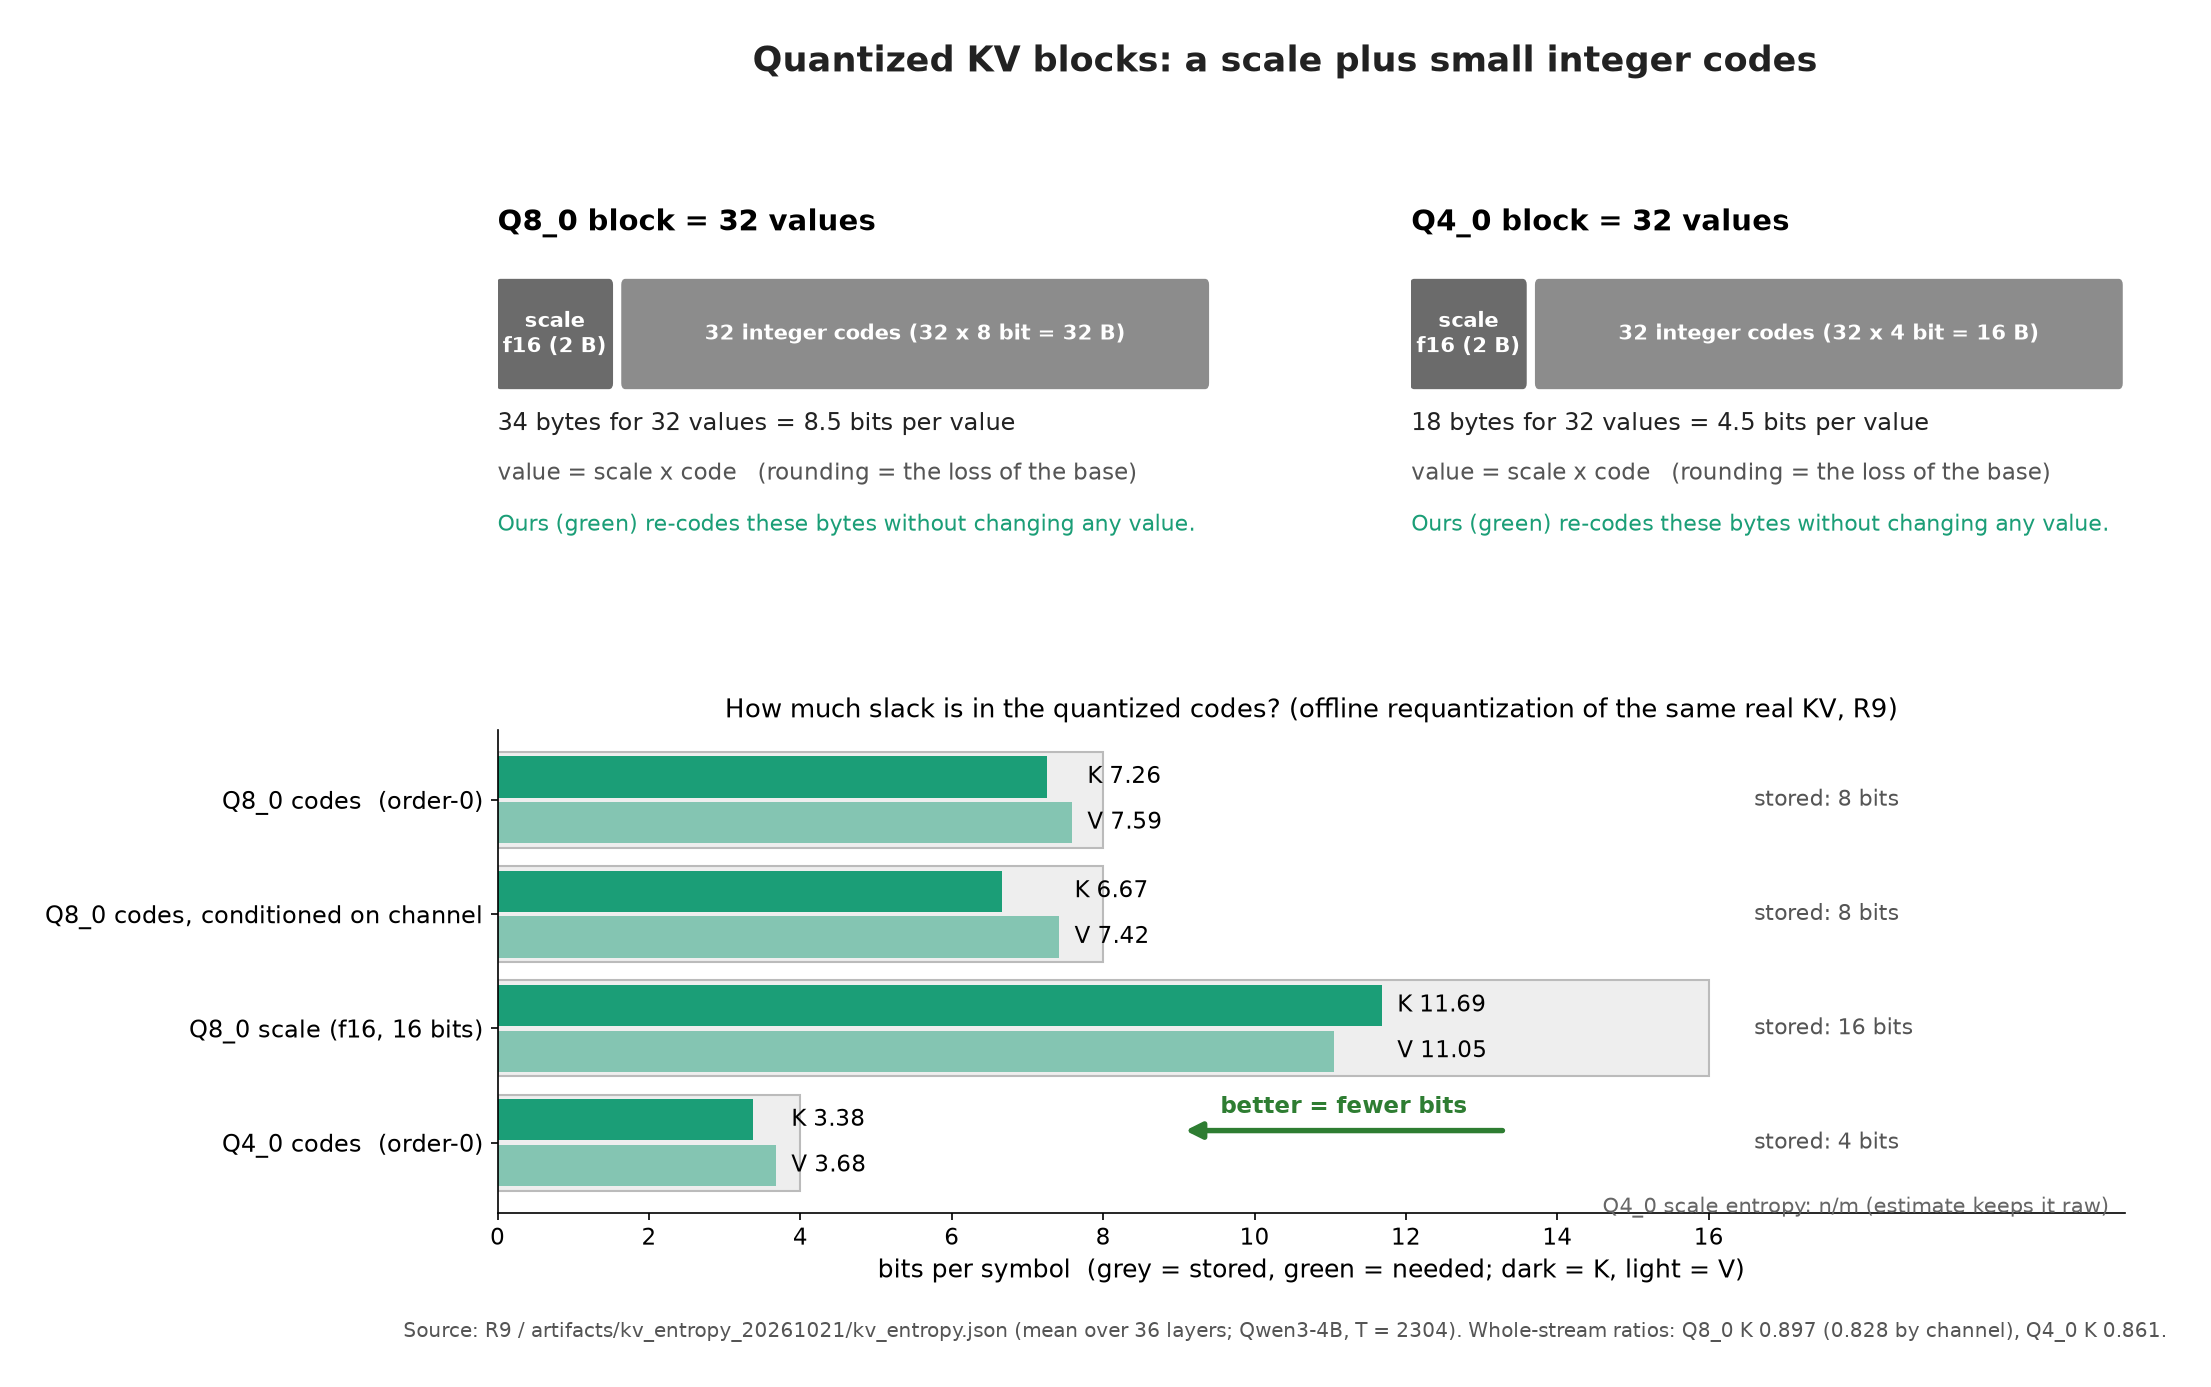
\includegraphics[width=\linewidth]{figures/fig12_q8_q4_blocks_entropy.png}\caption{Q8\_0 and Q4\_0 blocks: the integer codes use 7.3 of 8 and 3.4 of 4 bits (K); the f16 scale of Q8\_0 uses 11.7 of 16 bits (R9).}\end{figure}

\begin{figure}[htbp]\centering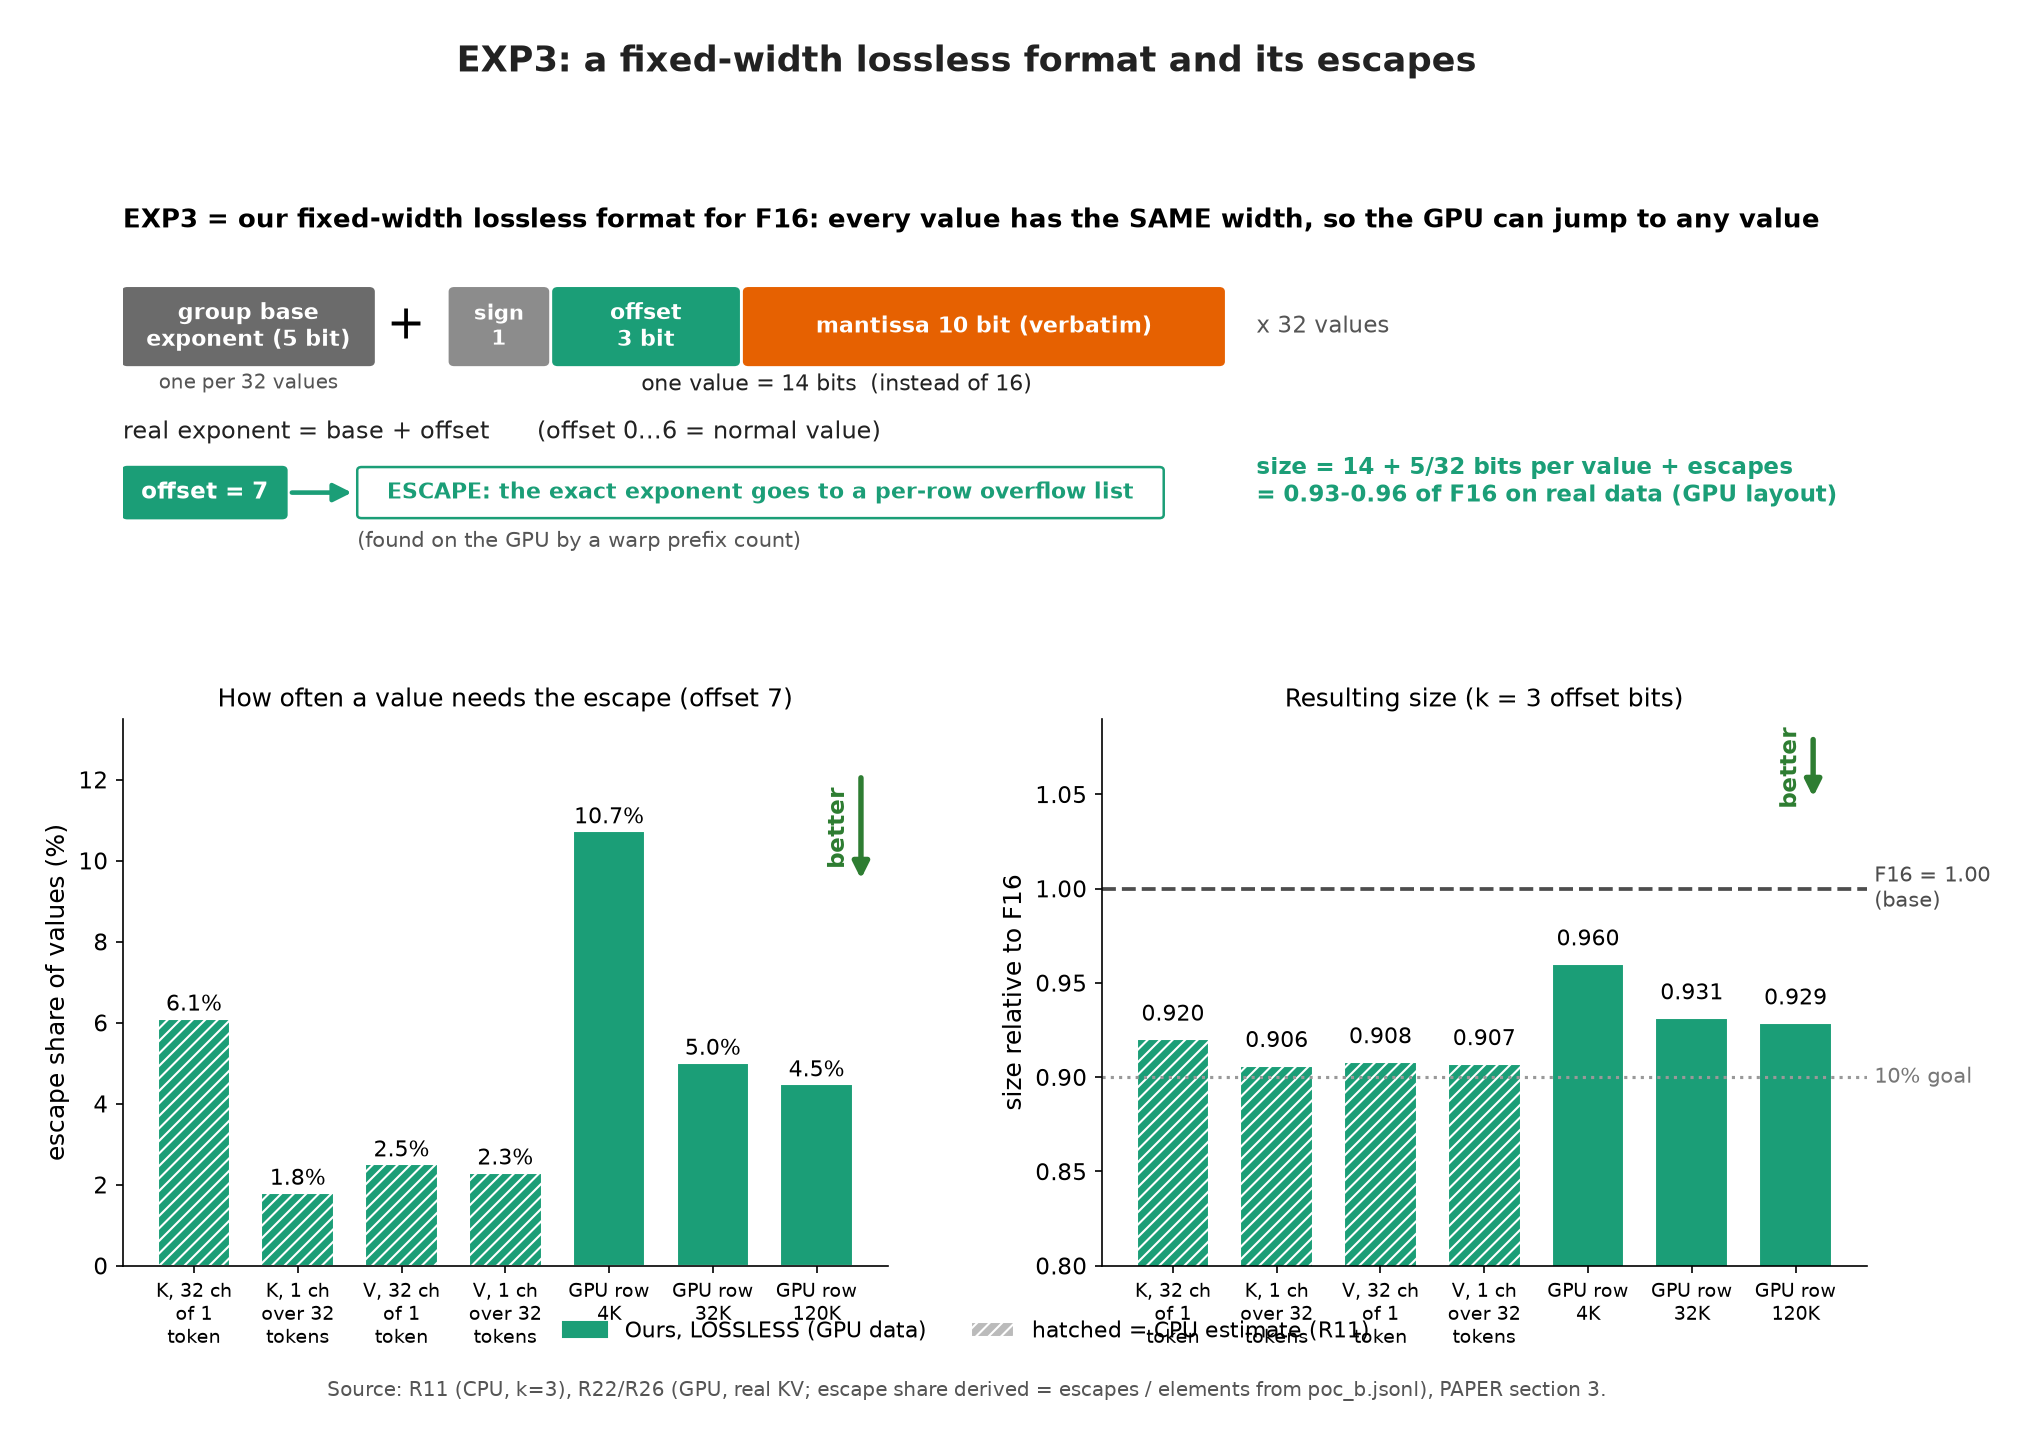
\includegraphics[width=\linewidth]{figures/fig13_exp3_format_escapes.png}\caption{The fixed-rate lossless format EXP3 and the share of values that need the escape: 1.8--6.1\% in CPU groupings, 4.5--10.7\% in the GPU row layout (R11, R26).}\end{figure}

\begin{figure}[htbp]\centering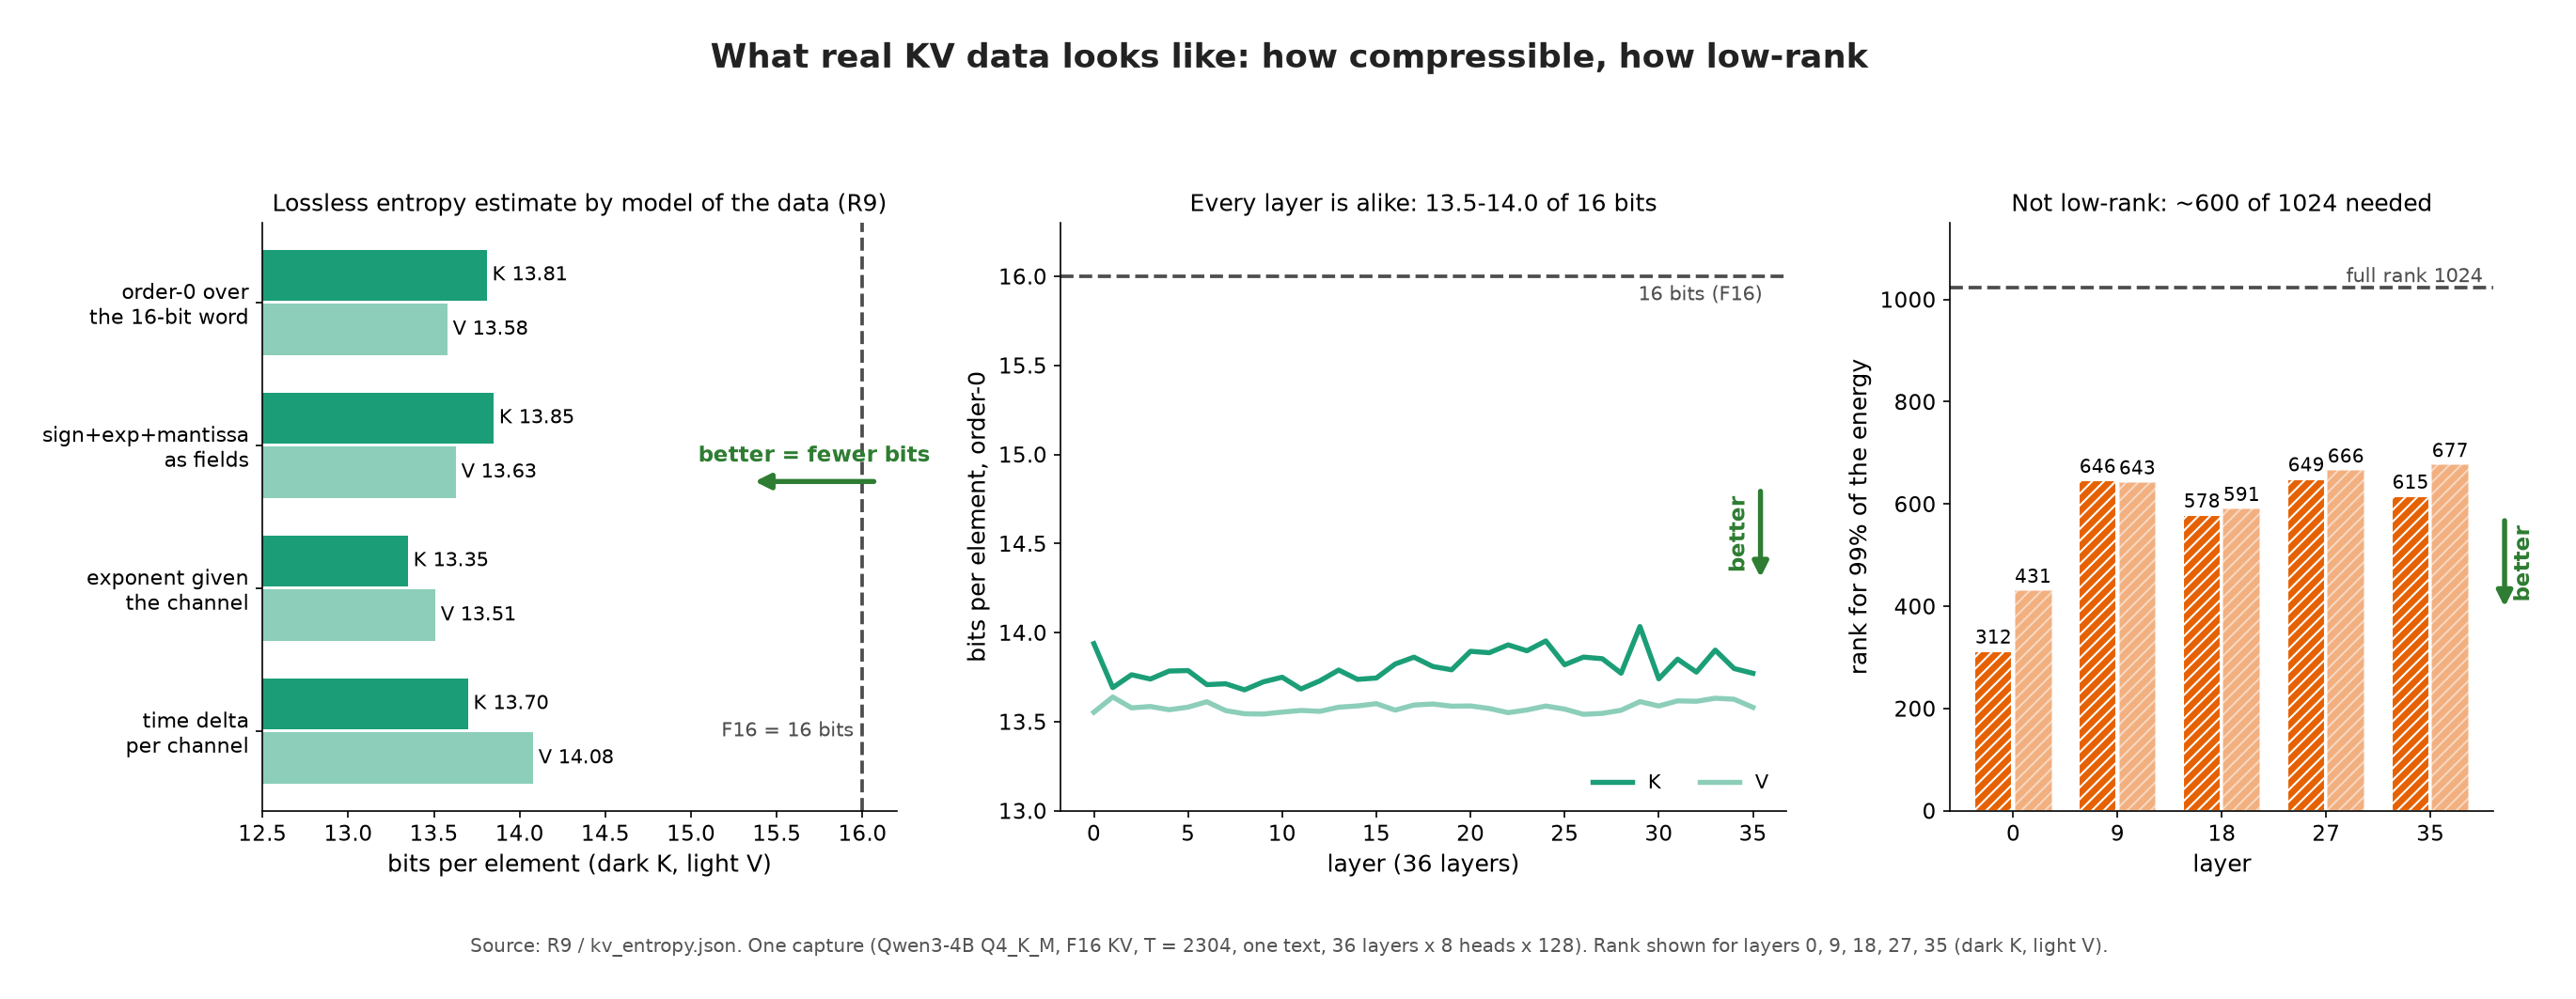
\includegraphics[width=\linewidth]{figures/fig40_real_kv_structure.png}\caption{Real Qwen3-4B KV: entropy by data model, per layer, and SVD rank (about 600 of 1024 directions for 99\% of the energy) (R9).}\end{figure}

\begin{figure}[htbp]\centering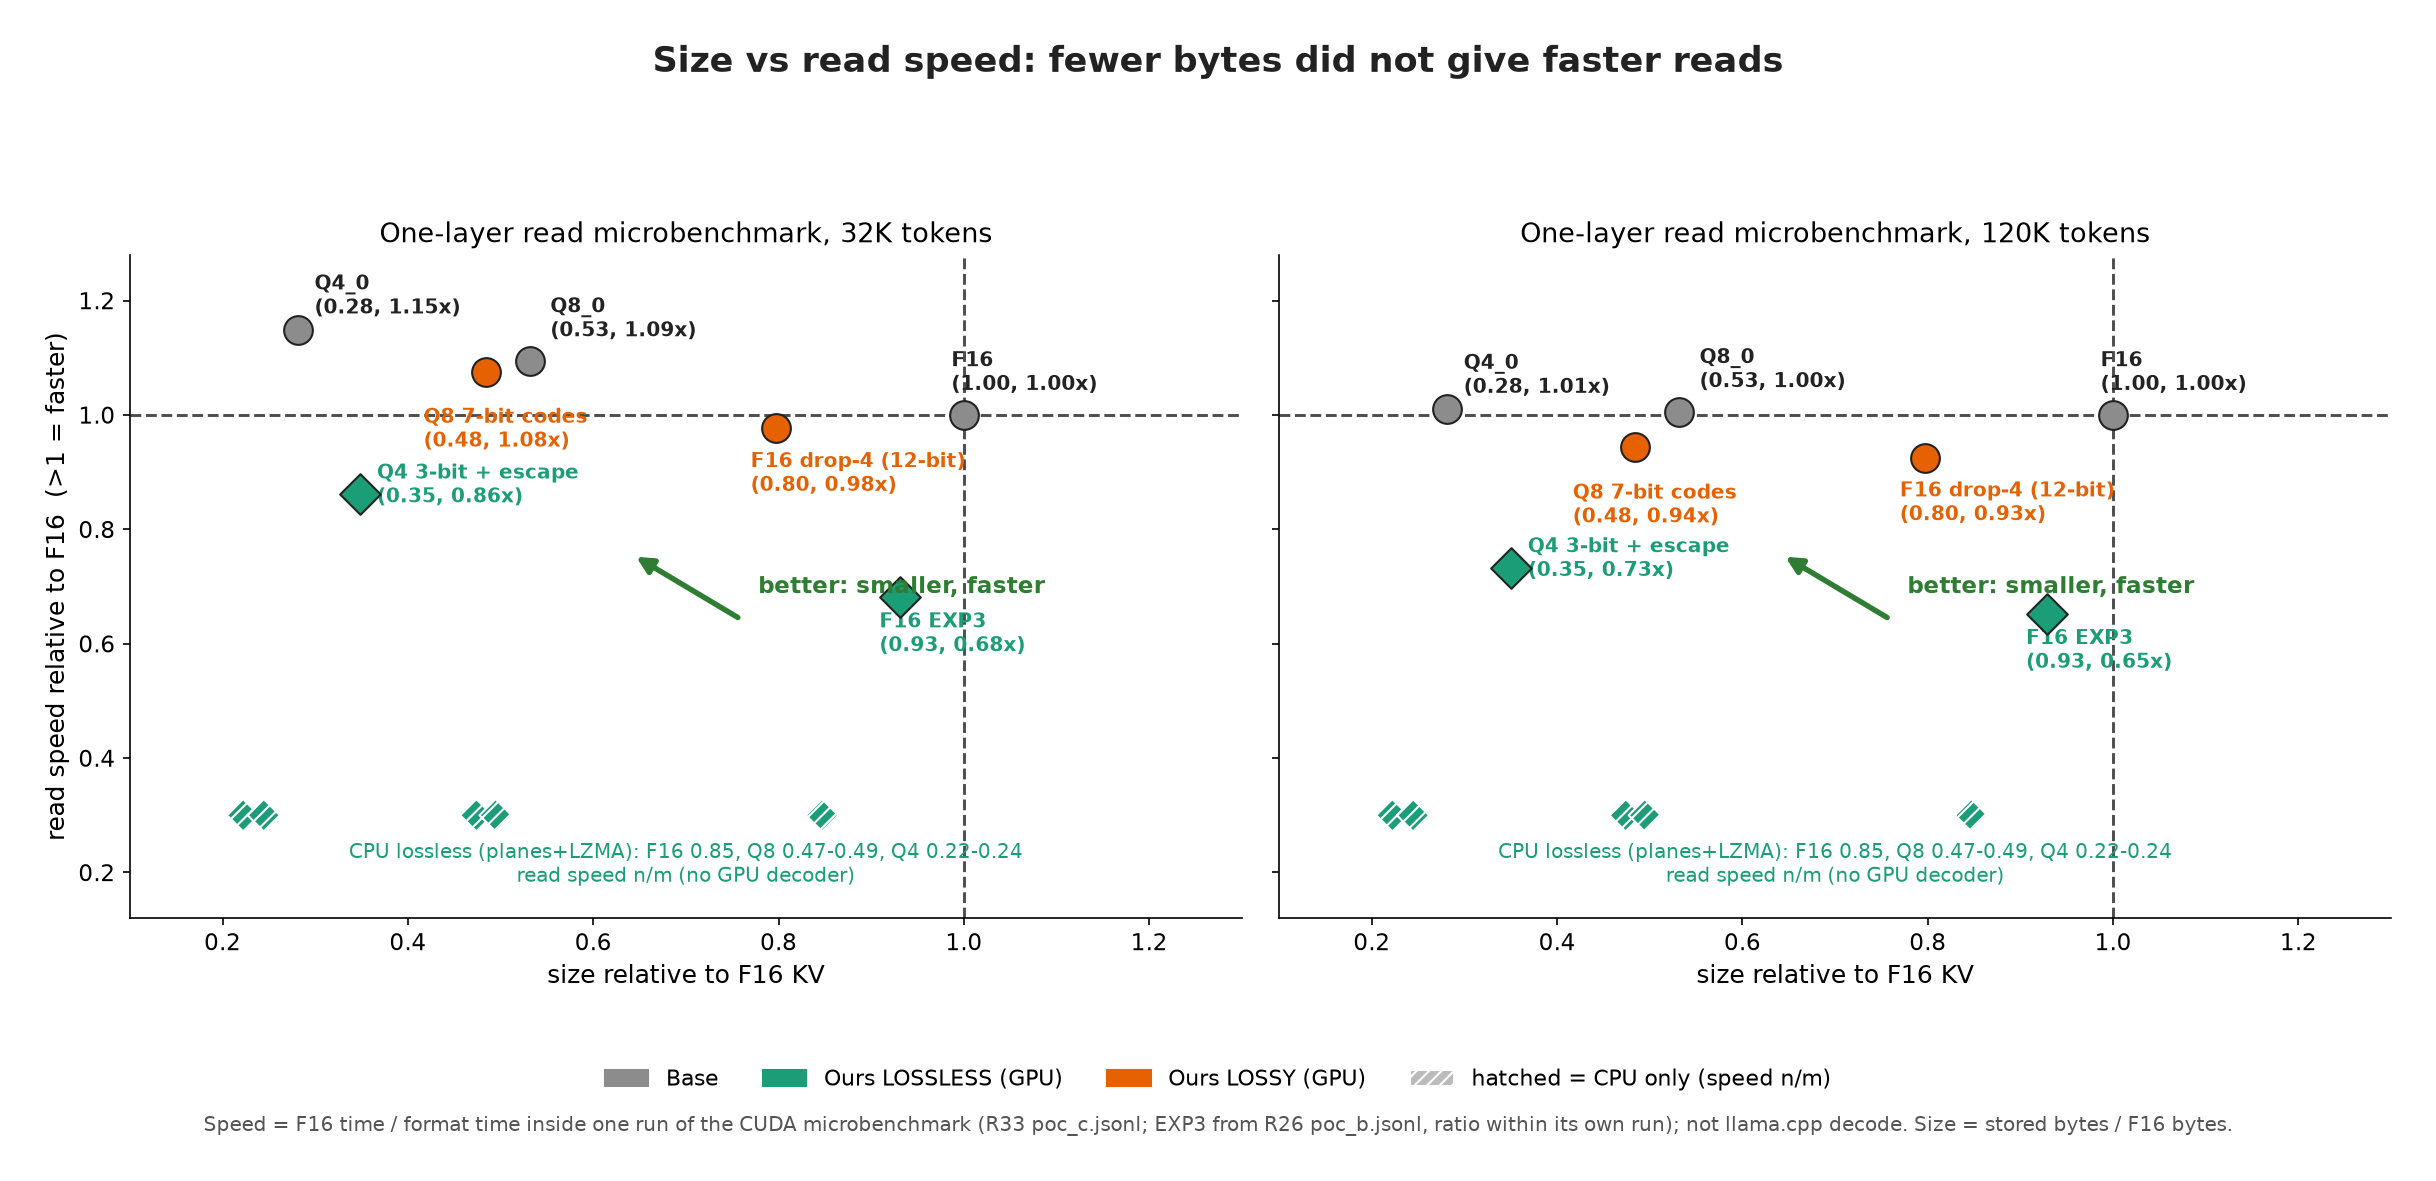
\includegraphics[width=\linewidth]{figures/fig15_pareto_size_vs_speed.png}\caption{KV size against read speed in the CUDA microbenchmark at 32K and 120K tokens. Fewer bytes did not buy faster reads (R26, R33).}\end{figure}

\begin{figure}[htbp]\centering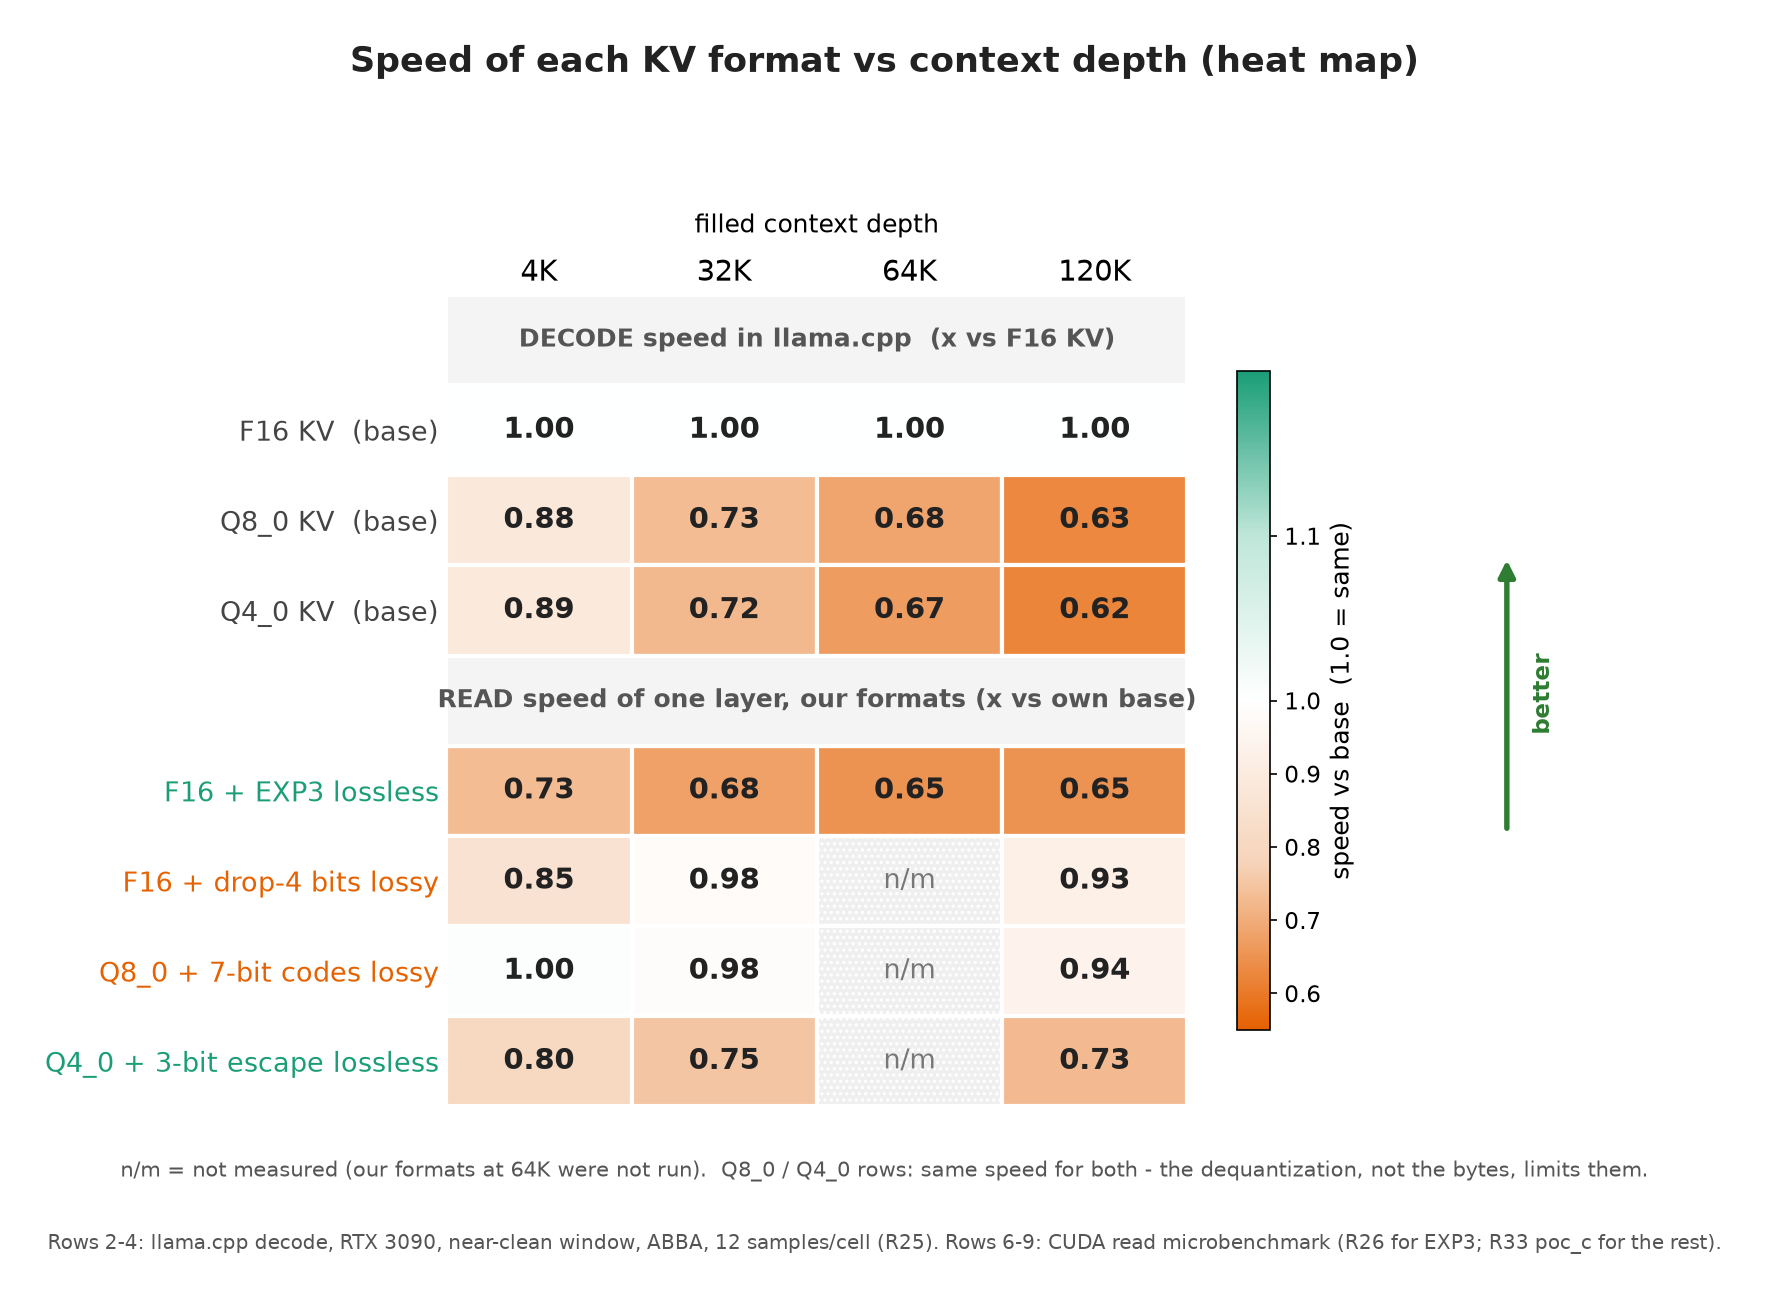
\includegraphics[width=\linewidth]{figures/fig16_heatmap_decode_speed.png}\caption{Decode speed relative to F16 KV by depth (llama.cpp, R25) and read speed of our formats relative to their own base (R26, R33).}\end{figure}

\begin{figure}[htbp]\centering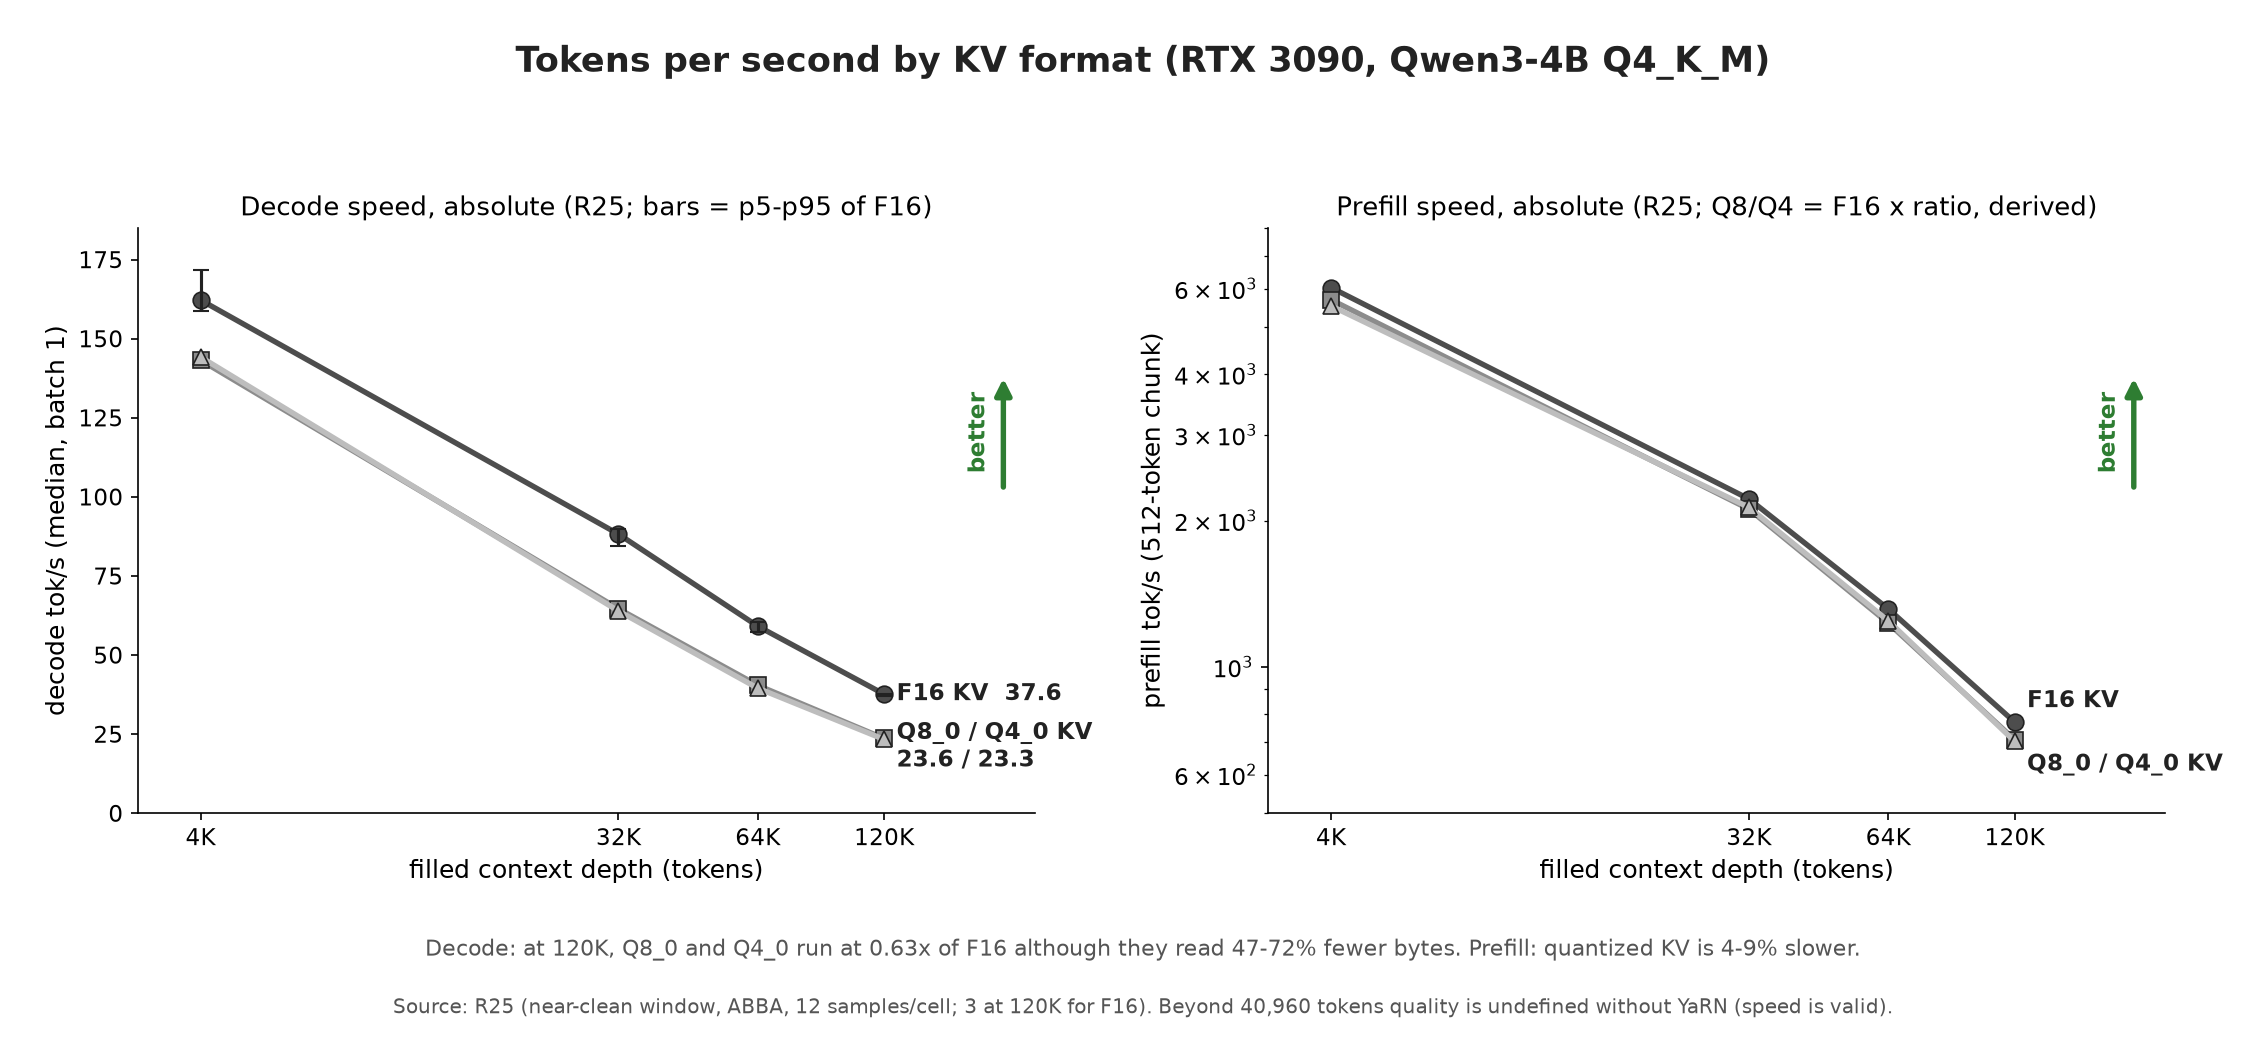
\includegraphics[width=\linewidth]{figures/fig19_absolute_toks.png}\caption{Absolute decode and prefill speed by depth (R25).}\end{figure}

\begin{figure}[htbp]\centering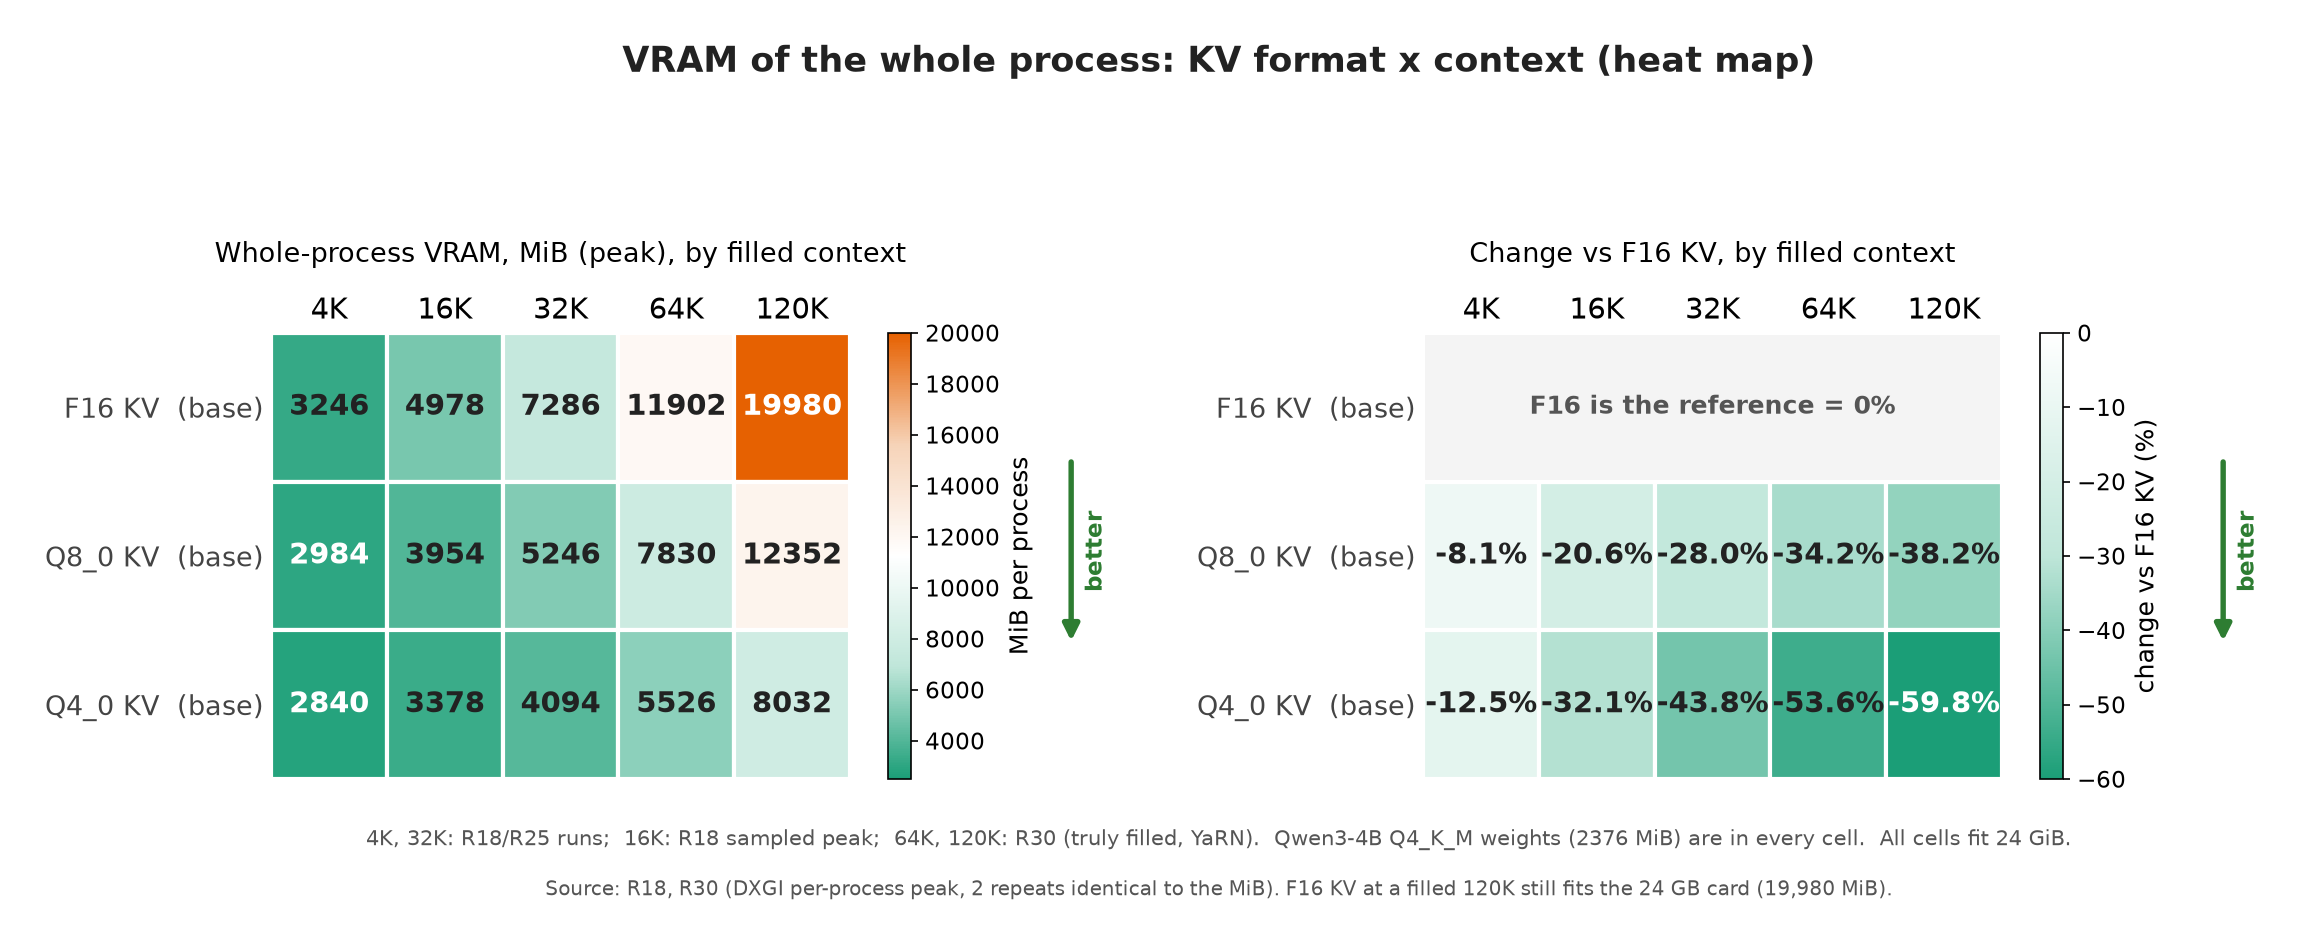
\includegraphics[width=\linewidth]{figures/fig17_heatmap_vram.png}\caption{Process VRAM by KV format and filled context (R18, R30).}\end{figure}

\begin{figure}[htbp]\centering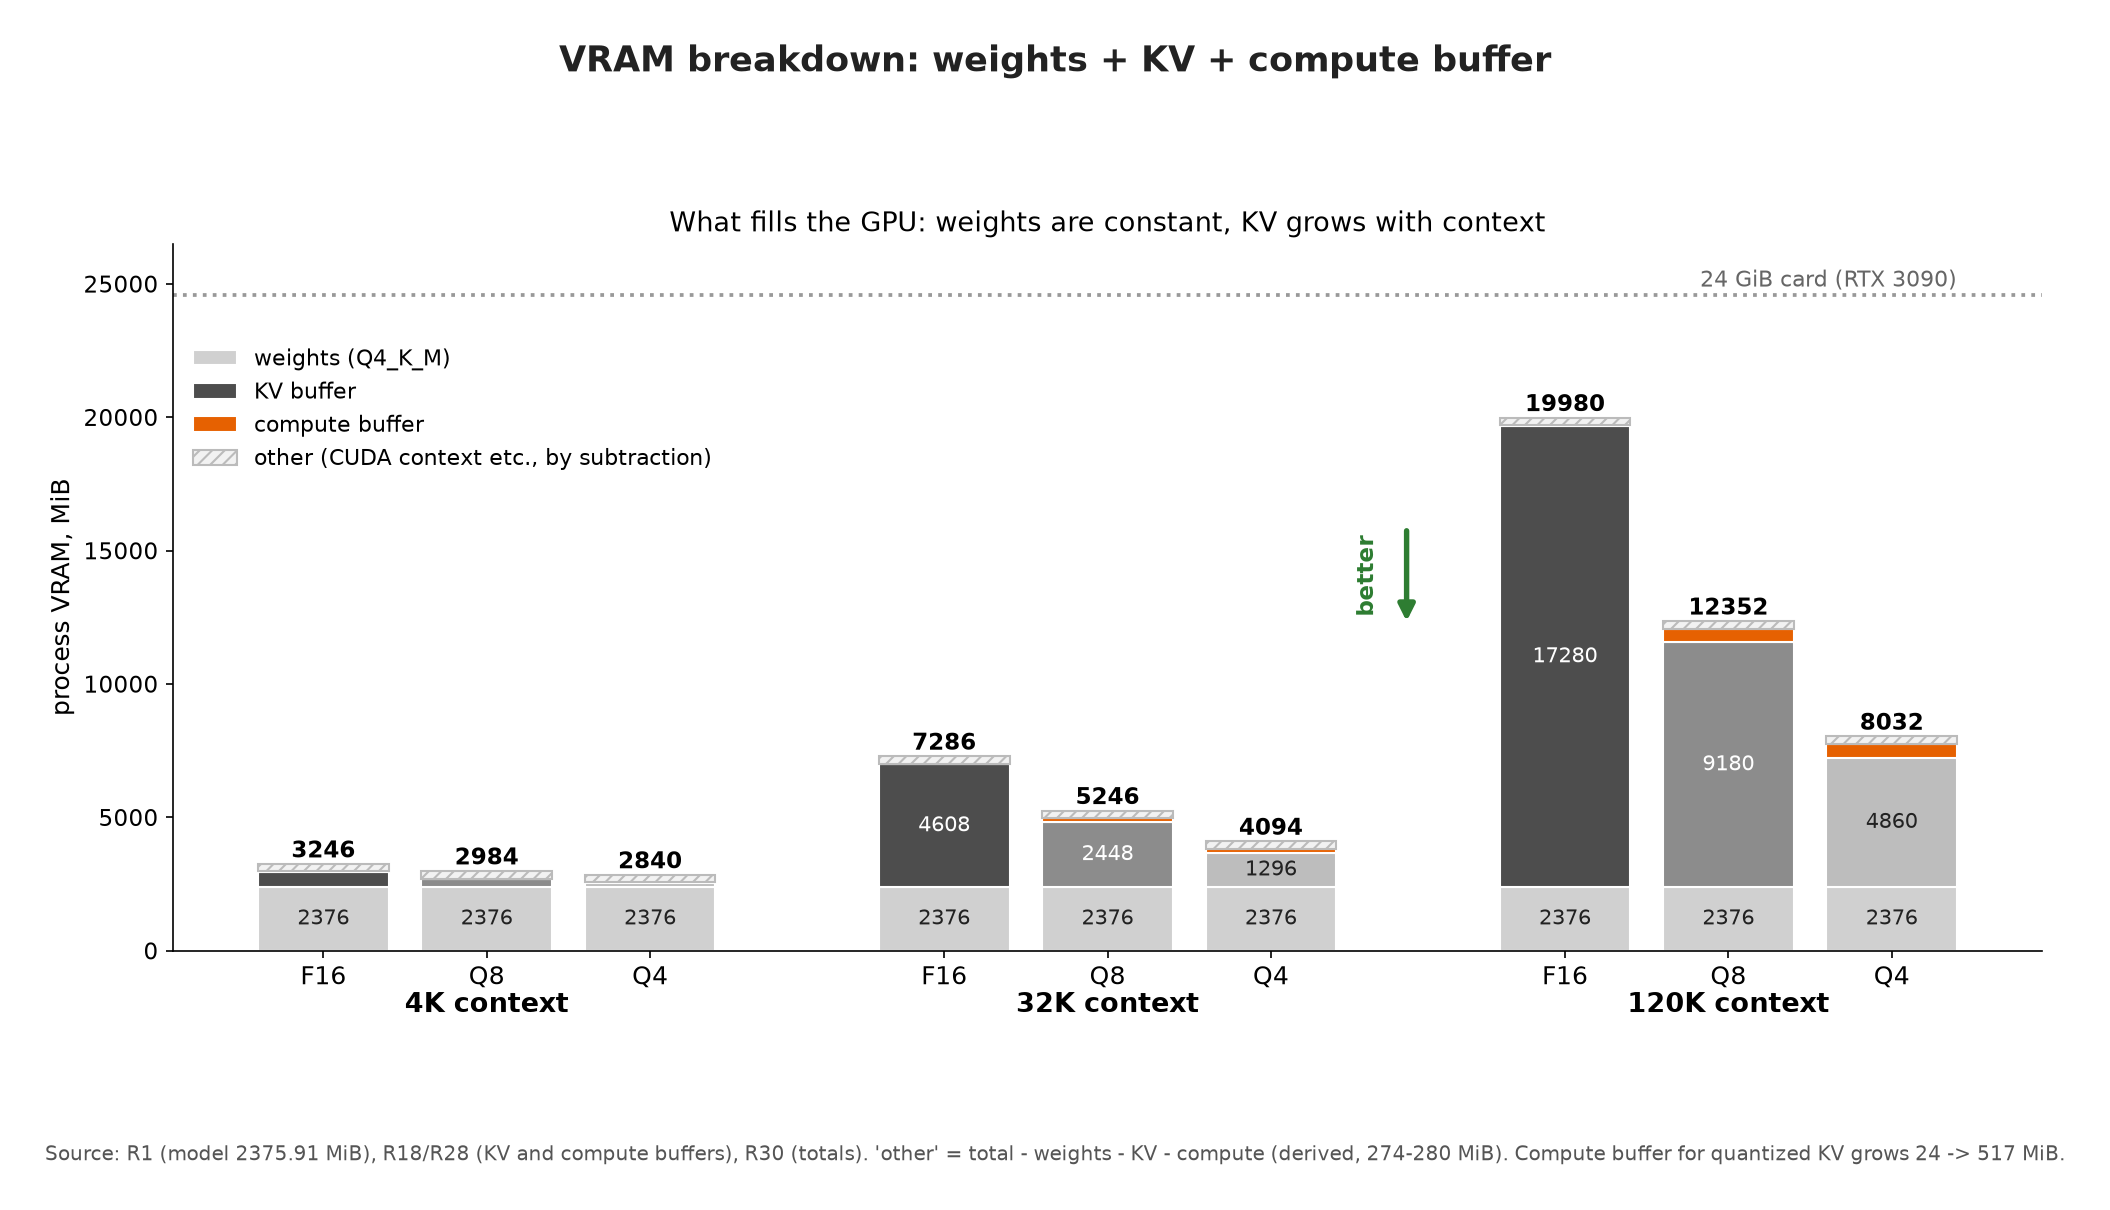
\includegraphics[width=\linewidth]{figures/fig18_vram_stacked_breakdown.png}\caption{What fills the GPU: constant weights, KV that grows with context, and a compute buffer that grows for quantized KV (R1, R18, R28, R30).}\end{figure}

\begin{figure}[htbp]\centering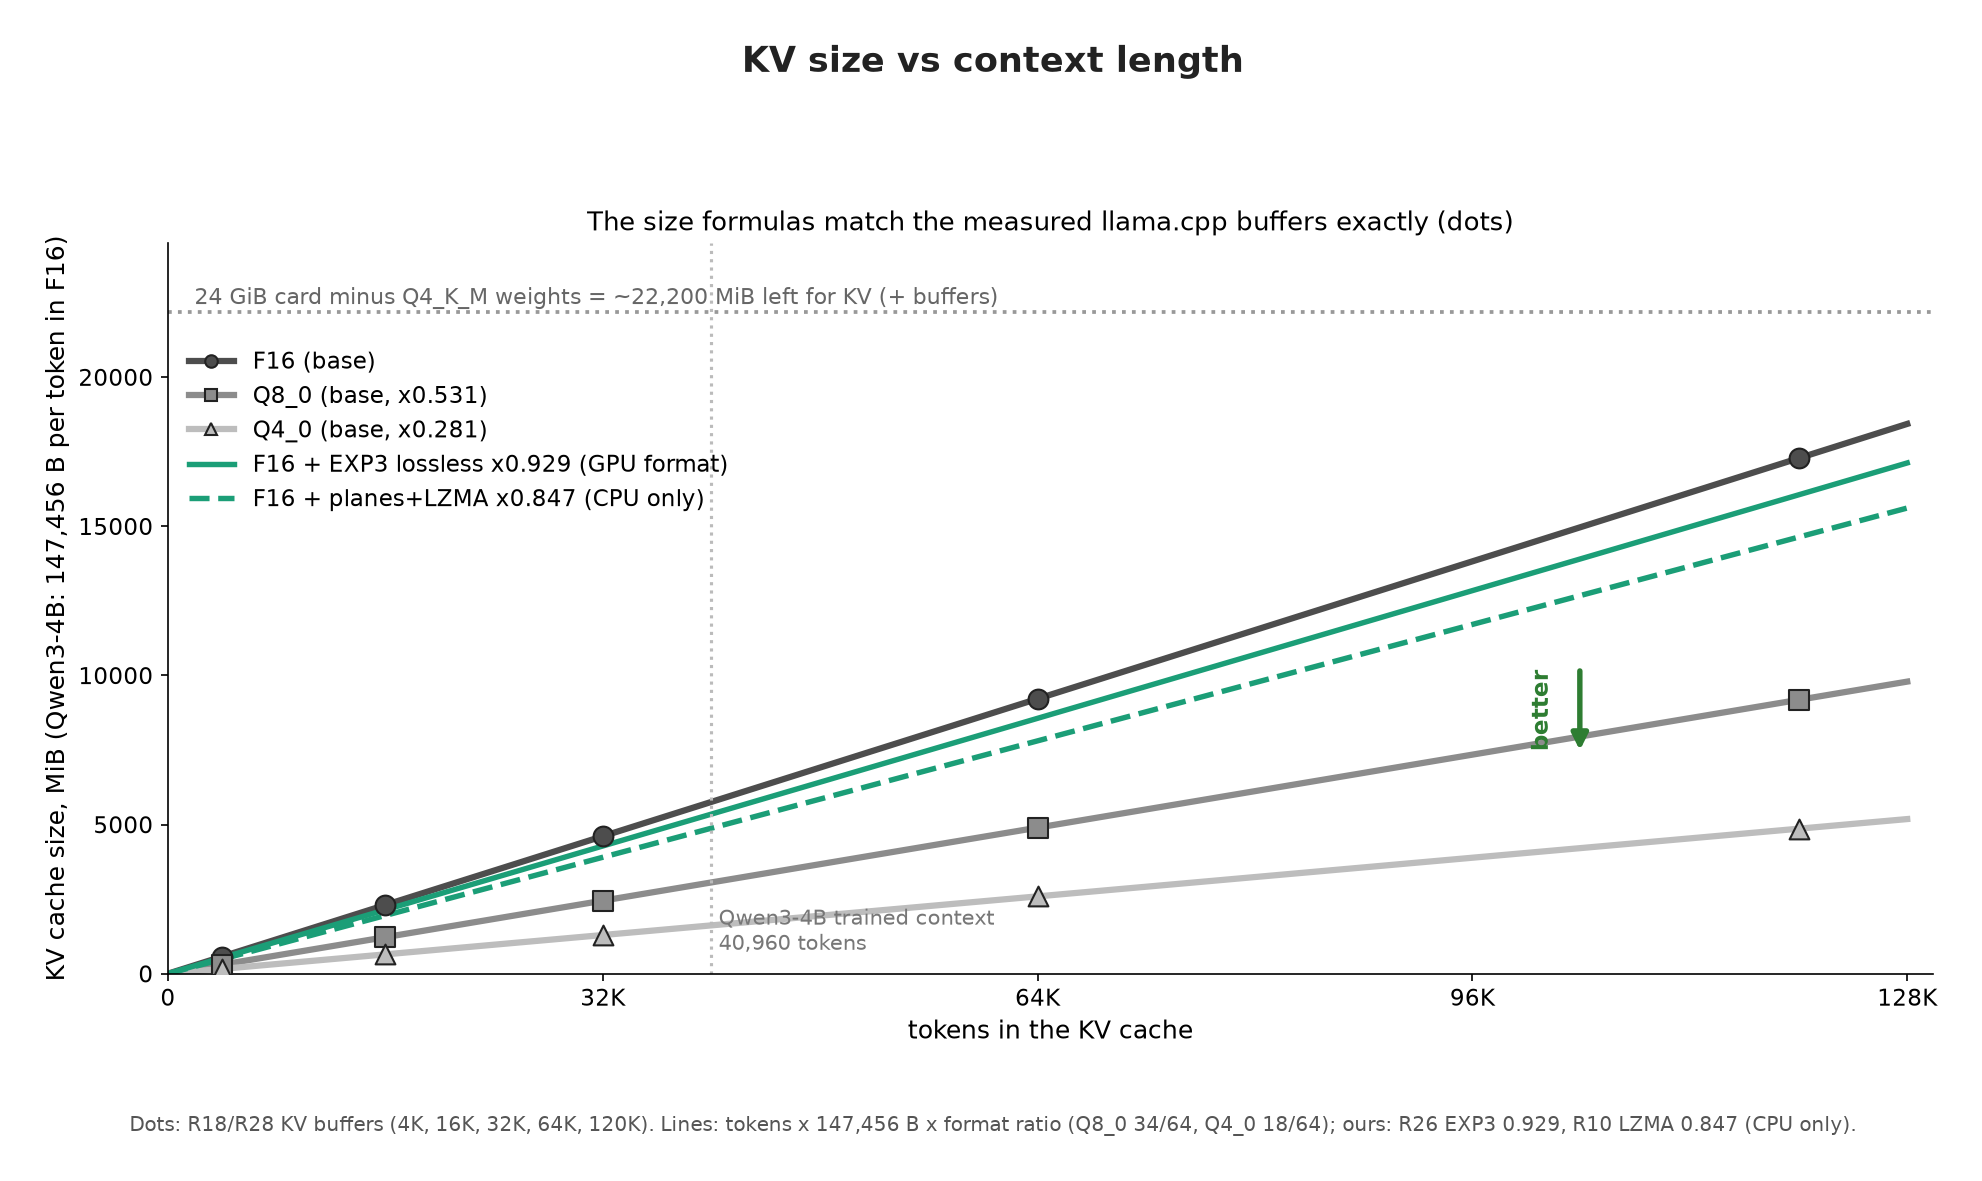
\includegraphics[width=\linewidth]{figures/fig42_kv_size_vs_context.png}\caption{KV size is linear in context length and matches llama.cpp's buffers (dots); green lines are our lossless formats (R10, R26).}\end{figure}

\begin{figure}[htbp]\centering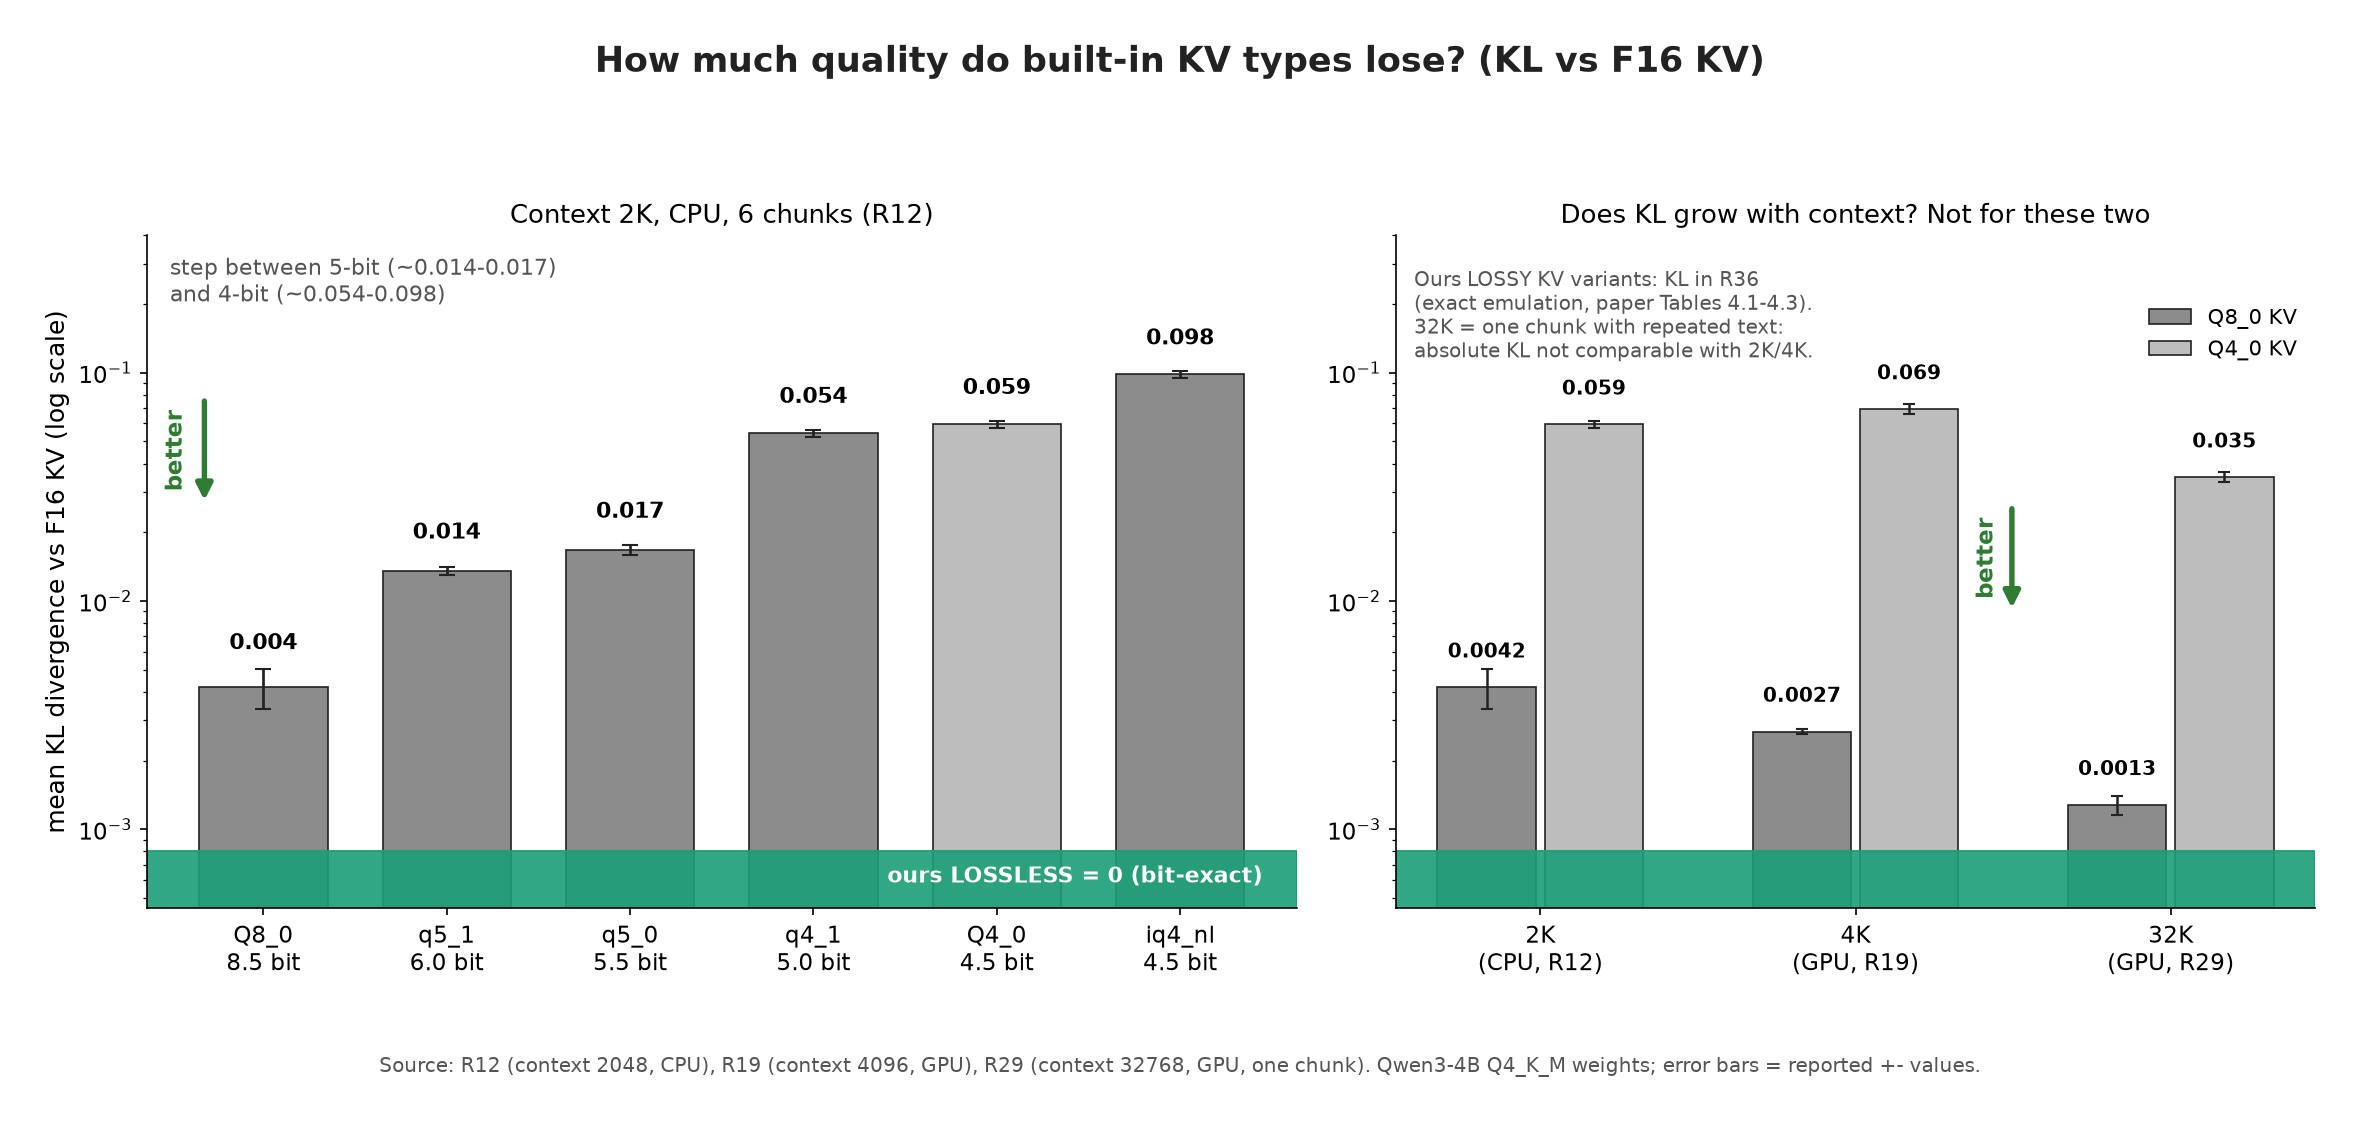
\includegraphics[width=\linewidth]{figures/fig30_kv_kl_ladder.png}\caption{KL of built-in KV types against F16 KV at 2K, 4K and 32K (R12, R19, R29). Our lossy variants: R36.}\end{figure}

\begin{figure}[htbp]\centering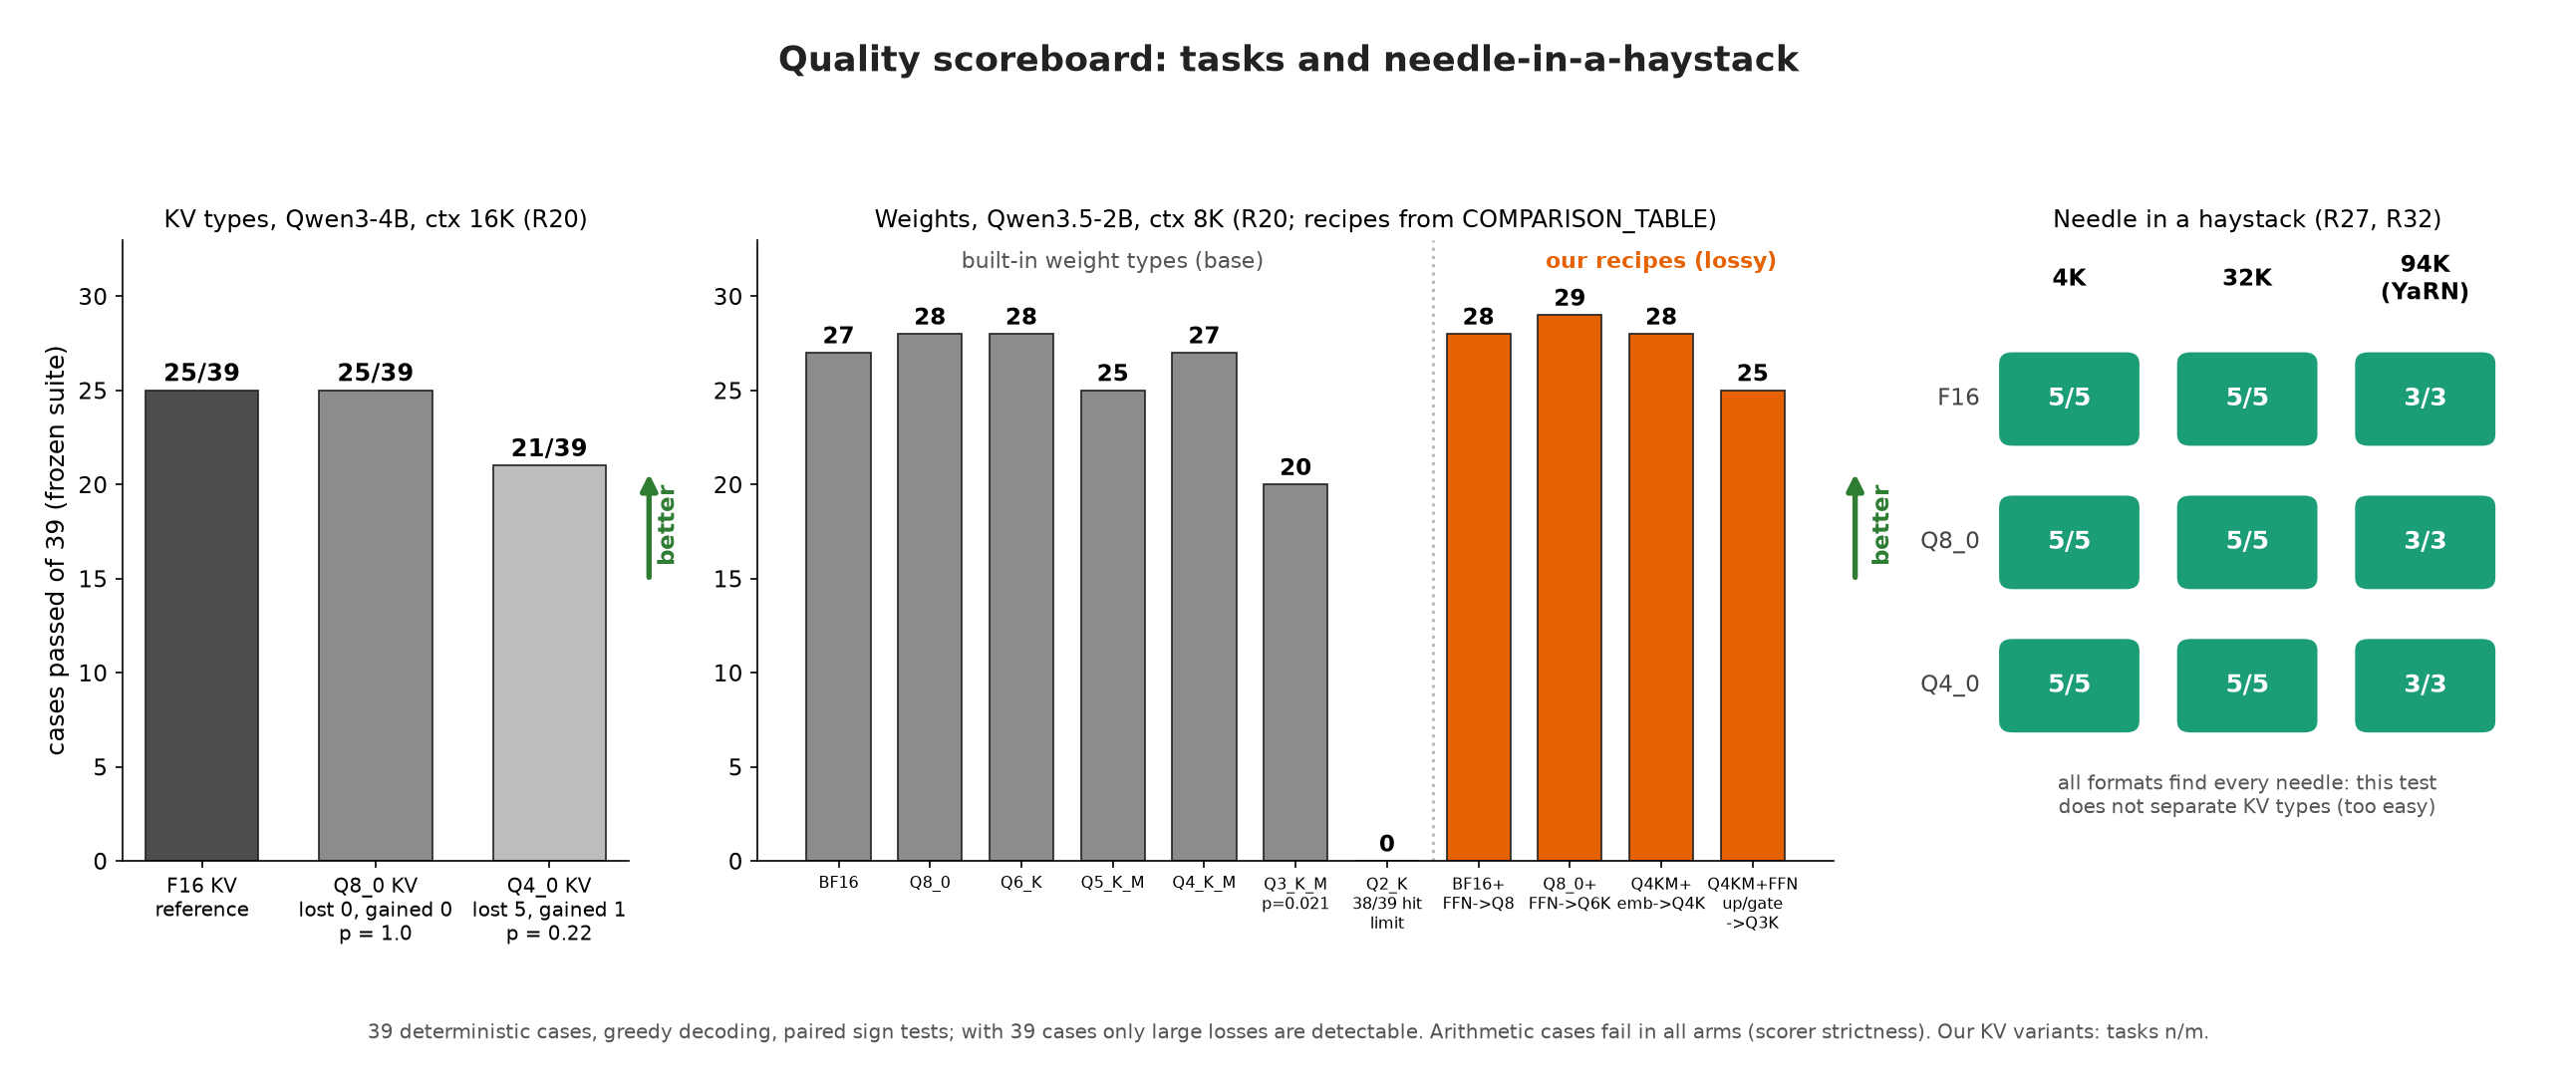
\includegraphics[width=\linewidth]{figures/fig31_quality_scoreboard.png}\caption{Tasks passed on the frozen 39-case suite and needle-in-a-haystack results (R20, R27, R32). With 39 cases only large losses are detectable.}\end{figure}

\begin{figure}[htbp]\centering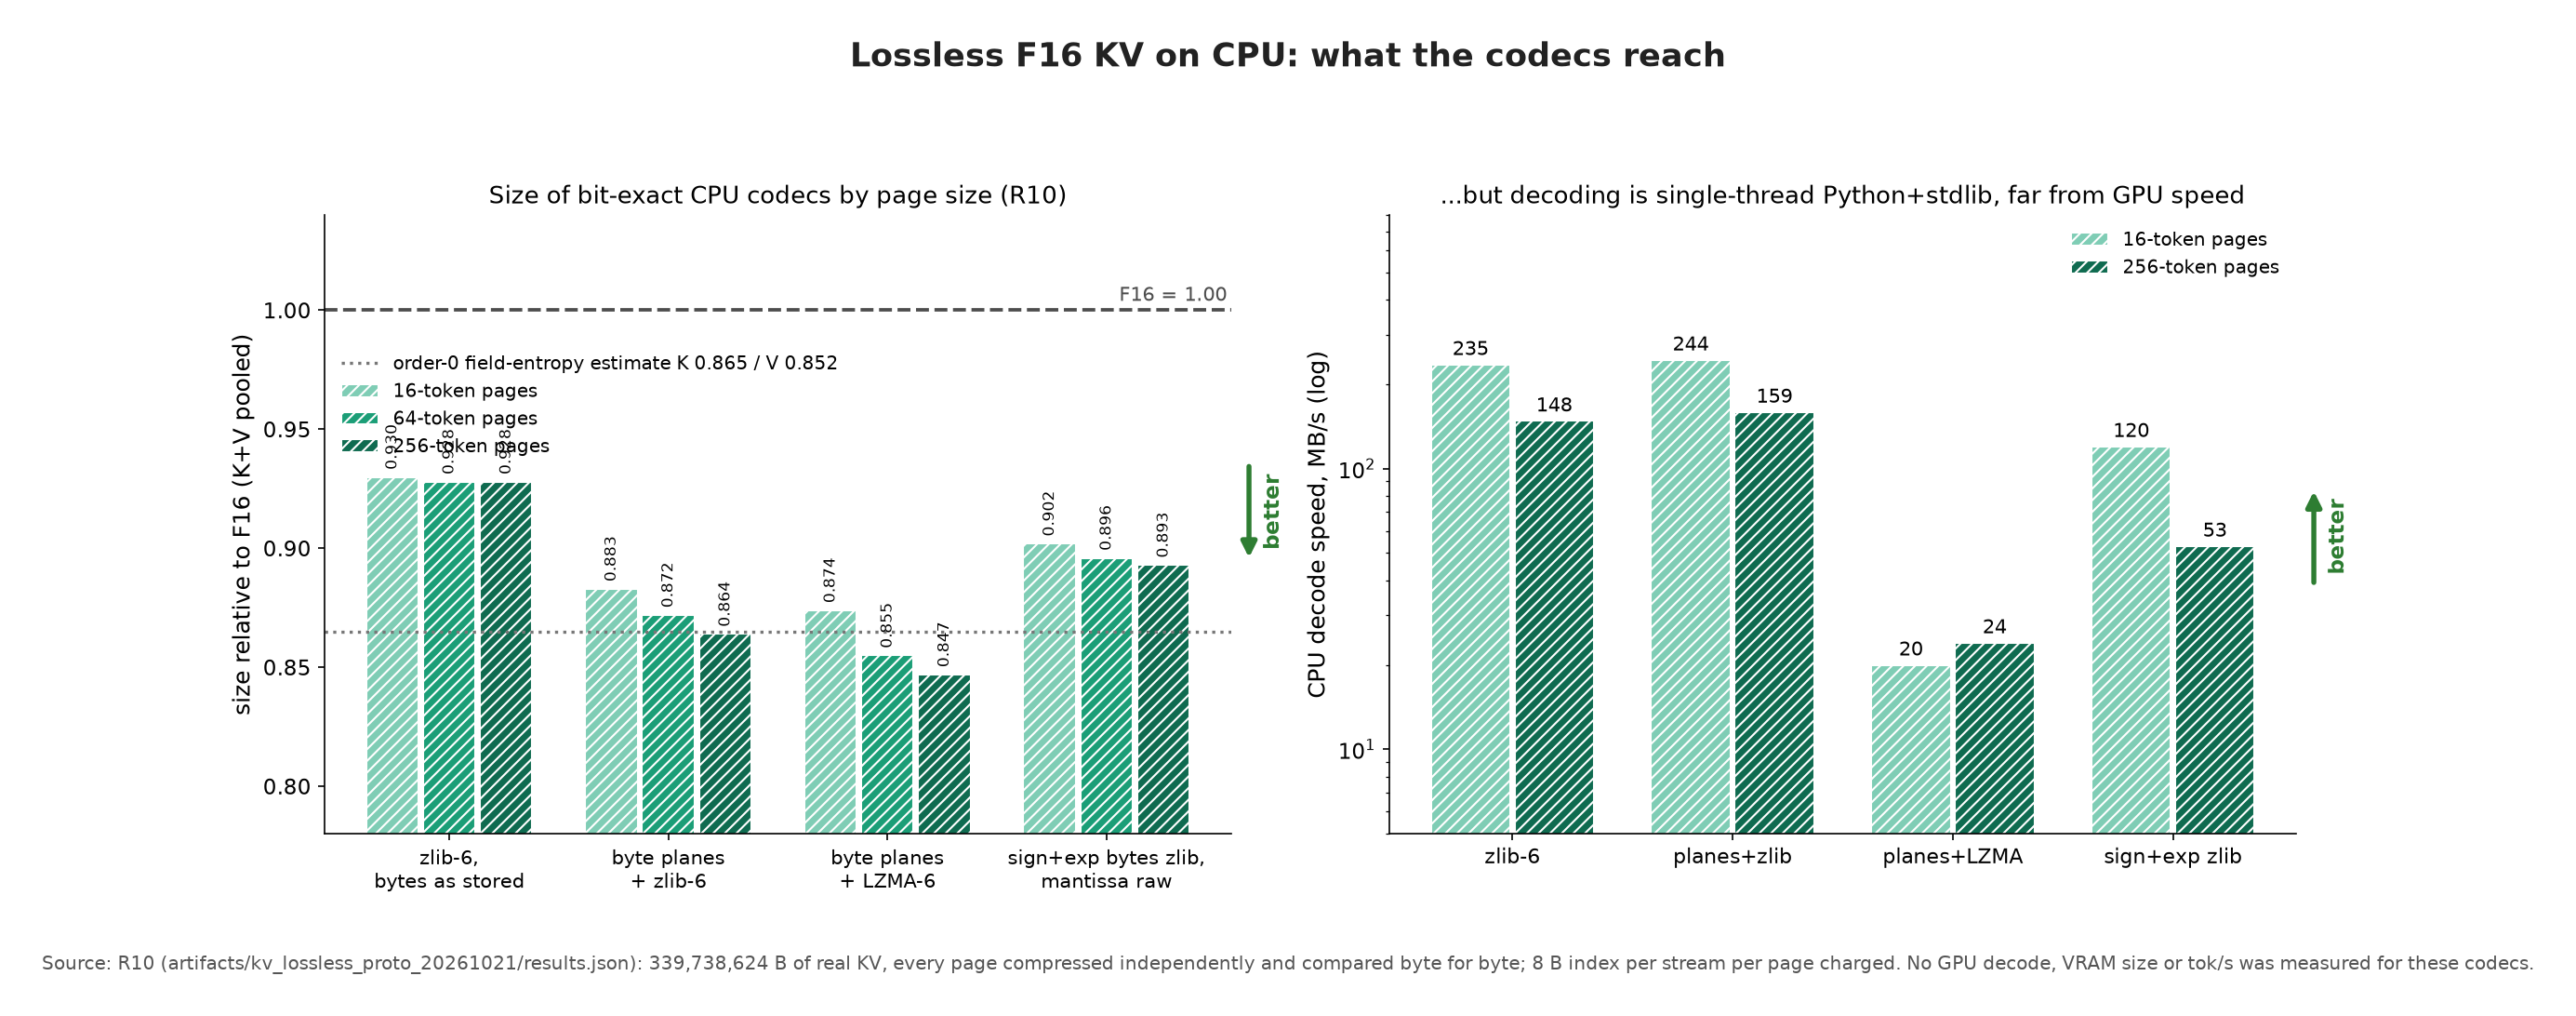
\includegraphics[width=\linewidth]{figures/fig32_lossless_f16_codecs_pages.png}\caption{Bit-exact CPU codecs on F16 KV by page size, with their CPU decode speed (R10).}\end{figure}

\begin{figure}[htbp]\centering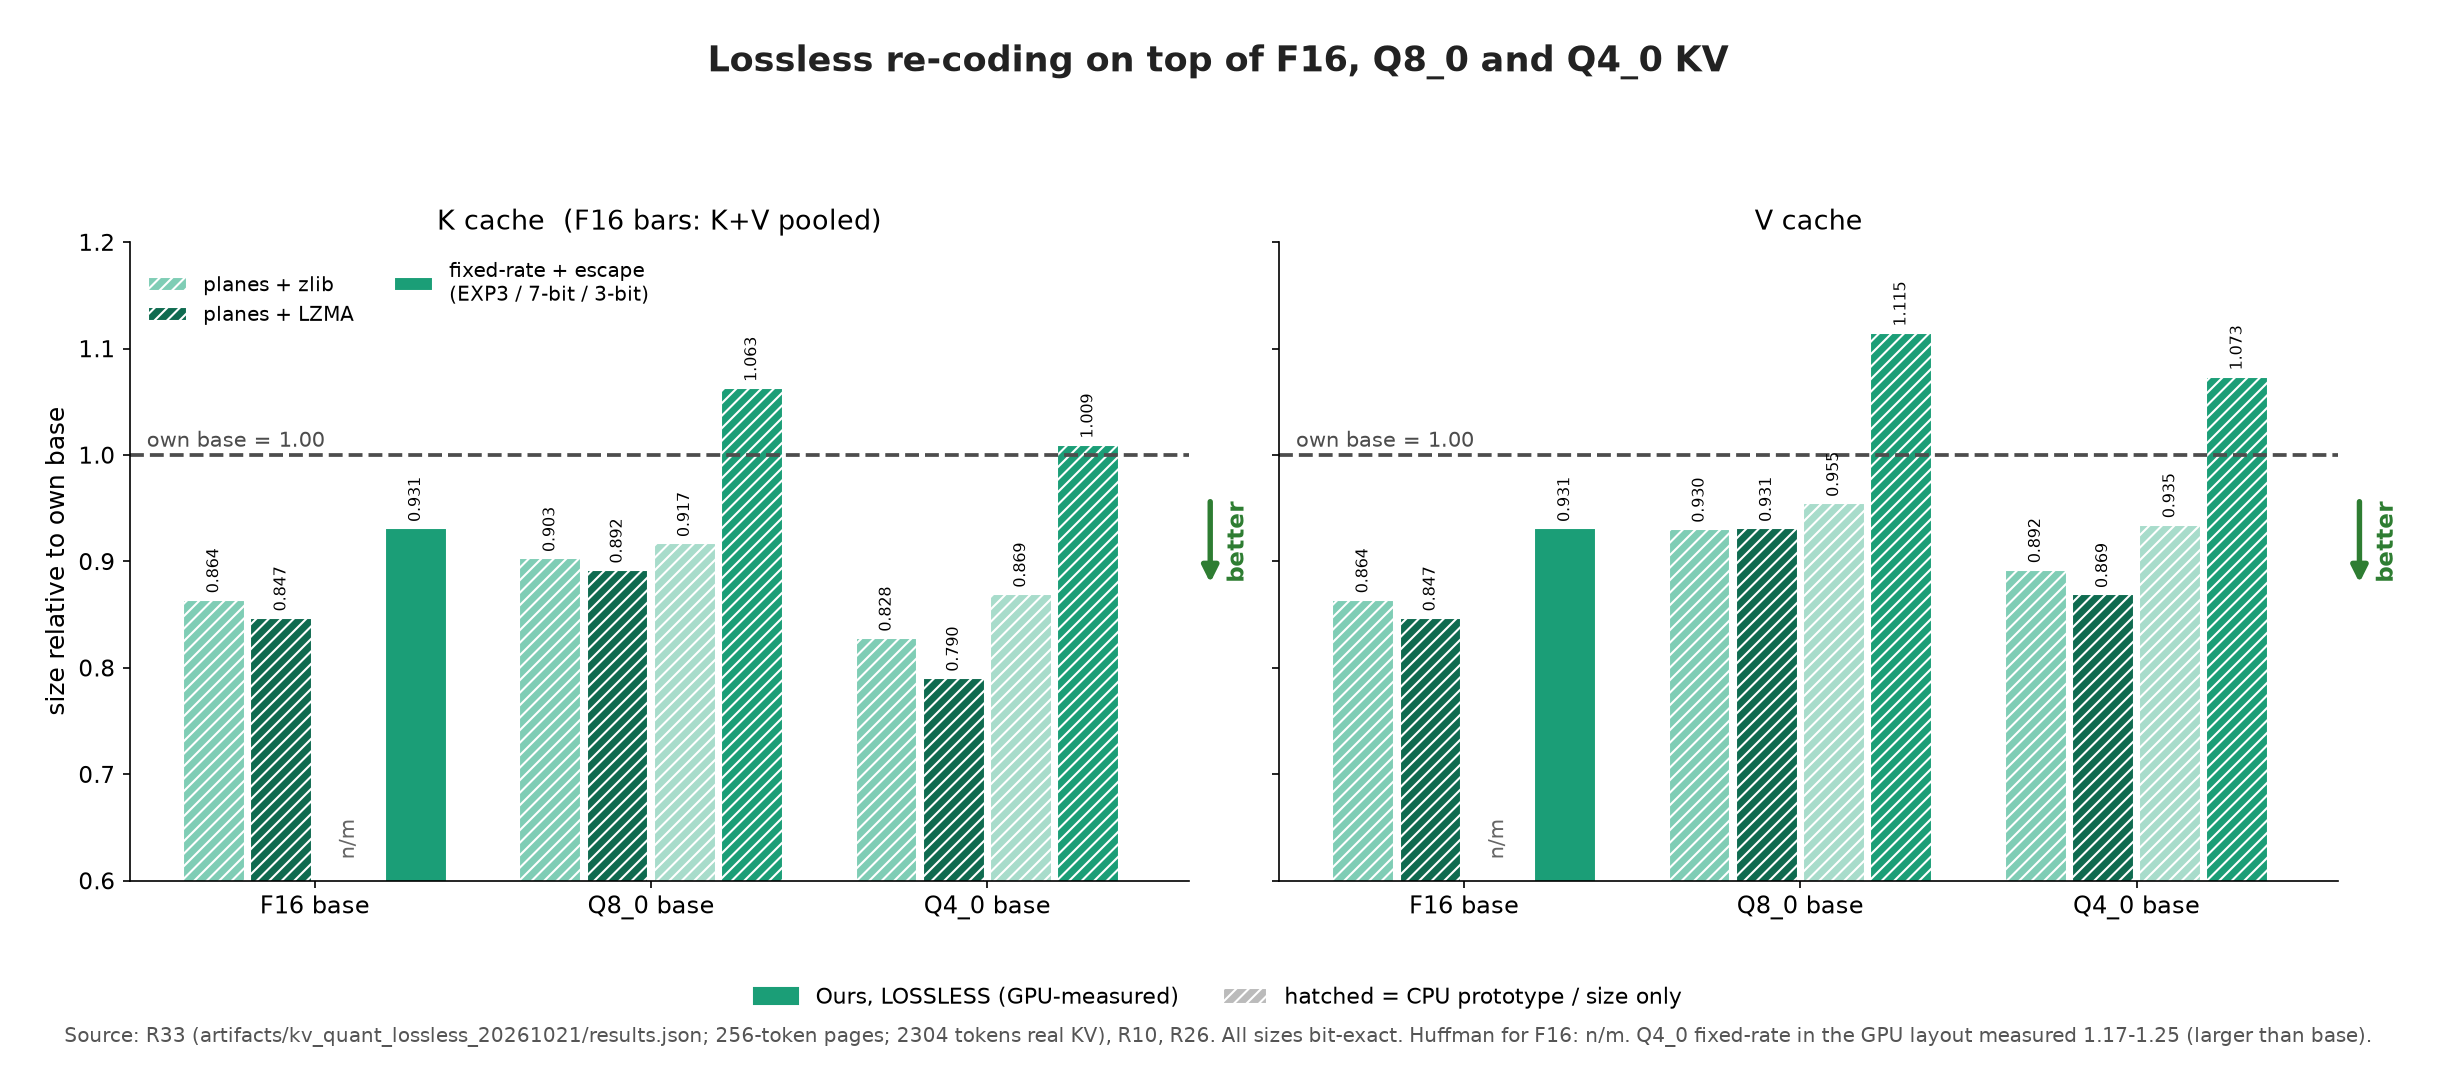
\includegraphics[width=\linewidth]{figures/fig33_lossless_on_three_bases.png}\caption{Lossless re-coding on top of F16, Q8\_0 and Q4\_0 KV; the fixed-rate variants are larger than the quantized bases (R33).}\end{figure}

\begin{figure}[htbp]\centering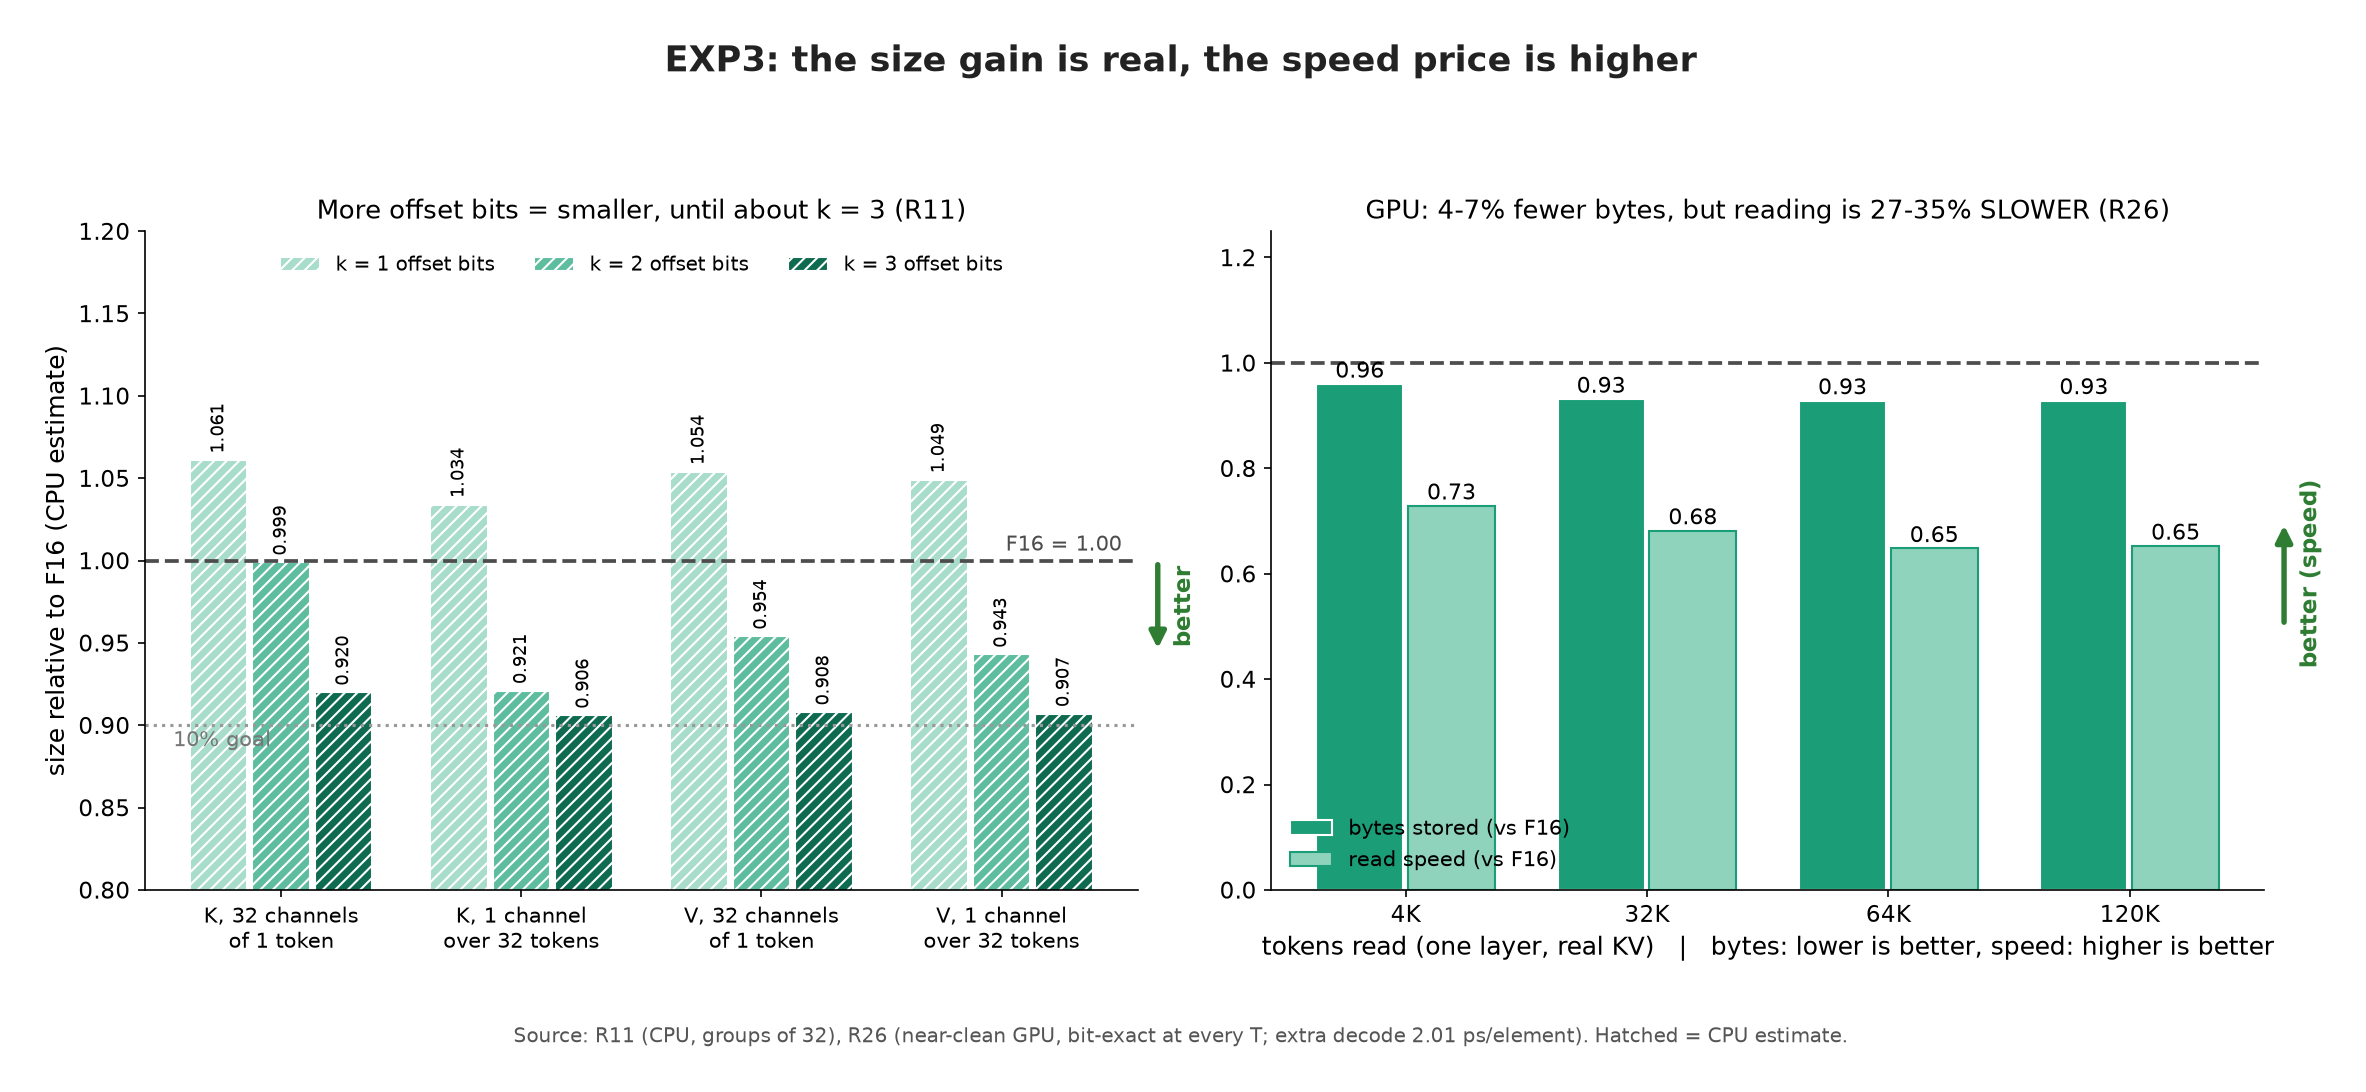
\includegraphics[width=\linewidth]{figures/fig34_exp3_ksweep_and_gpu_cost.png}\caption{EXP3: size by number of offset bits (CPU) and what it costs on the GPU: 4--7\% fewer bytes, 27--35\% slower reads (R11, R26).}\end{figure}

\begin{figure}[htbp]\centering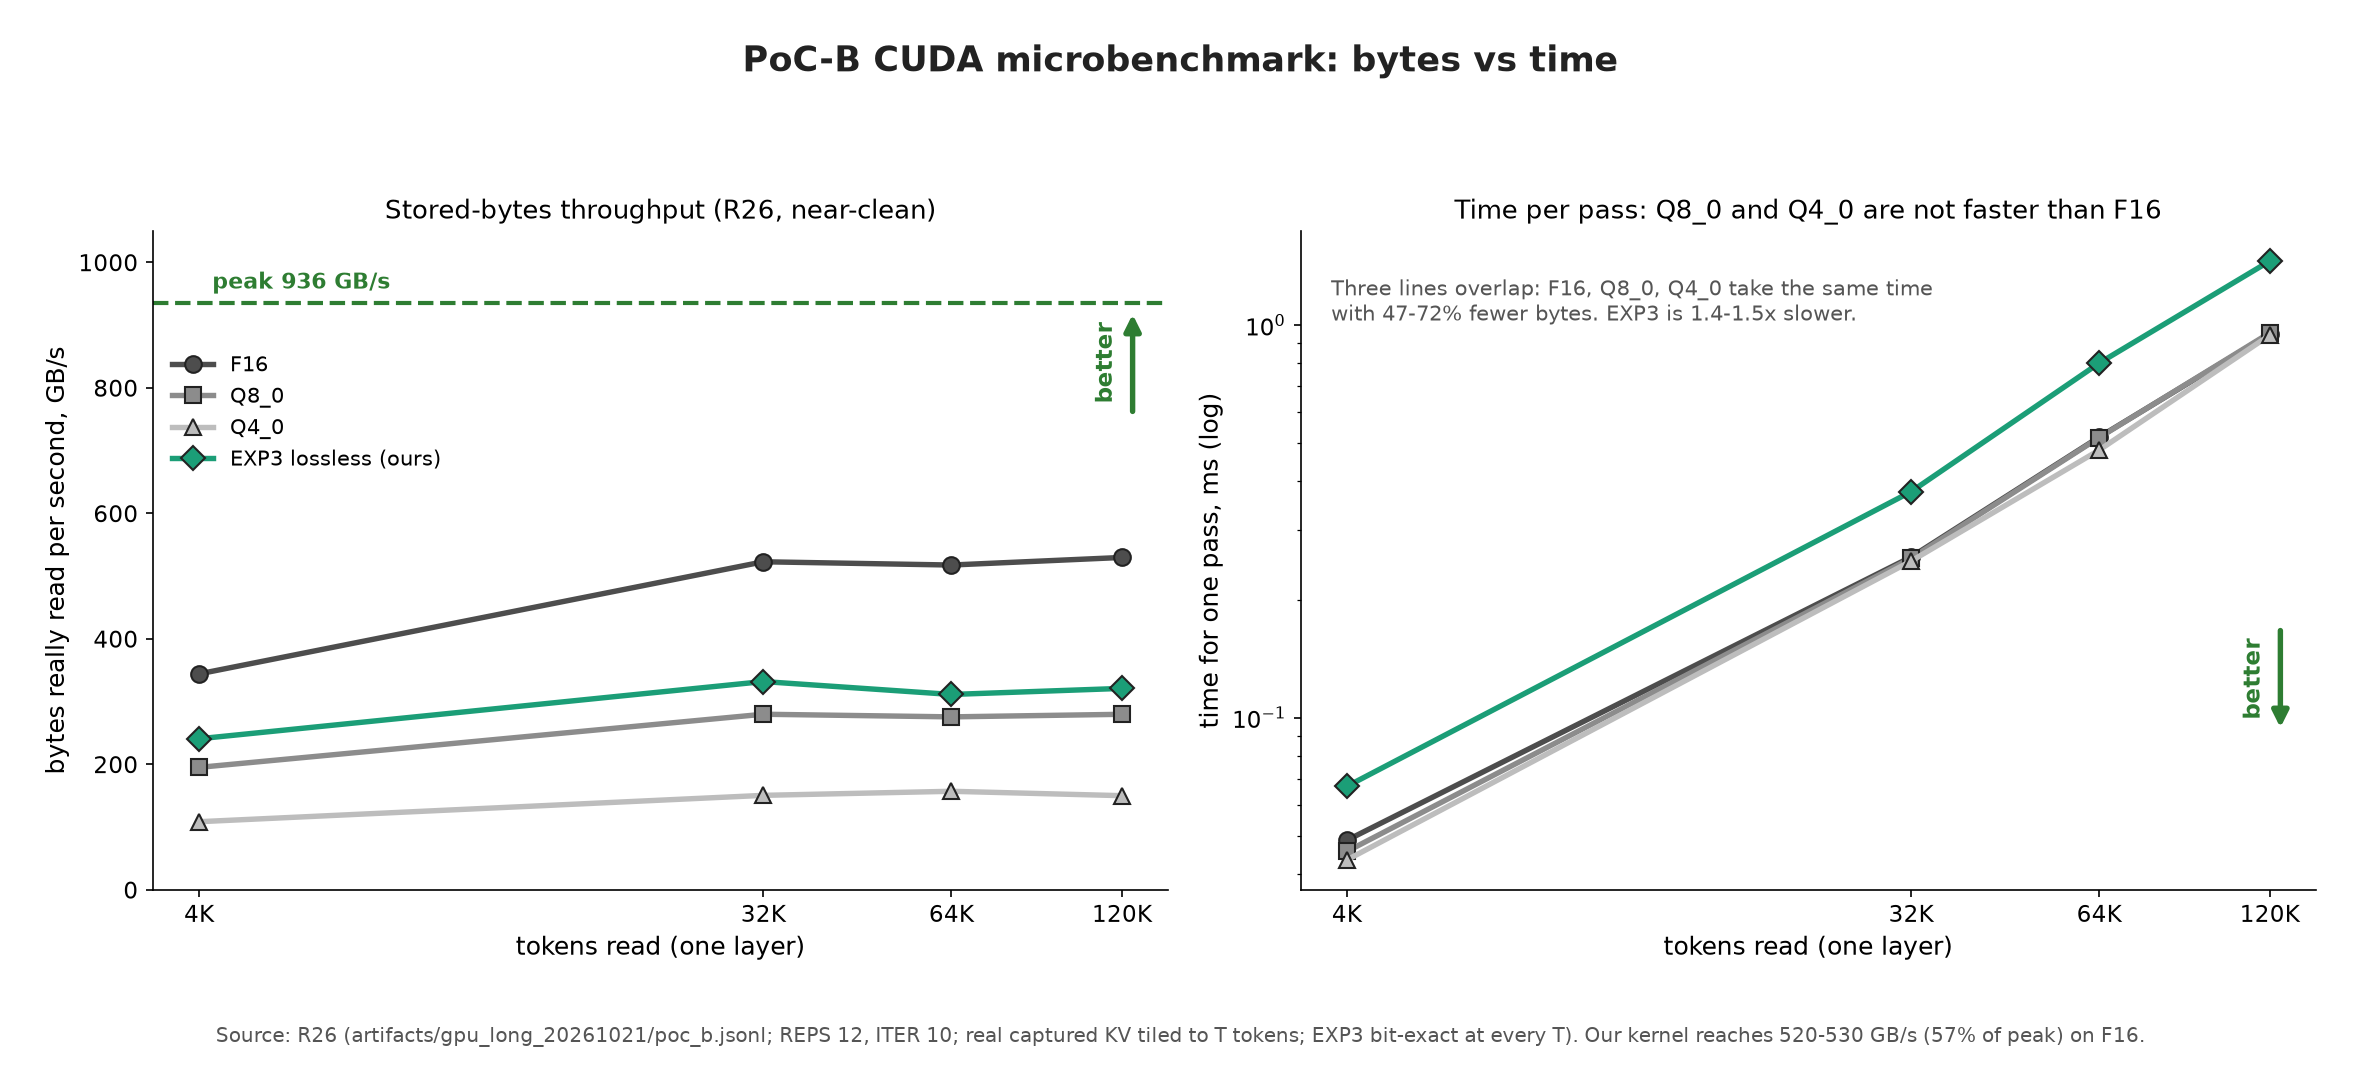
\includegraphics[width=\linewidth]{figures/fig41_pocb_throughput_and_time.png}\caption{PoC-B: throughput of stored bytes and time per pass by context (R26).}\end{figure}

\begin{figure}[htbp]\centering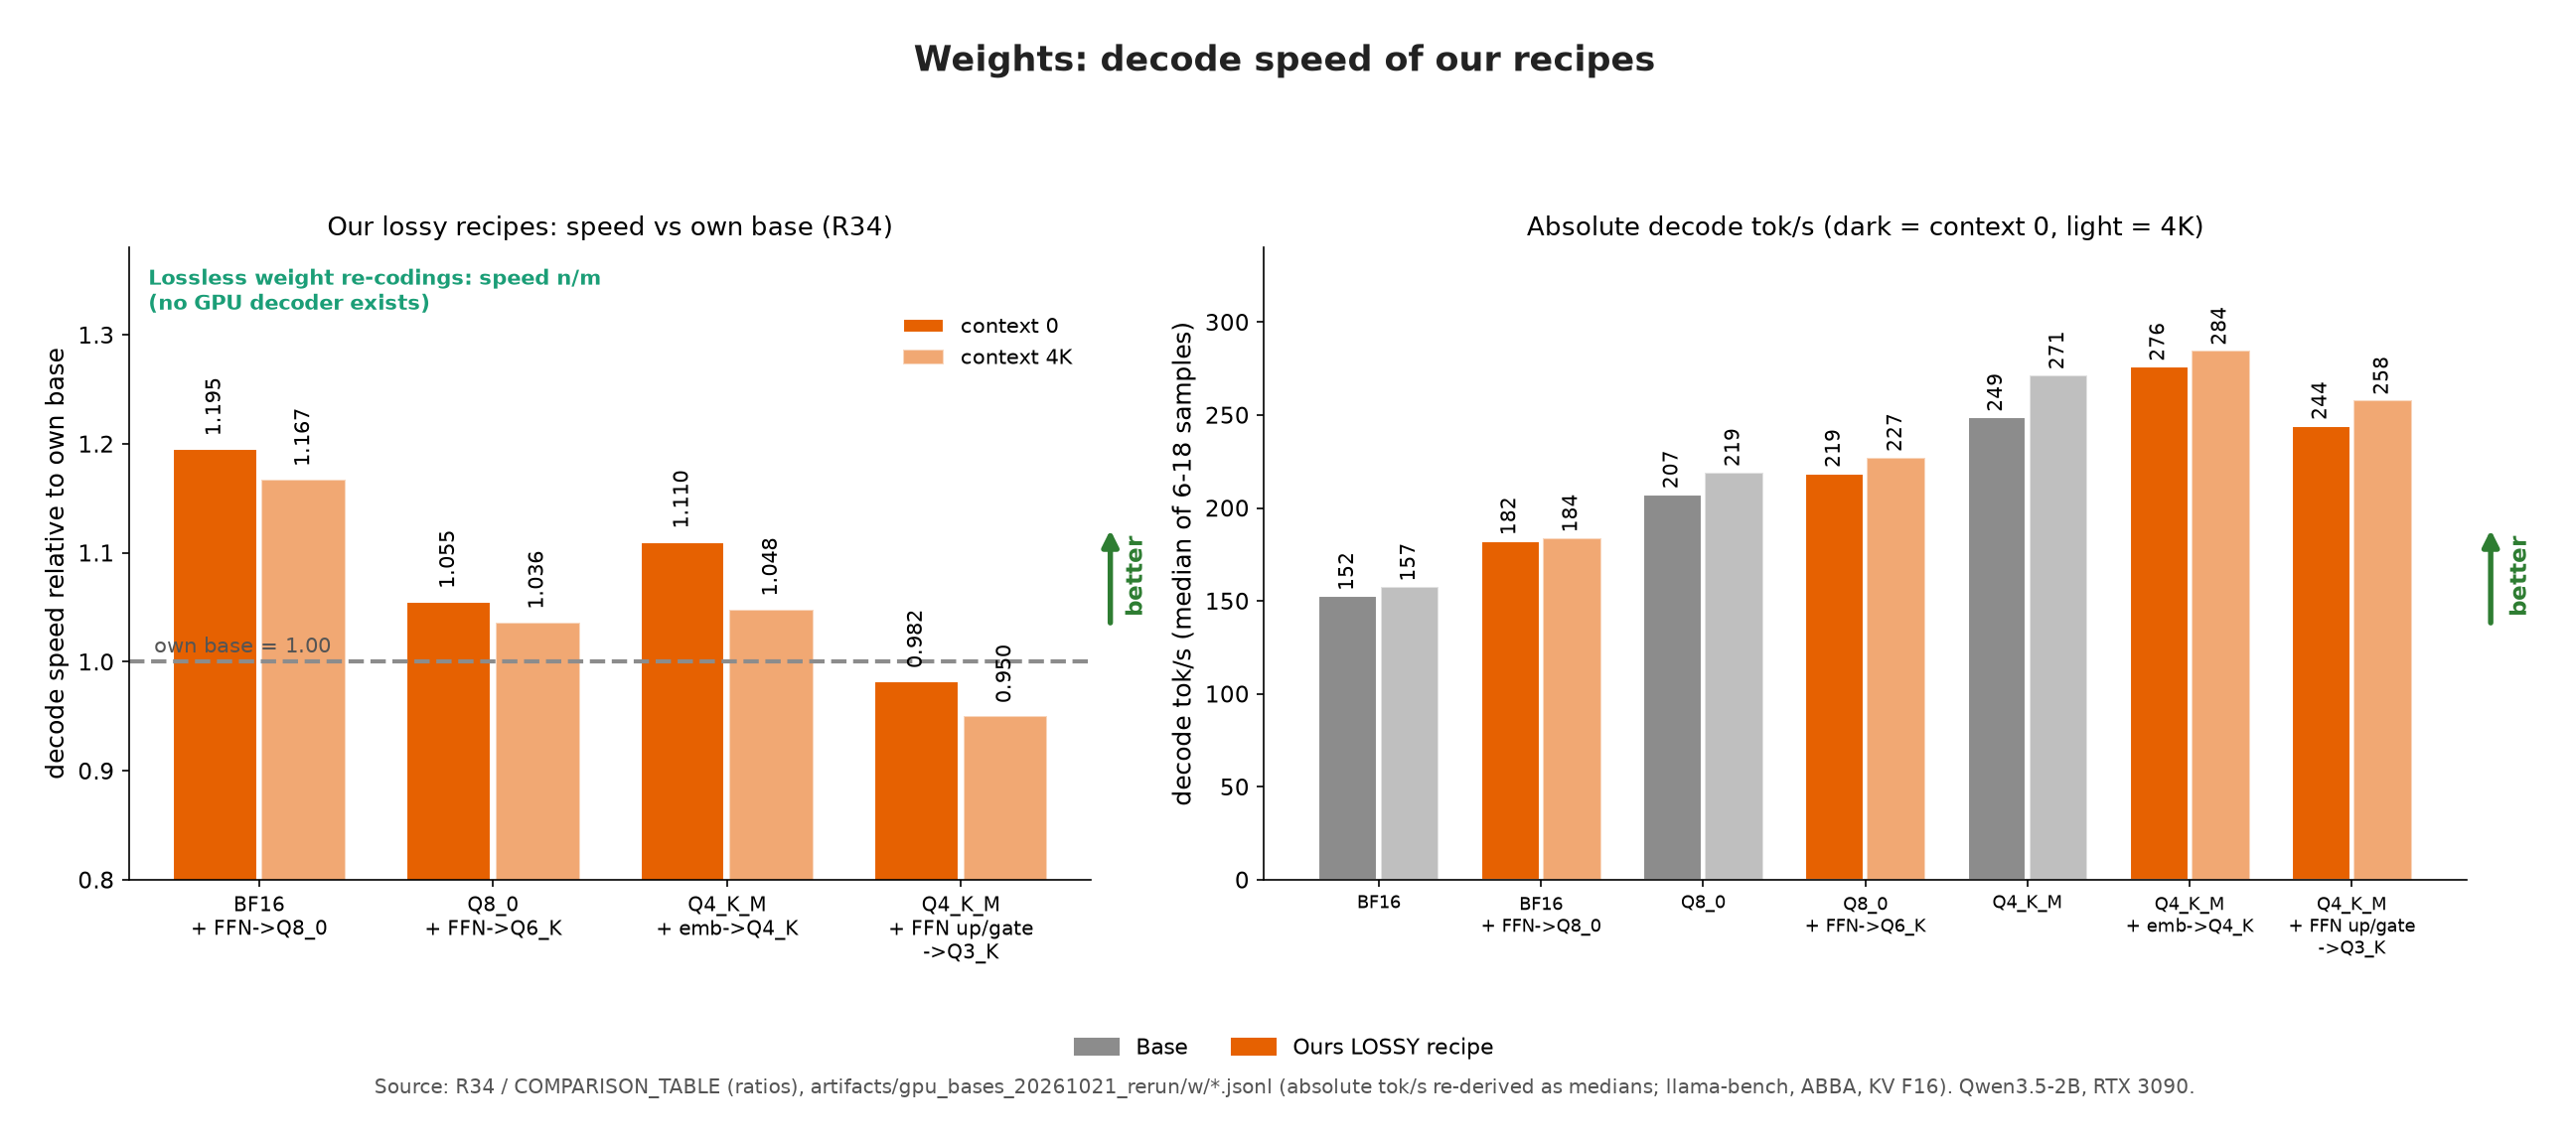
\includegraphics[width=\linewidth]{figures/fig25_weights_recipe_speed.png}\caption{Decode speed of the weight recipes relative to their base in the near-clean run (R34: +17--20\% for BF16 + FFN Q8\_0). The clean rerun gives 1.16--1.18$\times$, 1.04--1.06$\times$ and 1.02--1.05$\times$ (R37).}\end{figure}

\begin{figure}[htbp]\centering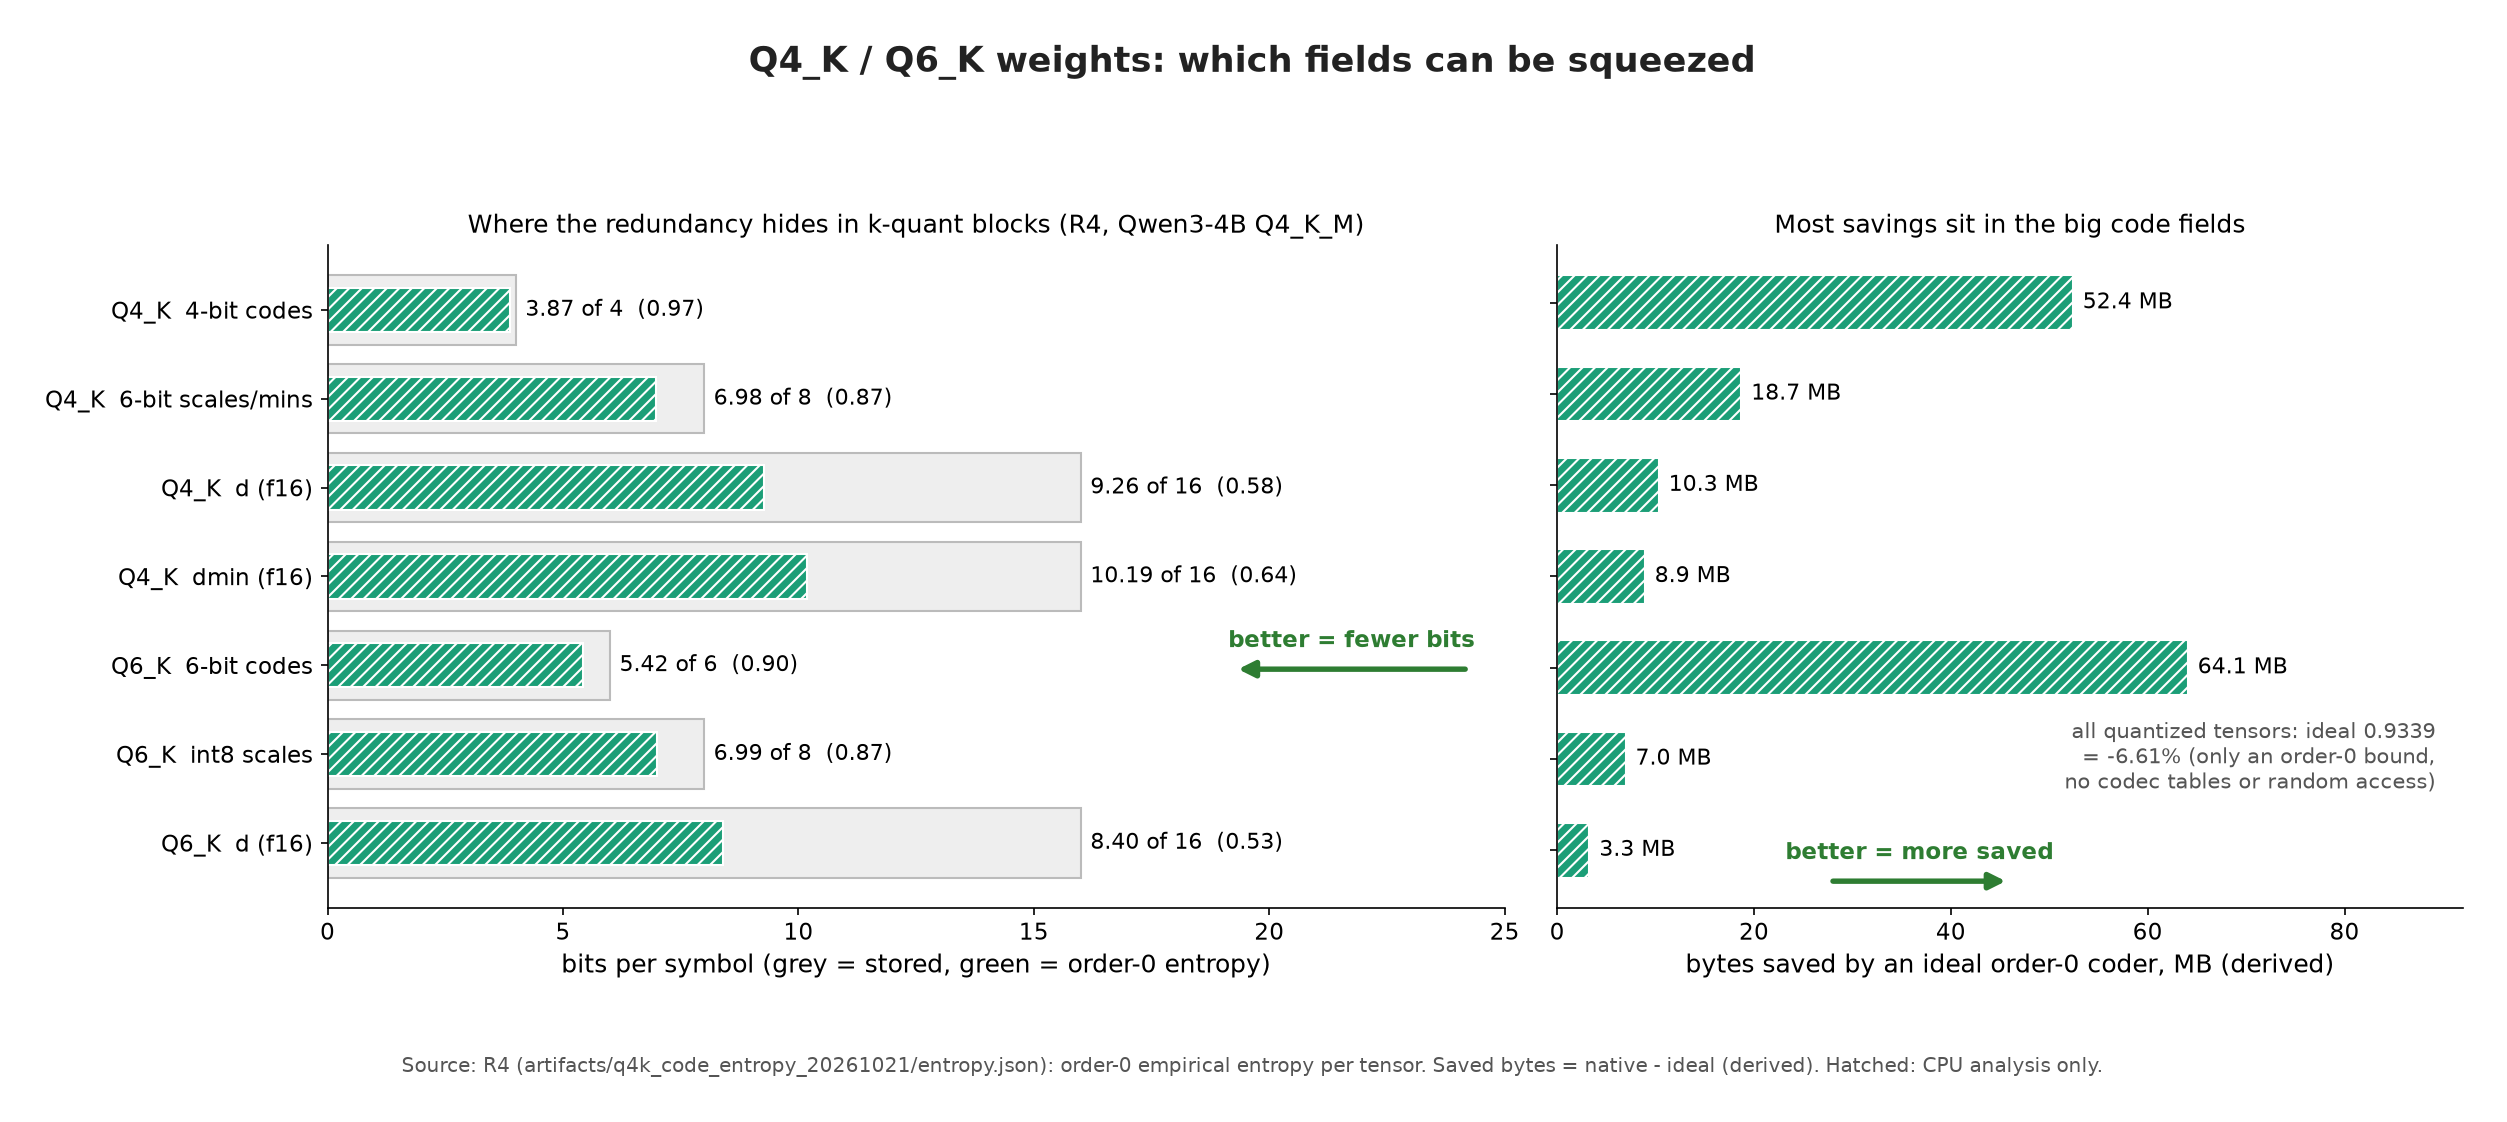
\includegraphics[width=\linewidth]{figures/fig36_k_quant_field_entropy.png}\caption{Which fields of Q4\_K and Q6\_K blocks hold redundancy (R4).}\end{figure}

\begin{figure}[htbp]\centering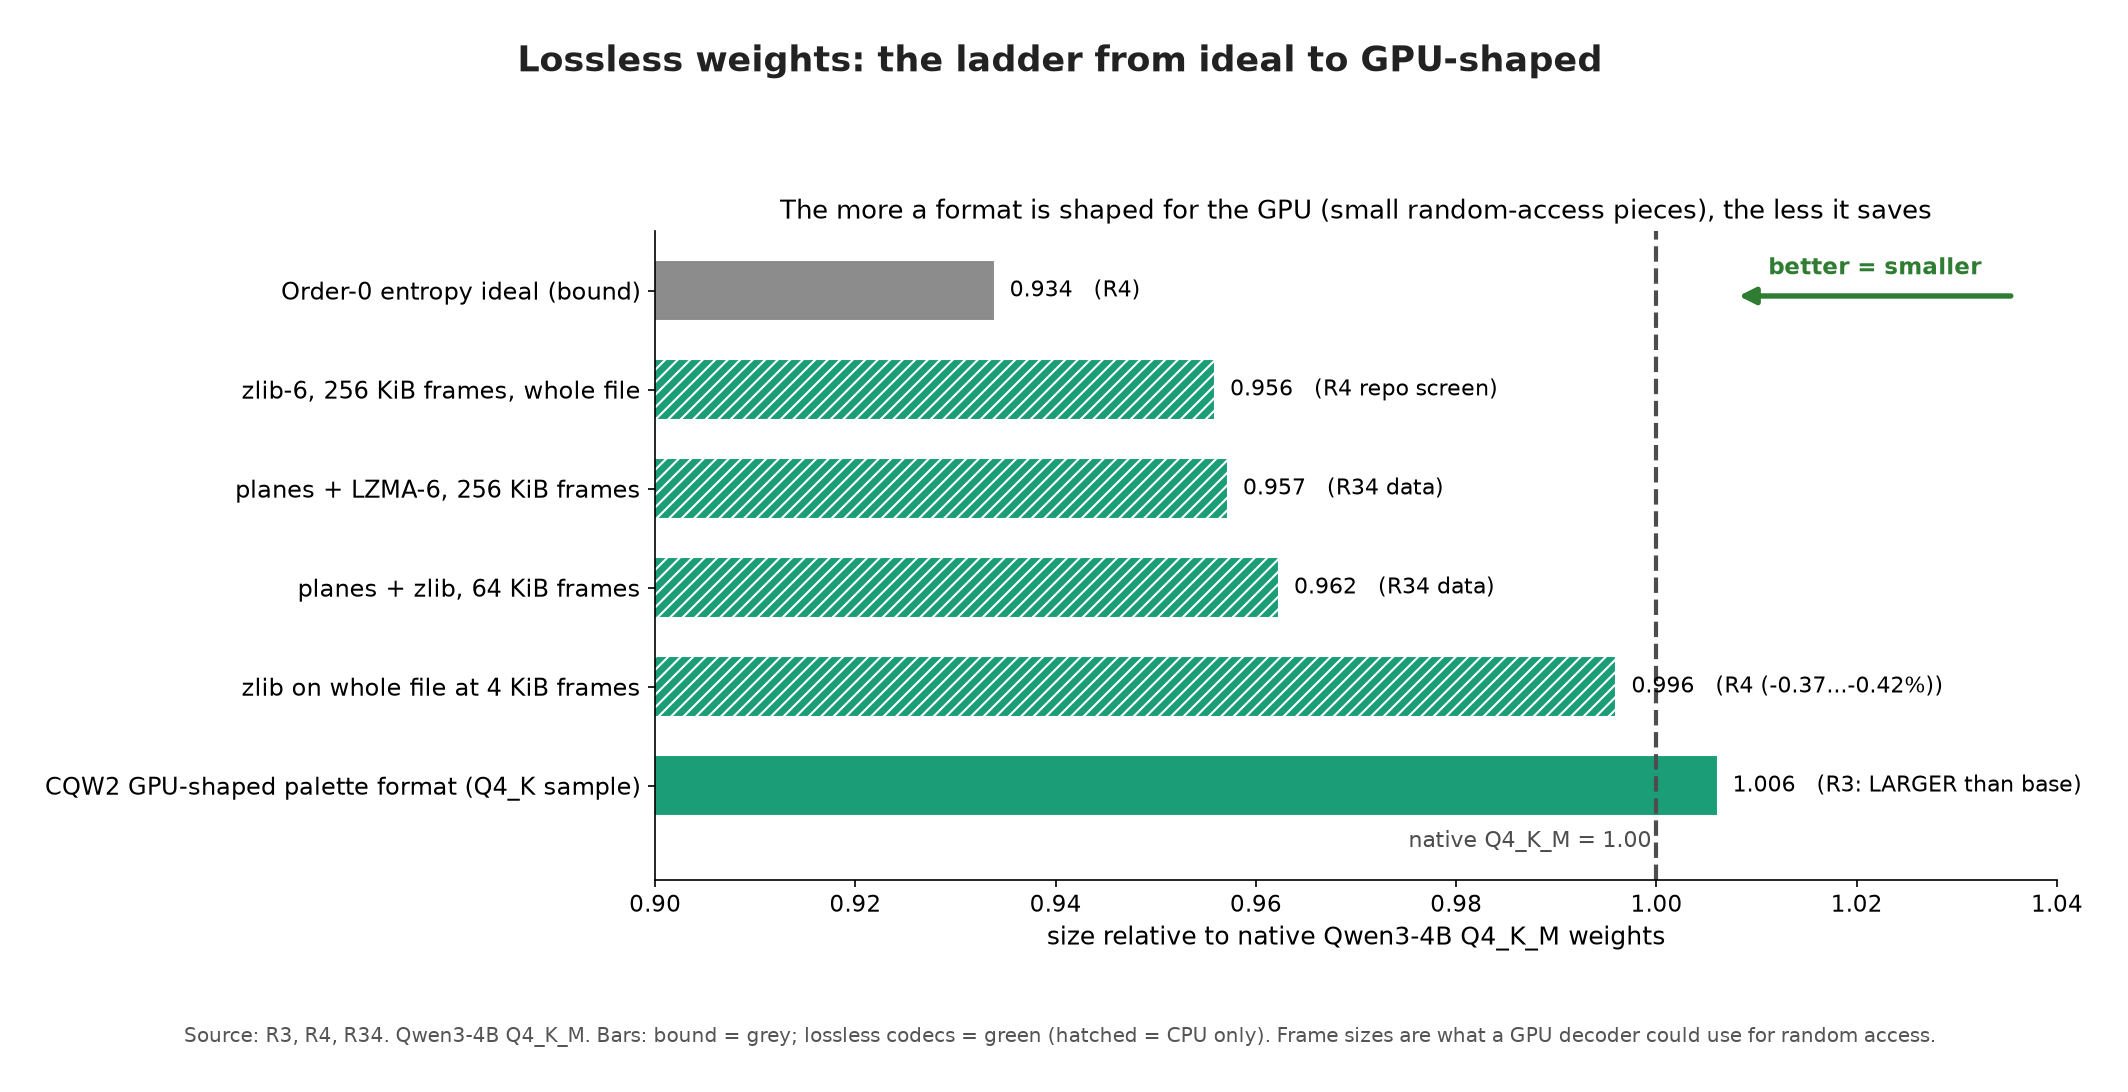
\includegraphics[width=\linewidth]{figures/fig37_weights_headroom_vs_reality.png}\caption{Lossless Q4\_K\_M weights: from the order-0 ideal (0.934) to GPU-shaped formats (CQW2 1.006, larger than the base) (R3, R4, R34).}\end{figure}

\begin{figure}[htbp]\centering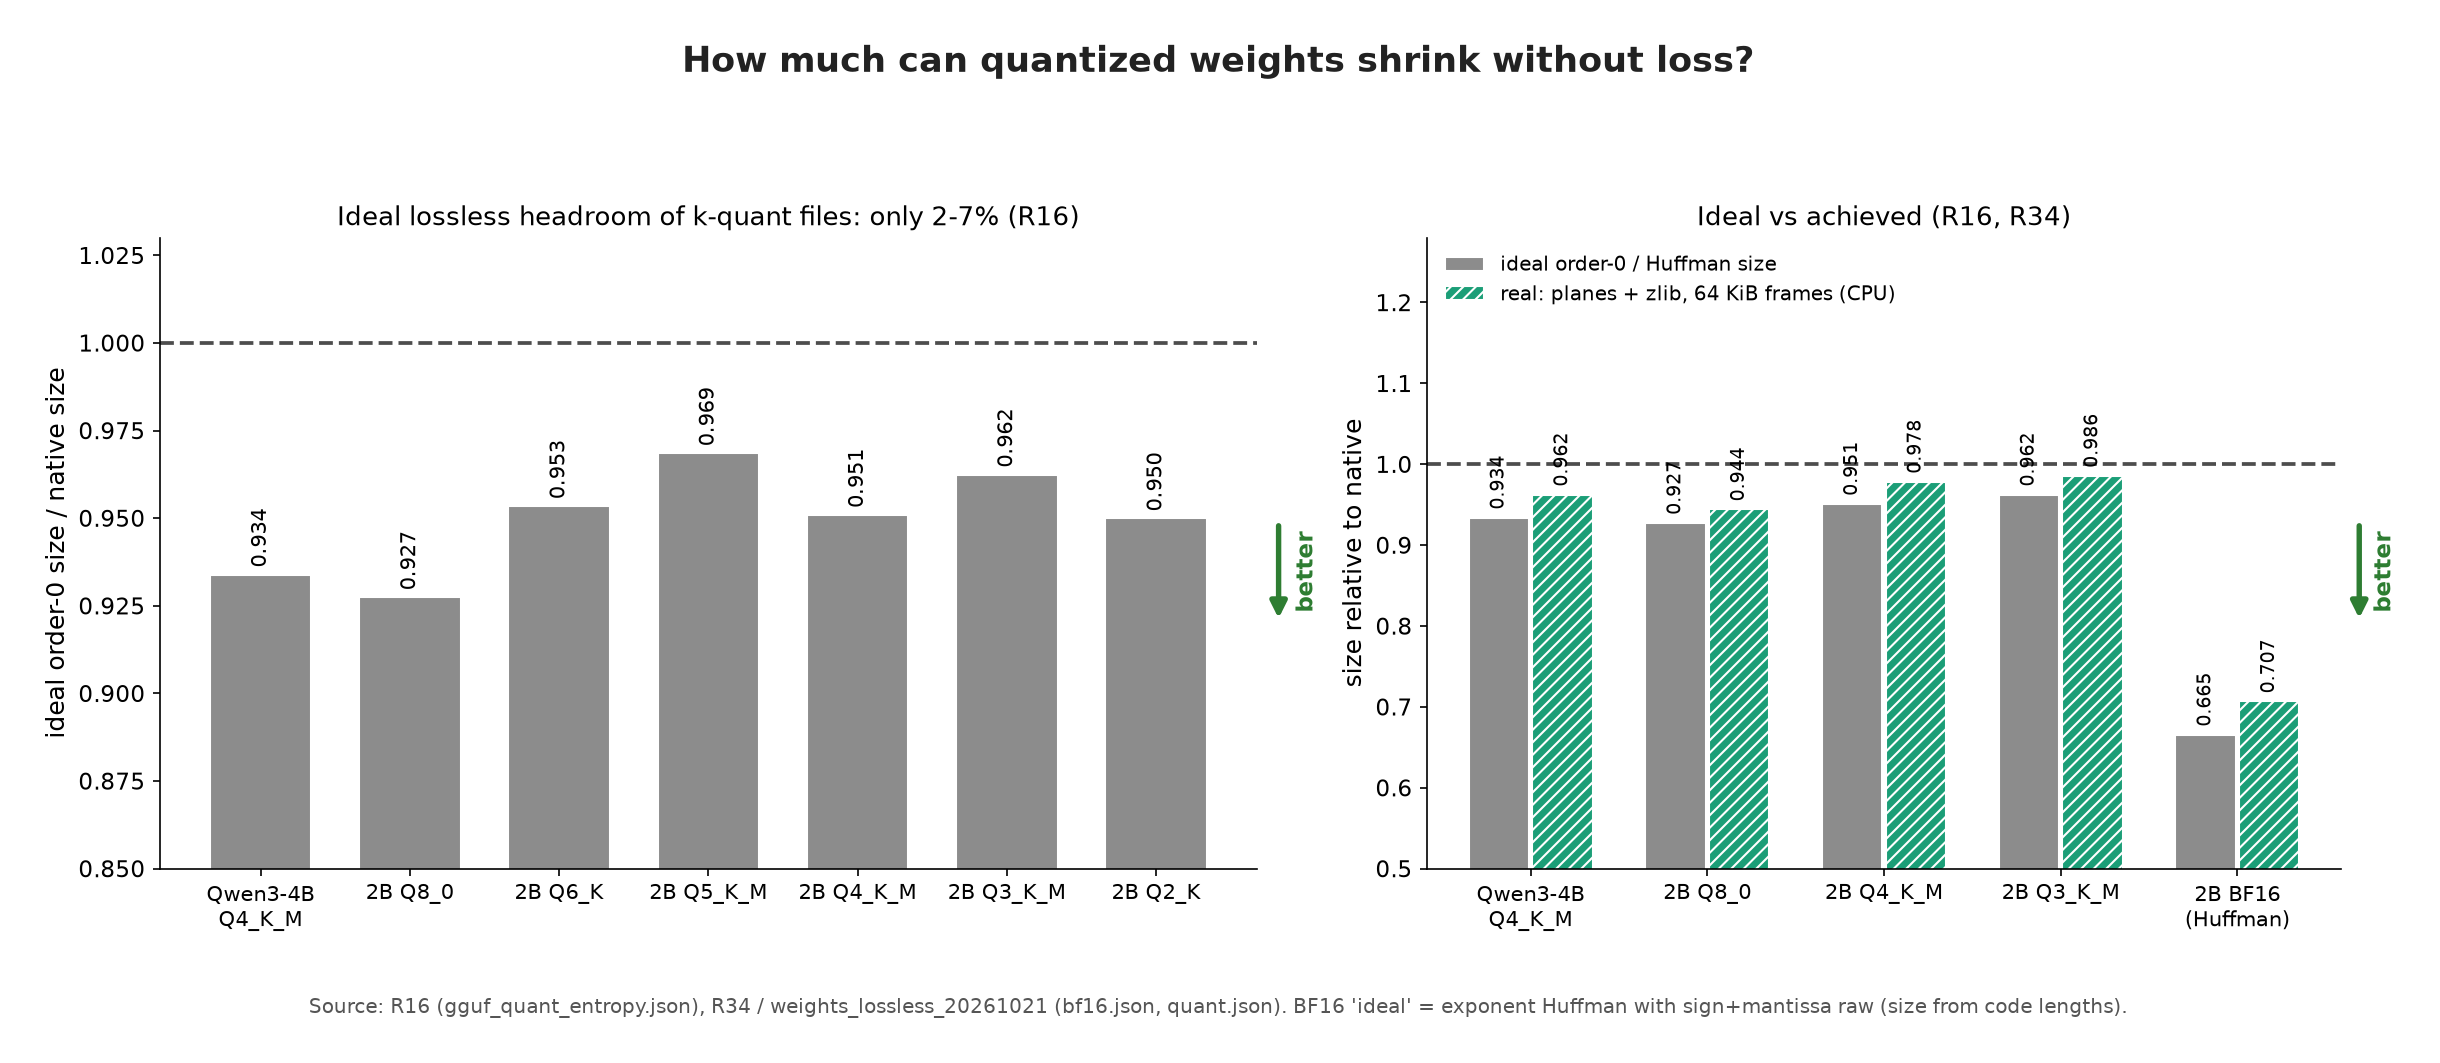
\includegraphics[width=\linewidth]{figures/fig38_weights_lossless_headroom_by_file.png}\caption{Ideal lossless headroom of k-quant files (2--7\%) and what CPU codecs reach (R16, R34).}\end{figure}

\begin{figure}[htbp]\centering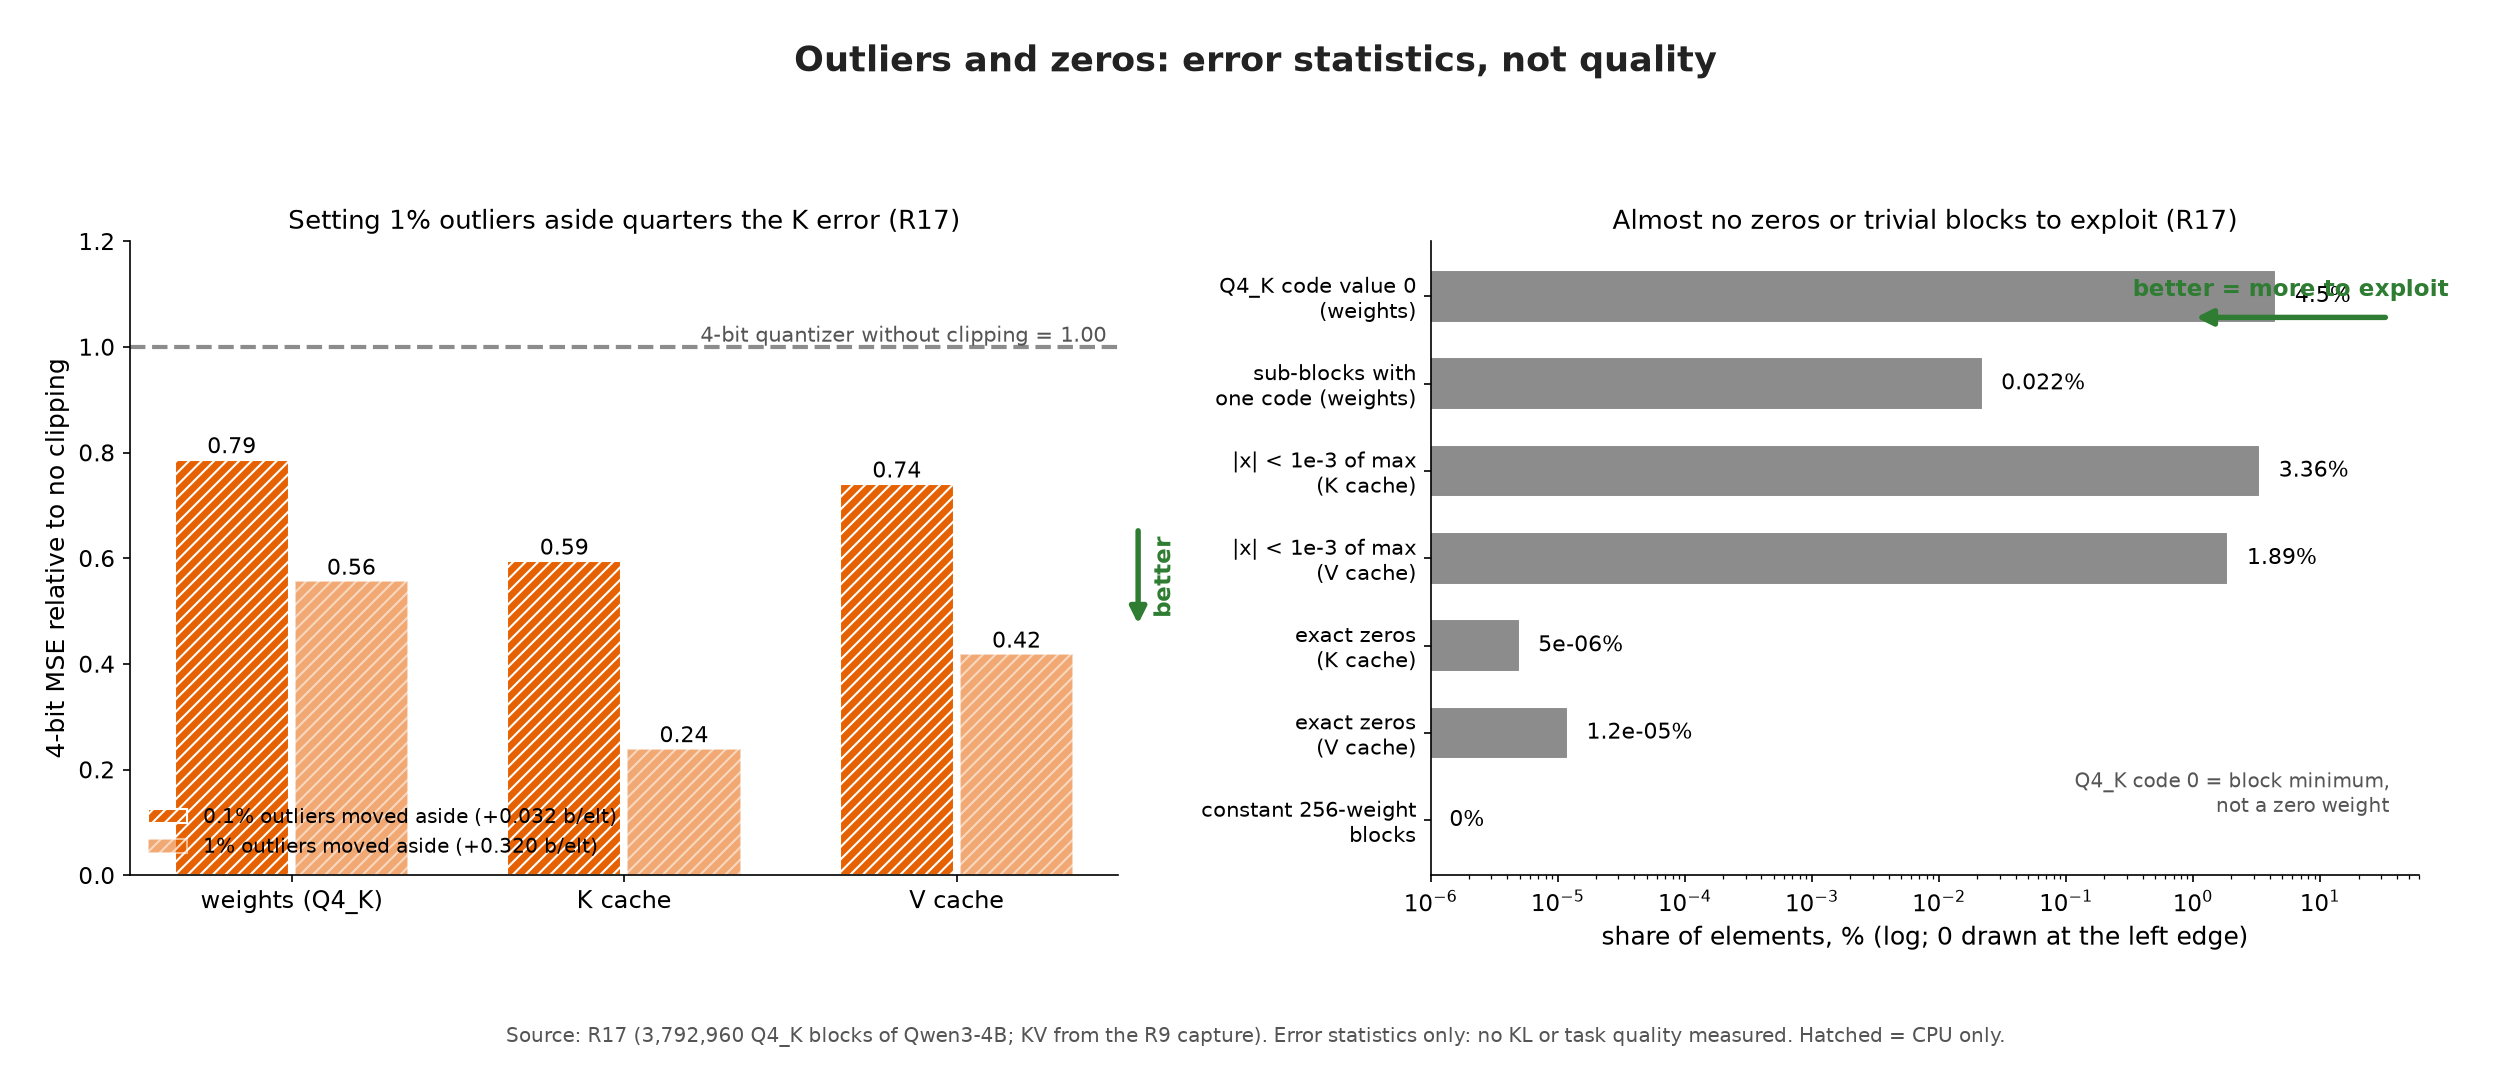
\includegraphics[width=\linewidth]{figures/fig39_outliers_and_sparsity.png}\caption{Outlier clipping and sparsity statistics (R17); error statistics only.}\end{figure}
\end{document}
